


\label{chap:konstruktion}
\chapter{Konstruktion und Design}
\section{Verschiedene Segelbootstypen}
Segelboote weisen eine jahrtausendealte Entwicklungsgeschichte auf. Sie kommen daher in einer unüberschaubahren Zahl von unterschiedlichen Ausgestaltungen vor, die vom einfachen, mit einem Segel versehenen Floss aus Schilf, über mehrmastige Caravellen aus Holz, Freizeitjachten aus Holz, Aluminium oder Kunststoff  bis zur Hightech Rennjacht aus Carbonfasern reicht. Trotz dieser Diversität lassen sich alle Segelboote anhand von drei Hauptmerkmalen (i) Rumpfzahl, (ii) Segelart und (iii) Kielart kategorisieren.\\
\subsection{Rumpfzahl}
Die erste und einfachste Unterscheidung der verschiedenen Segelboottypen erfolgt anhand der Zahl der Rümpfe. Wenn man sich ein Segelboot vorstellt, denkt man meist an ein "mono hull". Jedoch gibt es auch den "double hull" oder man Kategorisiert sie als "multi hull" welche vor allem aus der Welt der Katamarane und Trimarane bekannt sind.\\
Unabhängig von der Unterscheidung nach der Zahl der Rümpfe, lassen sich diese auch nach der Form und dem verwendeten Hauptmaterial unterscheiden.
\subsection{Segelart}
Segel lassen sich grob in flexible und feste Segel einteilen. Flexible Segel bestanden ursprünglich aus Segeltüchern, die aus  Wolle hergestellt wurden. Heute werden für Segeltücher fast ausschiesslich verschiedenene Kunstfasern wie Nylon, Polyester, Kevlar aber auch Carbon verwendet, die zuweilen laminiert werden. 
Festsegel sind steif und fristen ein Nischendahsein. Sie finden sich bisher nur bei expterimentellen Booten und Schiffen aus zwei sehr unterschiedlichen Bereichen. Einerseits können damit grosse Kreuzfahrt- oder Containerschiffe ausgerüstet werden, um deren Energie- und Umwelteffizienz zu verbessern. Dabei kann durch die Verwendung von zusammengesetzten Komposit-Paneelen die mit dem Einsatz textiler Standardsegel verbundene Größenbeschränkung vermieden werde [https://anbord.de/bv-grundsatz-zulassung-fuer-innovatives-festsegel-zusatzantriebssystem-fuer-grosse-kreuzfahrtschiffe/]. Andererseits werden Prototypen für autonome Segelboote und Segelbootdrohnen regelmässig mit Festsegeln ausgerüstet. Diese Boote weisen Längen von 2 bis 20 m auf und die technischen Grössenbeschränkungen textiler Segel sind bei ihnen ohne Relevanz. Sie bestehen bei kommerziellen Projekten aus Verbundwerkstoffen und bei nicht-kommerziellen Projekten meistens aus expandiertem Polystyrol (EPS), das unter dem geschützten Handelsnamen "Styropor" gekannt ist. Der in Form gebrachte Segelkörper wird zum Schutz meistens mit glasfaserverstärktem Kunststoff (GFK) (umgangssprachlich als Fiberglass bezeichnet ) oder anderen Kunststoffen ummantelt.  
\subsection{Kielart}
Segelboote lassen sich in Kiel und Schwertboote unterscheiden. Der Kiel ist der unterste Teil eines Bootsrumpfes. Ein grosser Teil der Segelboote, insbesondere die grössen Boote, verfügt über einen Balastkiel. Ballastkiele sind schwere, aus Gusseisen oder Blei bestehende Kielflossen, die bei Segelbooten für Gewichtsstabilität sorgen. Sie machen etwa ein Drittel bis die Hälfte des gesamten Bootsgewichts aus.
Der Kiel dient beim Segelboot den folgenden zwei Zwecken

(i) Er vergrössert den Lateralplans und vermindert dadurch die seitliche Abdrift des Segelbootes und erzeugt Auftrieb Richtung Luv  (die dem Wind zugewandte Seite). Der Lateralplan ist die seitliche Projektion der Unterwasserfläche des Segelbootes. Er wirkt dem seitlichen Abdriften entgegen. Je größer der Lateralplan ist, desto geringer ist die Abdrift des Wasserfahrzeuges.[https://de.wikipedia.org/wiki/Lateralplan]. Als Abdrift wird das seitliche Versetzen (Abtreiben) von Booten bezeichnet, also die Abweichung vom angestrebten Kurs. Sie umfasst den Einfluss des Windes und der  Strömung.  [https://de.wikipedia.org/wiki/Abdrift]
Ein grosser Lateralplan erlaubt es ein Segelboot hoch am Wind zu segeln (schräg entgegen den Wind voranzukommen). [https://de.wikipedia.org/wiki/Lateralplan]

(ii) Er sorgt für Gewichtsstabilität, die das Segelboot vor dem Kentern (Umkippen) bei starker Krängung (Schräglage) schützt. Der Ballastkiel wirkt als Gegengewicht der Krängung entgegen. Seine Masse  bewirkt  ein aufrichtendes Moment. [https://de.wikipedia.org/wiki/Stabilität_(Schiffskörper)#Gewichtsstabilität]


https://de.wikipedia.org/wiki/Kiel_(Schiffbau)#Ballastkiel

Keinen Kiel haben Flachbodeschiffe wie Jollen oder bestimmte Kuttertypen, die in Flachgewässern operieren. Auch die Mehrrumpfboote verfügen über keinen Kiel. Zur Vermeidung der Abdrift verfügen diese Segelboote an Stelle eins Kiels über ein Schwert, welches beweglich ausgestaltet ist, also eingezogen oder eingeklappt werden kann. Ein Schwert ist ein parallel zur Fahrtrichtung vorgesehene senkrechte Platte aus Stahl, Holz oder glasfaserverstärktem Kunststoff (GFK). 
Ein Schwert vermindert die seitliche Abdrift vor allem durch die größere Fläche im Lateralplan, bei höheren Geschwindigkeiten aber auch durch den dynamischen Auftrieb (der Anteil der auf einen umströmten Körper wirkenden Kraft, der senkrecht zur Anströmrichtung steht [https://de.wikipedia.org/wiki/Dynamischer_Auftrieb]) der anliegenden laminaren Strömung. Mangels Masse schützt ein Schwert, im Gegensatz zu Kielen nicht gegen Kentern. Es dämpft aber durch den seitlichen Wasserwiderstand die Rollbewegungen und stabilisiert so das Boot. [https://de.wikipedia.org/wiki/Schwert_(Schiffbau)]



Der Begriff Stabilität steht im Schiffbau für die Eigenschaft eines Bootes eine aufrechte Schwimmlage einzunehmen und beizubehalten oder sich selbständig wieder aufzurichten, wenn ein krängendes Drehmoment auf das Boot einwirkt oder einwirkte. Krängung ist die Neigung eines Schiffes um seine Längsachse. (https://de.wikipedia.org/wiki/Stabilit%C3%A4t_(Schiffsk%C3%B6rper)).
\begin{figure}
    \centering
    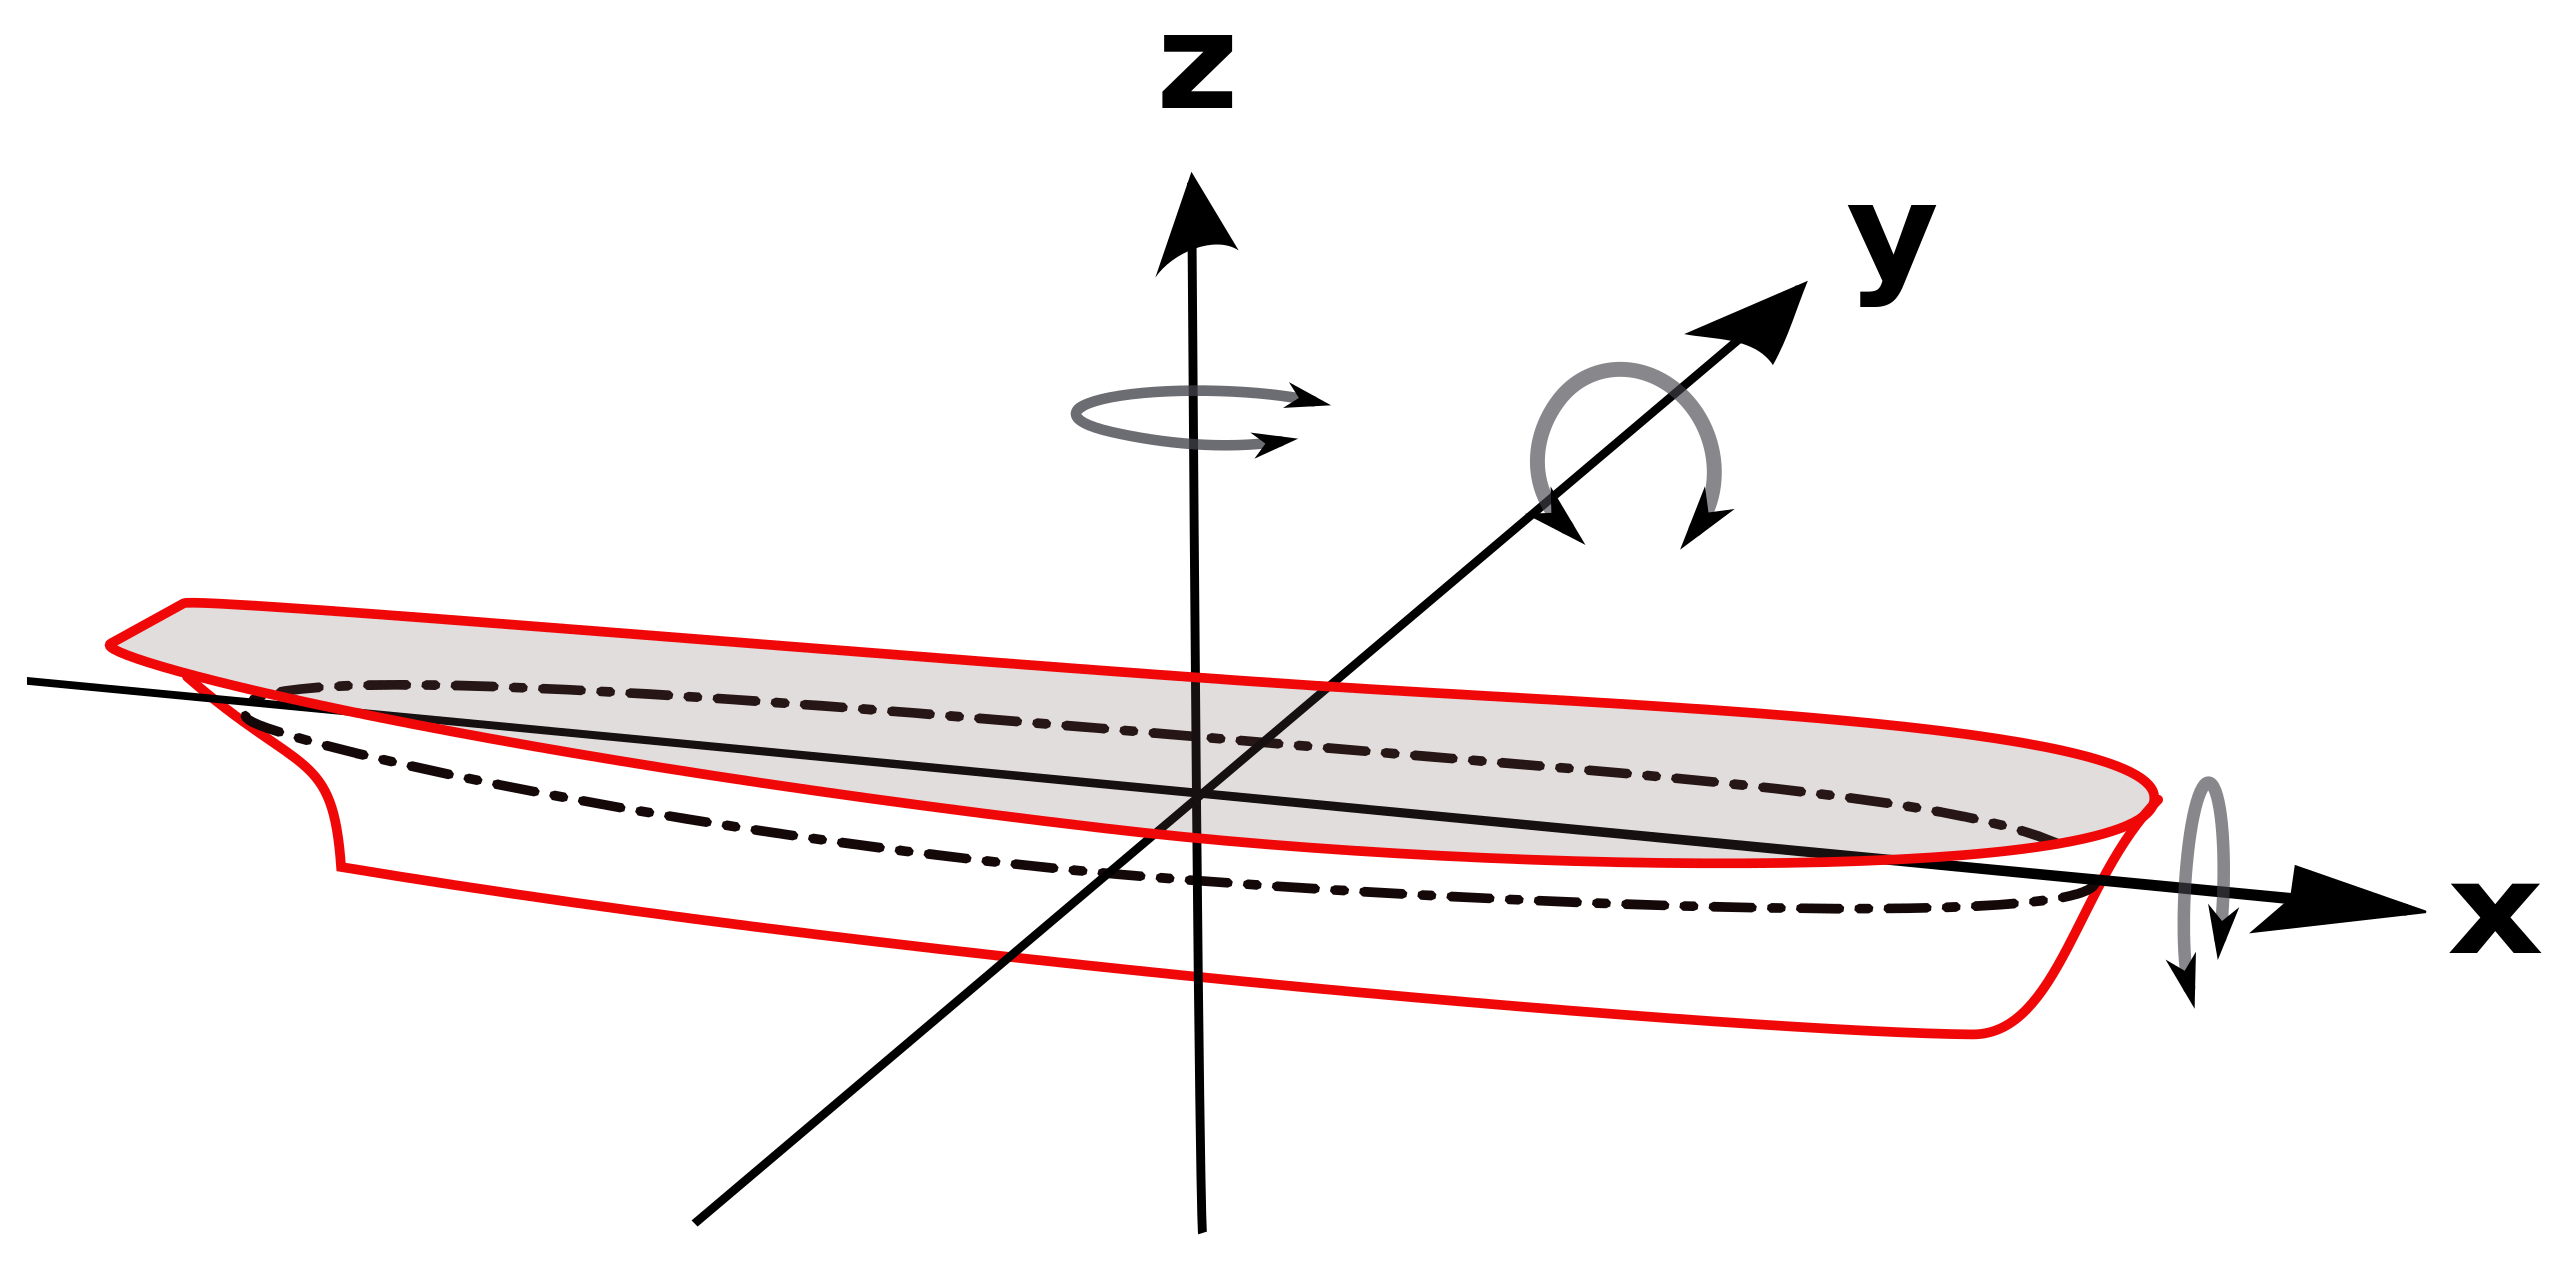
\includegraphics[width=0.5\linewidth]{assets/Achsen_Schiffsbewegung.svg.png}
    \caption{Krängung}
    \label{fig:enter-label}
\end{figure}
Die Stabilität eines Bootes wird durch die drei Parameter Gewichtsschwerpunkt, Auftriebsschwerpunkt (auch Form- oder Verdrängungsschwerpunkt genannt), sowie die sich aus ihnen ergebende sogeannte metazentrische Höhe bestimmt. (https://de.wikipedia.org/wiki/Stabilit%C3%A4t_(Schiffsk%C3%B6rper))  
\\Der Gewichtsschwerpunkt steht für die gesamte in einem Punkt konzentrierte nach unten wirkende Gewichtskraft des Bootes. Seine Lage innerhalb des Bootes  verändert sich bei einer Krängung nicht, solange alle Massen im Boot unverändert an ihrem Ort verharren. \\
Der Auftriebsschwerpunkt steht für die gesamte in einem Punkt konzentrierte nach oben wirkende Gewichtskraft des verdrängten Wassers. Seine Lage ändert sich bei einer Krängung, weil sich durch die Rumpfform auch die „Form“ des verdrängten Wassers ändert.\\
Bei aufrechter Schwimmlage des Schiffes liegt der Gewichtsschwerpunkt exakt vertikal über dem Auftriebsschwerpunkt. Führt ein äusserer Einfluss aber zu einer Krängung des Bootes, verändert sich die Lages des  stehen Gewichtsschwerpunkt auf der horizontalen Achse. Gewichtsschwerpunkt und Auftriebsschwerpunkt stehen  damit nicht mehr senkrecht übereinander. Dadurch entsteht ein aufrichtendes Drehmoment, welches das Boot bei Wegfall des krängenden Einflusses in seine Ausgangslage zurückführt. 
\begin{figure}
    \centering
    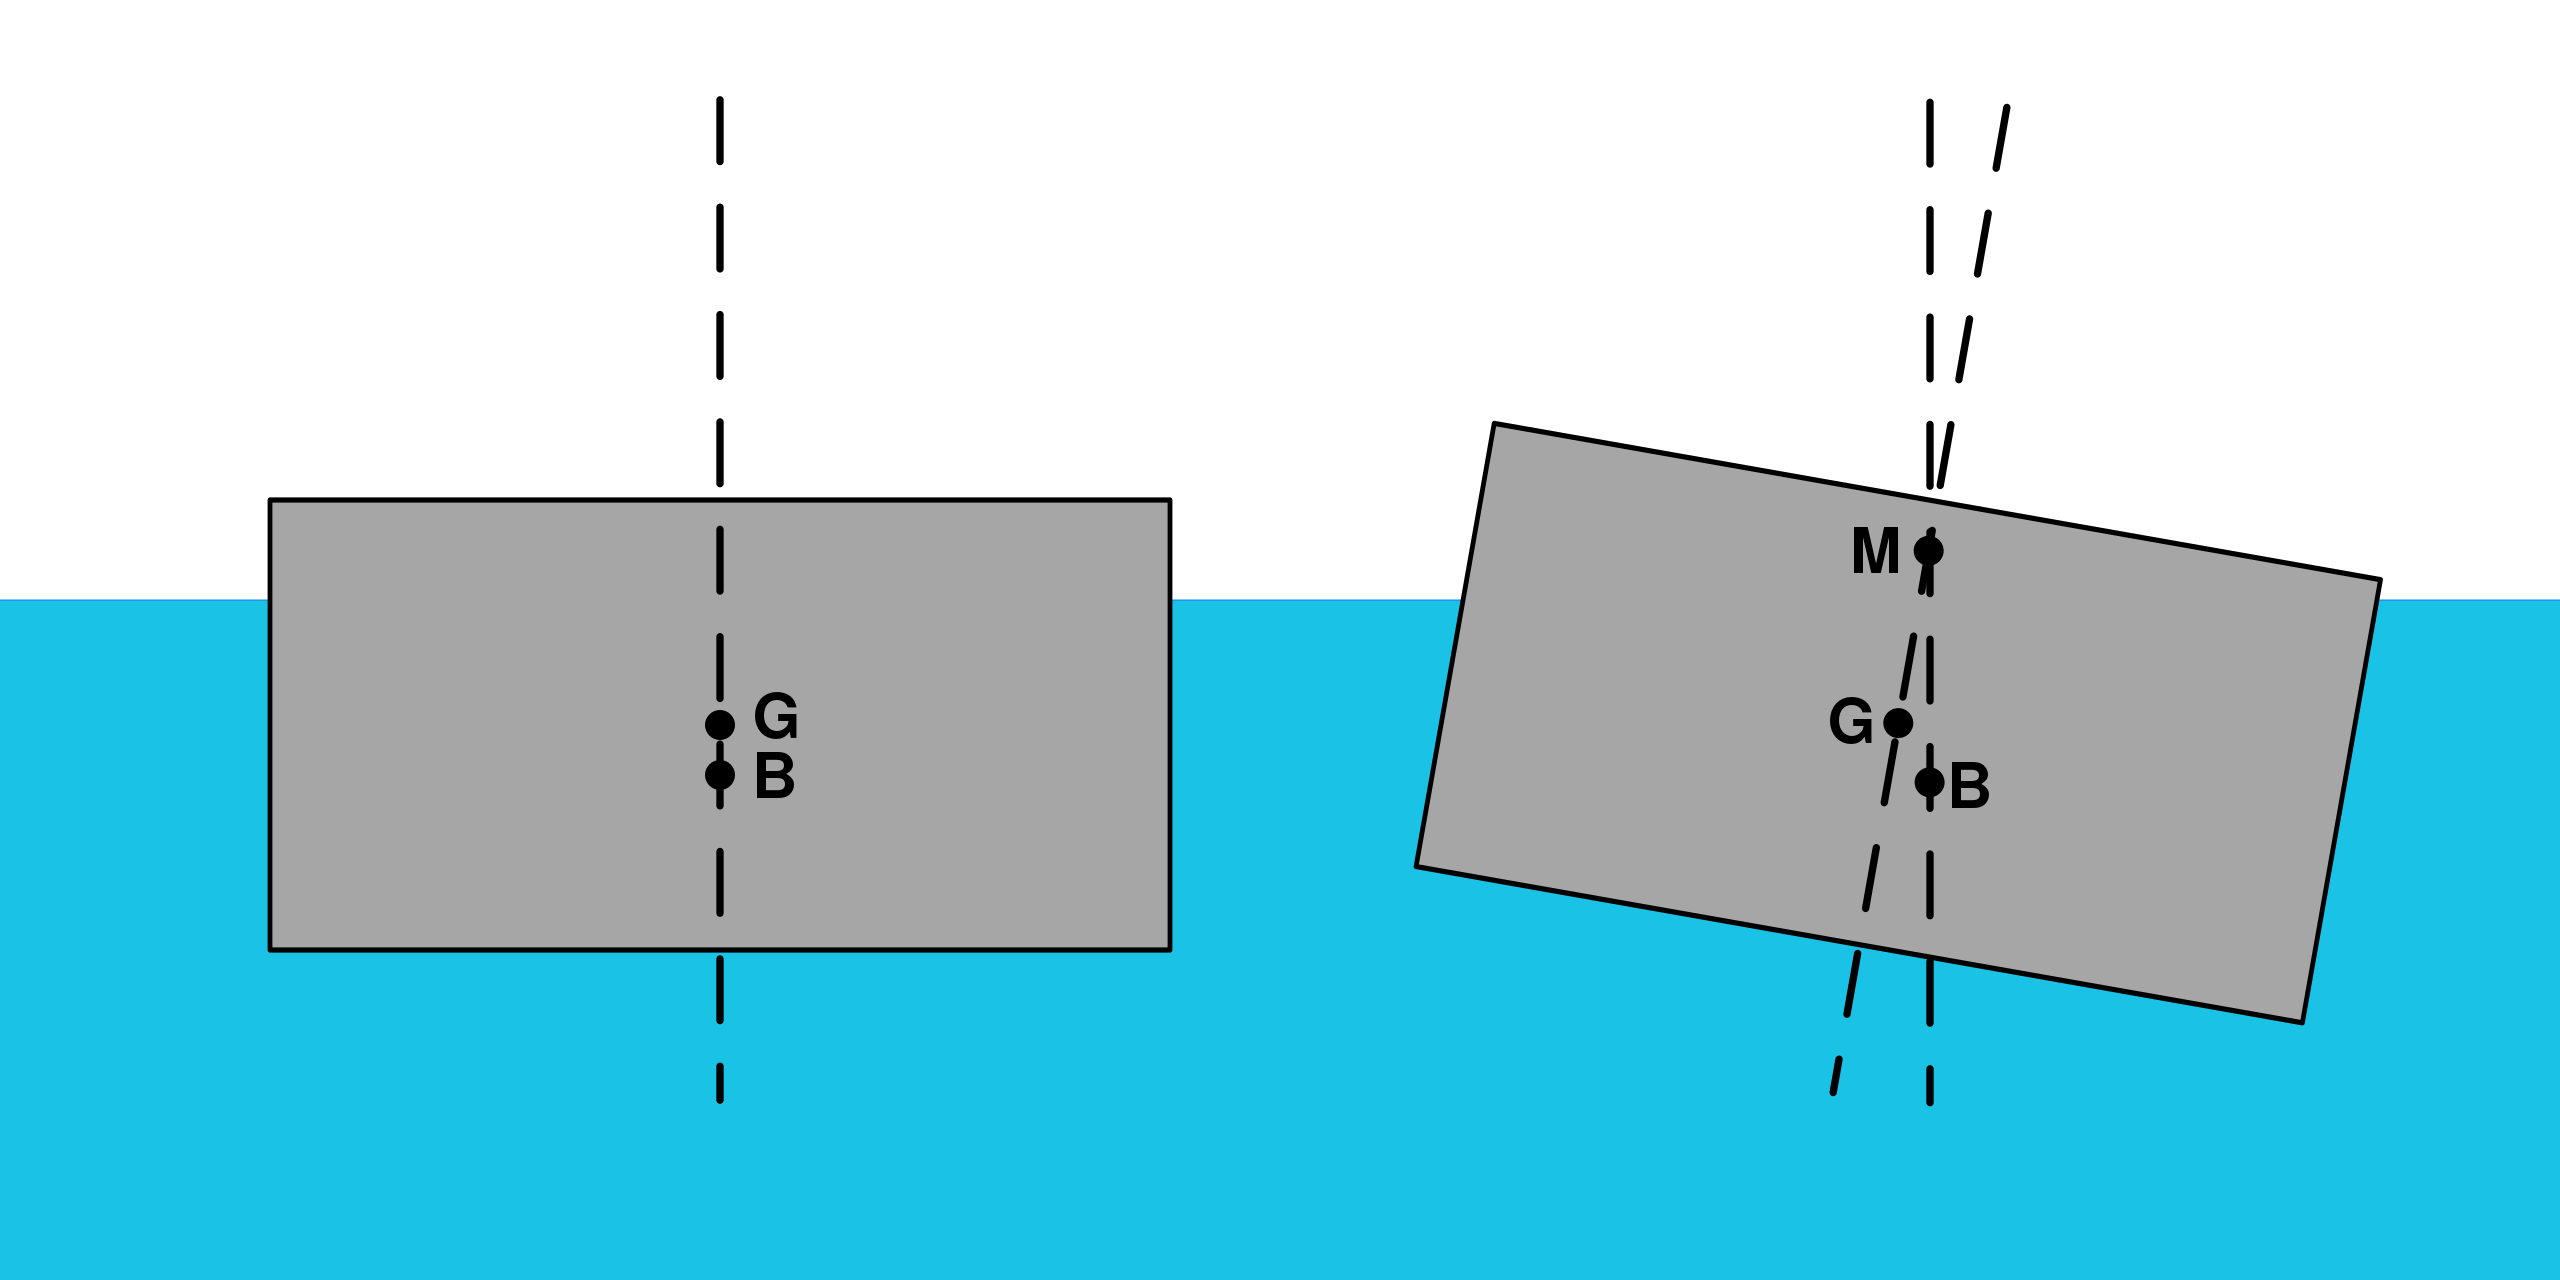
\includegraphics[width=0.5\linewidth]{Metacentriskhojd-svg.svg.png}
    \caption{Lage des Gewichtsschwerpunkt (G), Auftriebsschwerpunkt (B) und Metazentrum (M) bei aufrechtem, sowie gekrängtem Boot }
    \label{fig:enter-label}
\end{figure}
Zur Bewertung der Stabilität eines Schiffes müssen die folgenden drei Parameter bekannt sein: (i) die Anfangsstabilität (die sogeannte metazentrische Anfangshöhe), (ii) der Stabilitätsumfang und (iii) die Fläche unter der Hebelarmkurve. Die metazentrische Höhe ist der Parameter für den aufrichtenden Hebelarm. Mit dem Stabilitätsumfang wird die rechnerische Krängung des Schiffes in Winkelgraden bis zum Kenterpunkt bezeichnet und mit der Hebelarmkurve wird der jeweilige aufrichtende Hebelarm über den vollen Krängungsbereich bis zum Kenterpunkt des Bootes grafisch dargestellt. Der Hebelarm wächst bei zunehmender Krängung zunächst steil an, dann immer flacher an und wird bei noch stärkerer Krängung wieder geringer, bis er schließlich den Kenterpunkt (C) erreicht. Dieser liegt da, wo der Gewichtsschwerpunkt über den Auftriebsschwerpunkt hinauswandert. Mit der Fläche unter der Hebelarmkurve (A) lässt sich die Erfüllung der geplanten Mindeststabilität belegen.  https://de.wikipedia.org/wiki/Stabilit%C3%A4t_(Schiffsk%C3%B6rper))

\begin{figure}
    \centering
    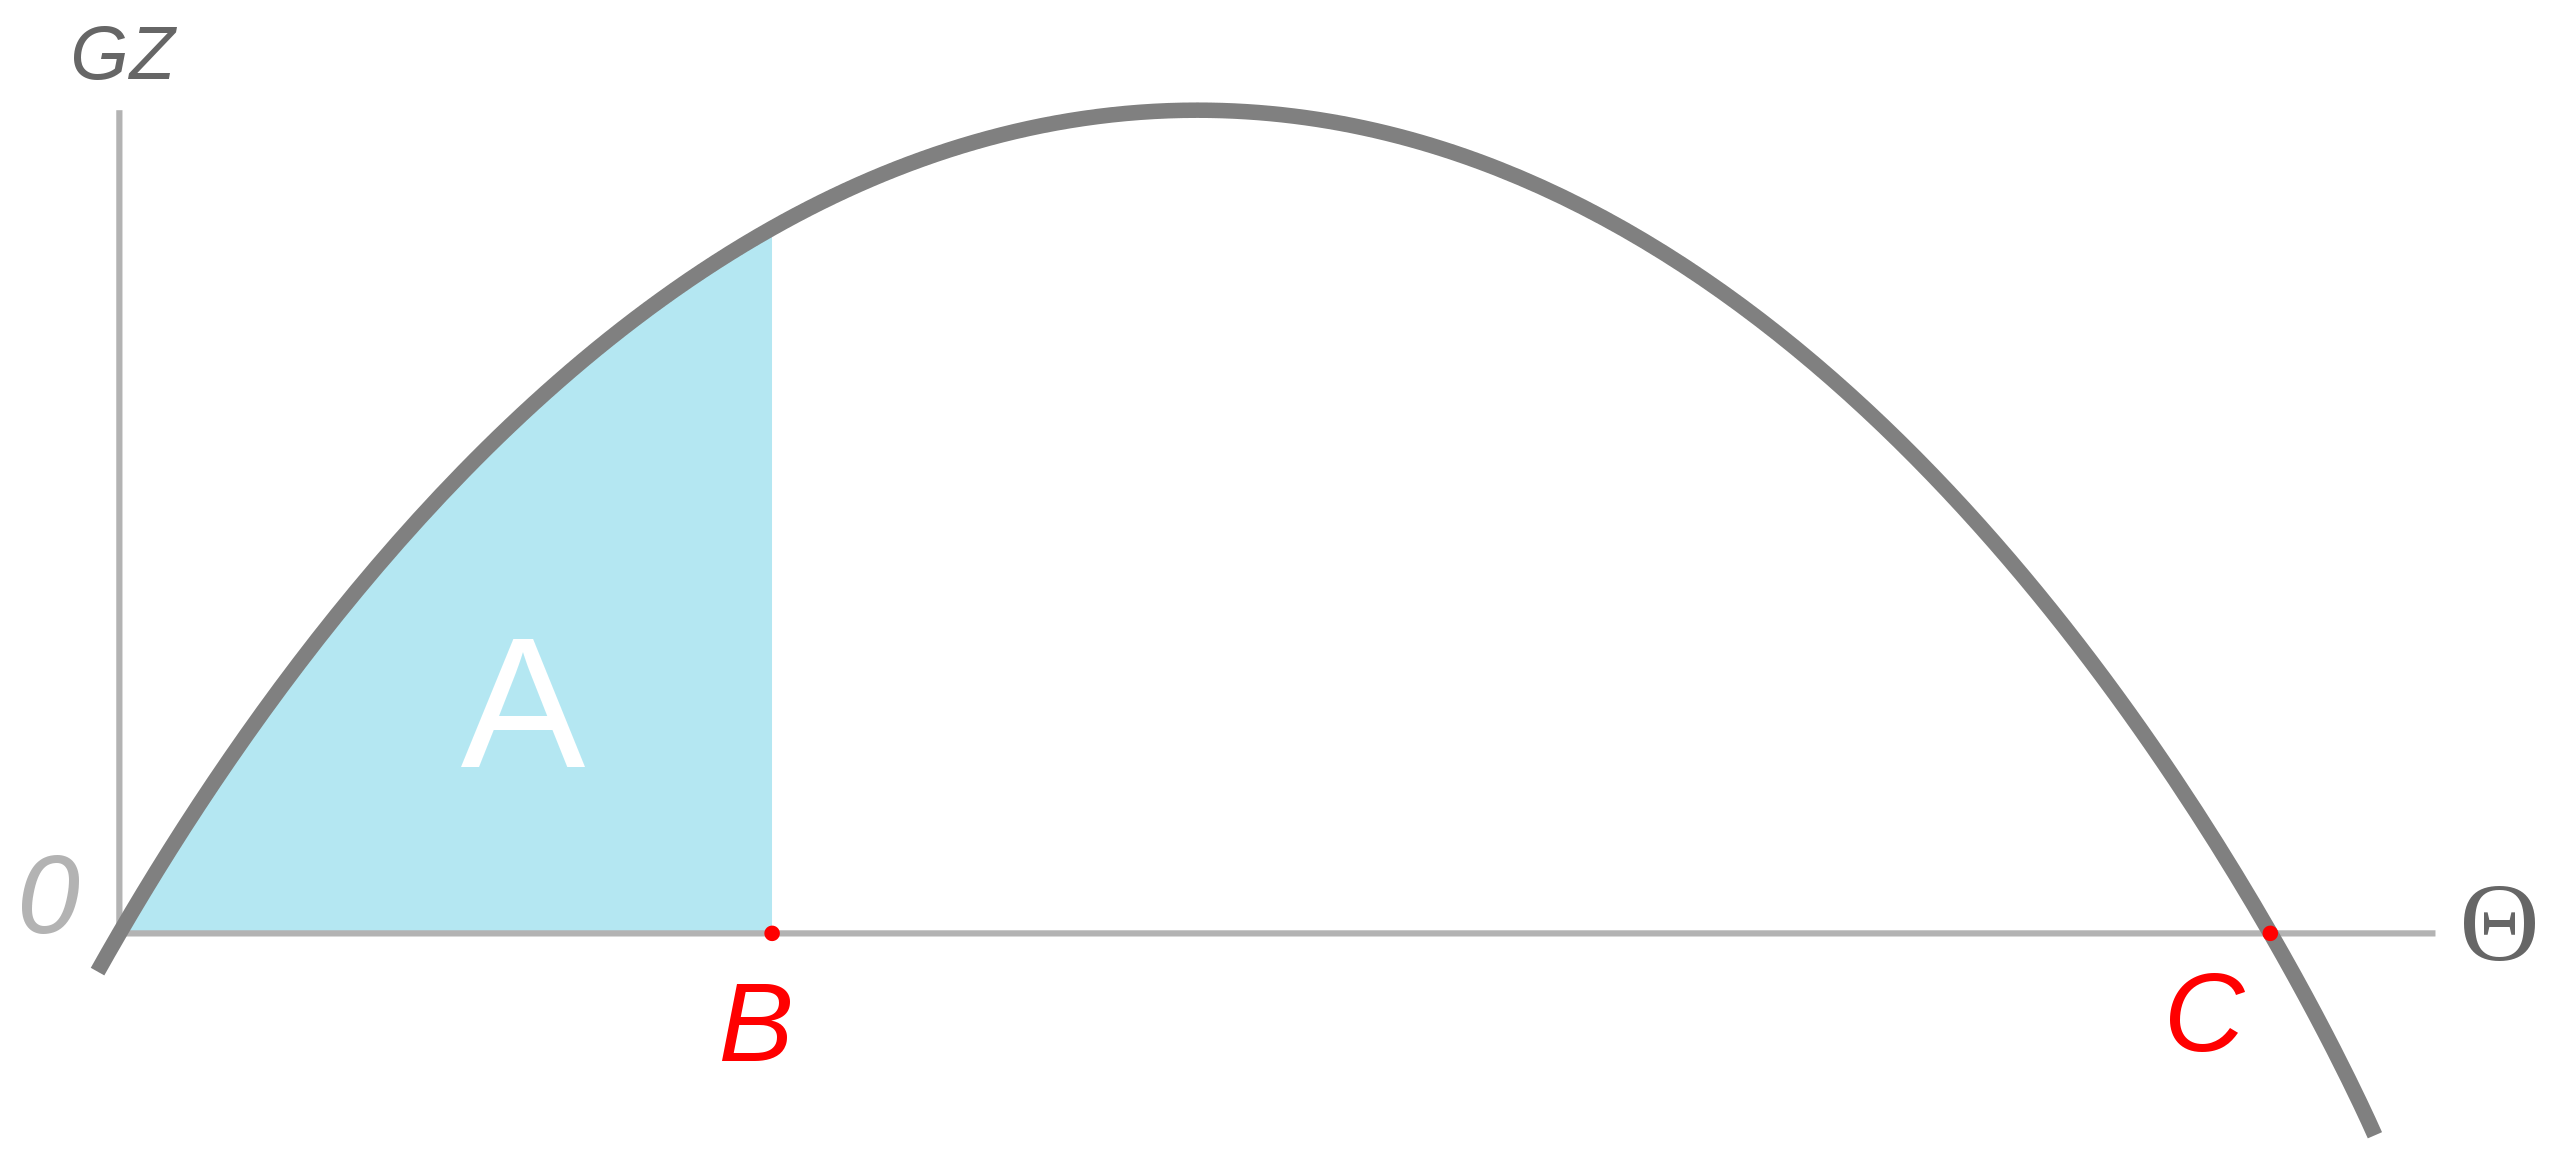
\includegraphics[width=0.5\linewidth]{Stability_curve_NT.svg.png}
    \caption{Hebelarmkurve}
    \label{fig:enter-label}
\end{figure}
Bei Segelbooten sind die Überlegungen zur Stabilität besonders wichtig, da sie mit ihren Segel für den Wind eine sehr grosse Angriffsfläche bieten. Ohne geeignete Gegenmassnahmen kippen sie schon bei geringen Windstärken um. Entscheidnd für die Stabilität eines Segelbootes sind dabei die Rumpfform und Gewichtsverteilung des Bootes. Die Krängung kann durch zwei Massnahmen wieder ausgeglichen und damit die Stabilität erhöht werden: 
\begin{itemize}
    \item Gewichtsstabilität – ein tief liegender Ballastkiel zwingt das Boot wieder in die aufrechte Lage (sogenanntes Stehaufmännchen-Prinzip).
    \item Formstabilität – die Form des Rumpfes begünstigt eine Rückkehr in die Ausgangslage.
\end{itemize}

\paragraph{Gewichtsstabilität}
Gewichtsstabilität durch Ballastkiel
Bei \href{https://de.wikipedia.org/wiki/Segelschiff}{Segelschiffen} wirkt ein \href{https://de.wikipedia.org/wiki/Kiel_(Schiffbau)}{Ballastkiel} als Gegengewicht der \href{https://de.wikipedia.org/wiki/Kr\%C3\%A4ngung}{Krängung} entgegen. Dieser enthält bis zu 50 \% der Masse des Schiffes und bewirkt so ein aufrichtendes Moment. Eine gewisse Krängung unter Segeln – je nach Bauart des Schiffes von 20 bis 45° – ist bei diesen Schiffen normal und stellt keine Gefahr für das Schiff dar. Im untenstehenden Bild ist G der \textit{\href{https://de.wikipedia.org/wiki/Gewichtsschwerpunkt}{Gewichtsschwerpunkt}} (Schwerpunkt des Bootes) und A der \textit{\href{https://de.wikipedia.org/wiki/Formschwerpunkt}{Formschwerpunkt}} (Schwerpunkt der verdrängten Wassermasse). Für mechanische Betrachtungen kann man sich die Gewichtskräfte als im Punkt G vereinigt denken und die Auftriebskräfte als im Punkt A. Mit zunehmender Krängung wandert der Gewichtsschwerpunkt weiter nach außen und es erhöht sich damit das aufrichtende \href{https://de.wikipedia.org/wiki/Drehmoment}{Drehmoment}. Manche Segelschiffe richten sich daher selbst bei einer Krängung von mehr als 120° noch selbstständig wieder auf. Erst durch sehr hohen \href{https://de.wikipedia.org/wiki/Seegang}{Wellengang} können sie mit dem Kiel nach oben gedreht werden und gelten daher als \href{https://de.wikipedia.org/wiki/Kentern}{kentersicher}. Dringen allerdings größere Mengen Wasser ins Bootsinnere, sinken sie wegen des hohen Ballastgewichts. Verliert ein solcher Rumpf, beispielsweise nach einer Grundberührung, seinen Ballastkiel, so ist kaum mehr Stabilität vorhanden und das Kentern faktisch nicht mehr zu verhindern. 
\begin{figure}
    \centering
    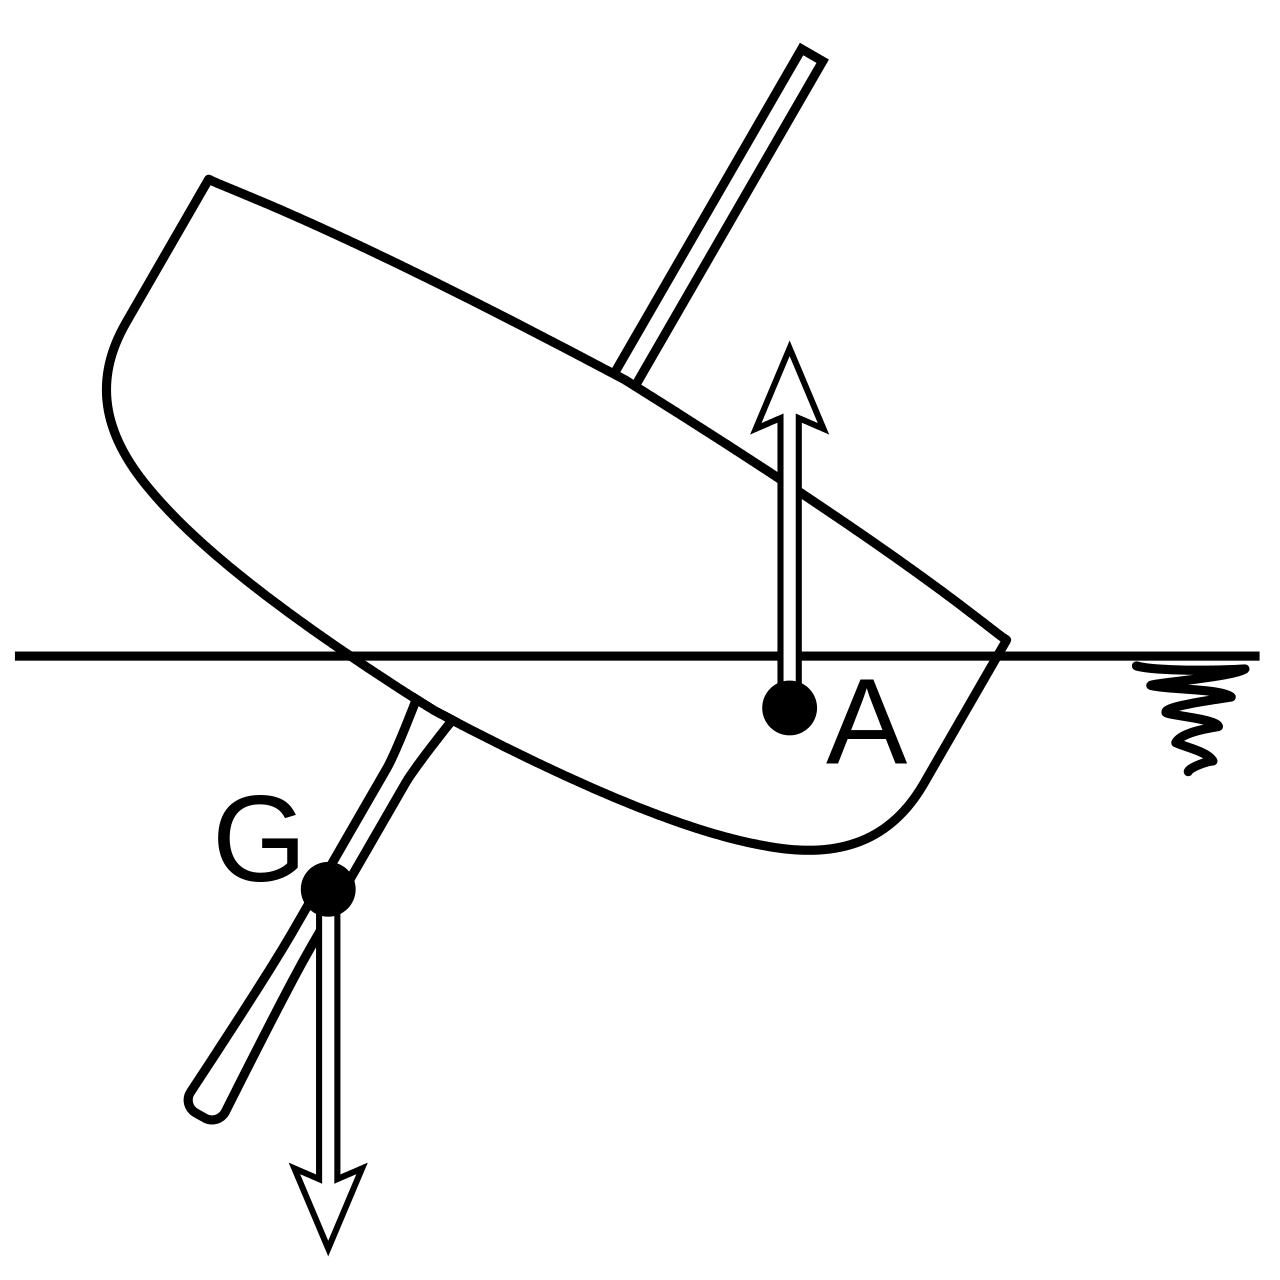
\includegraphics[width=0.5\linewidth]{Segeln_Gewichtsstabilitaet.svg.png}
    \caption{Gewichtsstabilität durch Ballastkiel }
    \label{fig:enter-label}
\end{figure}

\paragraph{Formstabilität}
Im Unterschied zu Kielyachten sind die meisten \href{https://de.wikipedia.org/wiki/Jolle}{Jollen} überwiegend formstabil. Das (meist ausklappbare) leichte Schwert einer Jolle hat keinen nennenswerten aufrichtenden Effekt. Auch \href{https://de.wikipedia.org/wiki/Segelkatamaran}{Katamarane} oder \href{https://de.wikipedia.org/wiki/Trimaran}{Trimarane} haben aufgrund ihrer Breite eine hohe Formstabilität. 
Im untenstehenden Bild ist G der Gewichtsschwerpunkt (Schwerpunkt des Bootes) und A der Formschwerpunkt (Schwerpunkt der verdrängten Wassermasse). In diesen Punkten kann man sich die Gewichts- bzw. Auftriebskräfte vereinigt denken. Für die Formstabilität ist die Lage von A ausschlaggebend. 

Bei aufrechter Lage des Bootes wird auf beiden Seiten des Rumpfes gleich viel Wasser verdrängt. A befindet sich dann mittig im Rumpfquerschnitt, es entsteht kein Drehmoment. Mit zunehmender Krängung (siehe Bild) wird Wasser vor allem auf einer Seite des Rumpfes verdrängt. Dadurch wandert A nach außen, es entsteht ein Drehmoment. Je breiter das Boot ist, desto weiter wandert A nach außen und desto stärker ist das aufrichtende Drehmoment. Wenn die Krängung zu groß wird, nimmt das Drehmoment allerdings wieder ab, weil dann der breite Rumpf gekippt ist und A wieder näher zur Mitte liegt. Eine leichte Krängung wird daher durch das kräftige aufrichtende Drehmoment kompensiert („Wasserwiderstand“), während eine zu starke Krängung zum Kentern des Bootes führt. Katamarane kentern, wenn die Krängung 90° erreicht.\textsuperscript{\href{https://de.wikipedia.org/wiki/Stabilit\%C3\%A4t_(Schiffsk\%C3\%B6rper)\#cite_note-Seemannschaft,_Seite_163-1}{[1]}} 

Es gibt sogar Beispiele für komplett formstabile Bootstypen mit negativer Anfangsstabilität. Diese haben im Ruhezustand keine aufrechte Schwimmlage. 
\begin{figure}
    \centering
    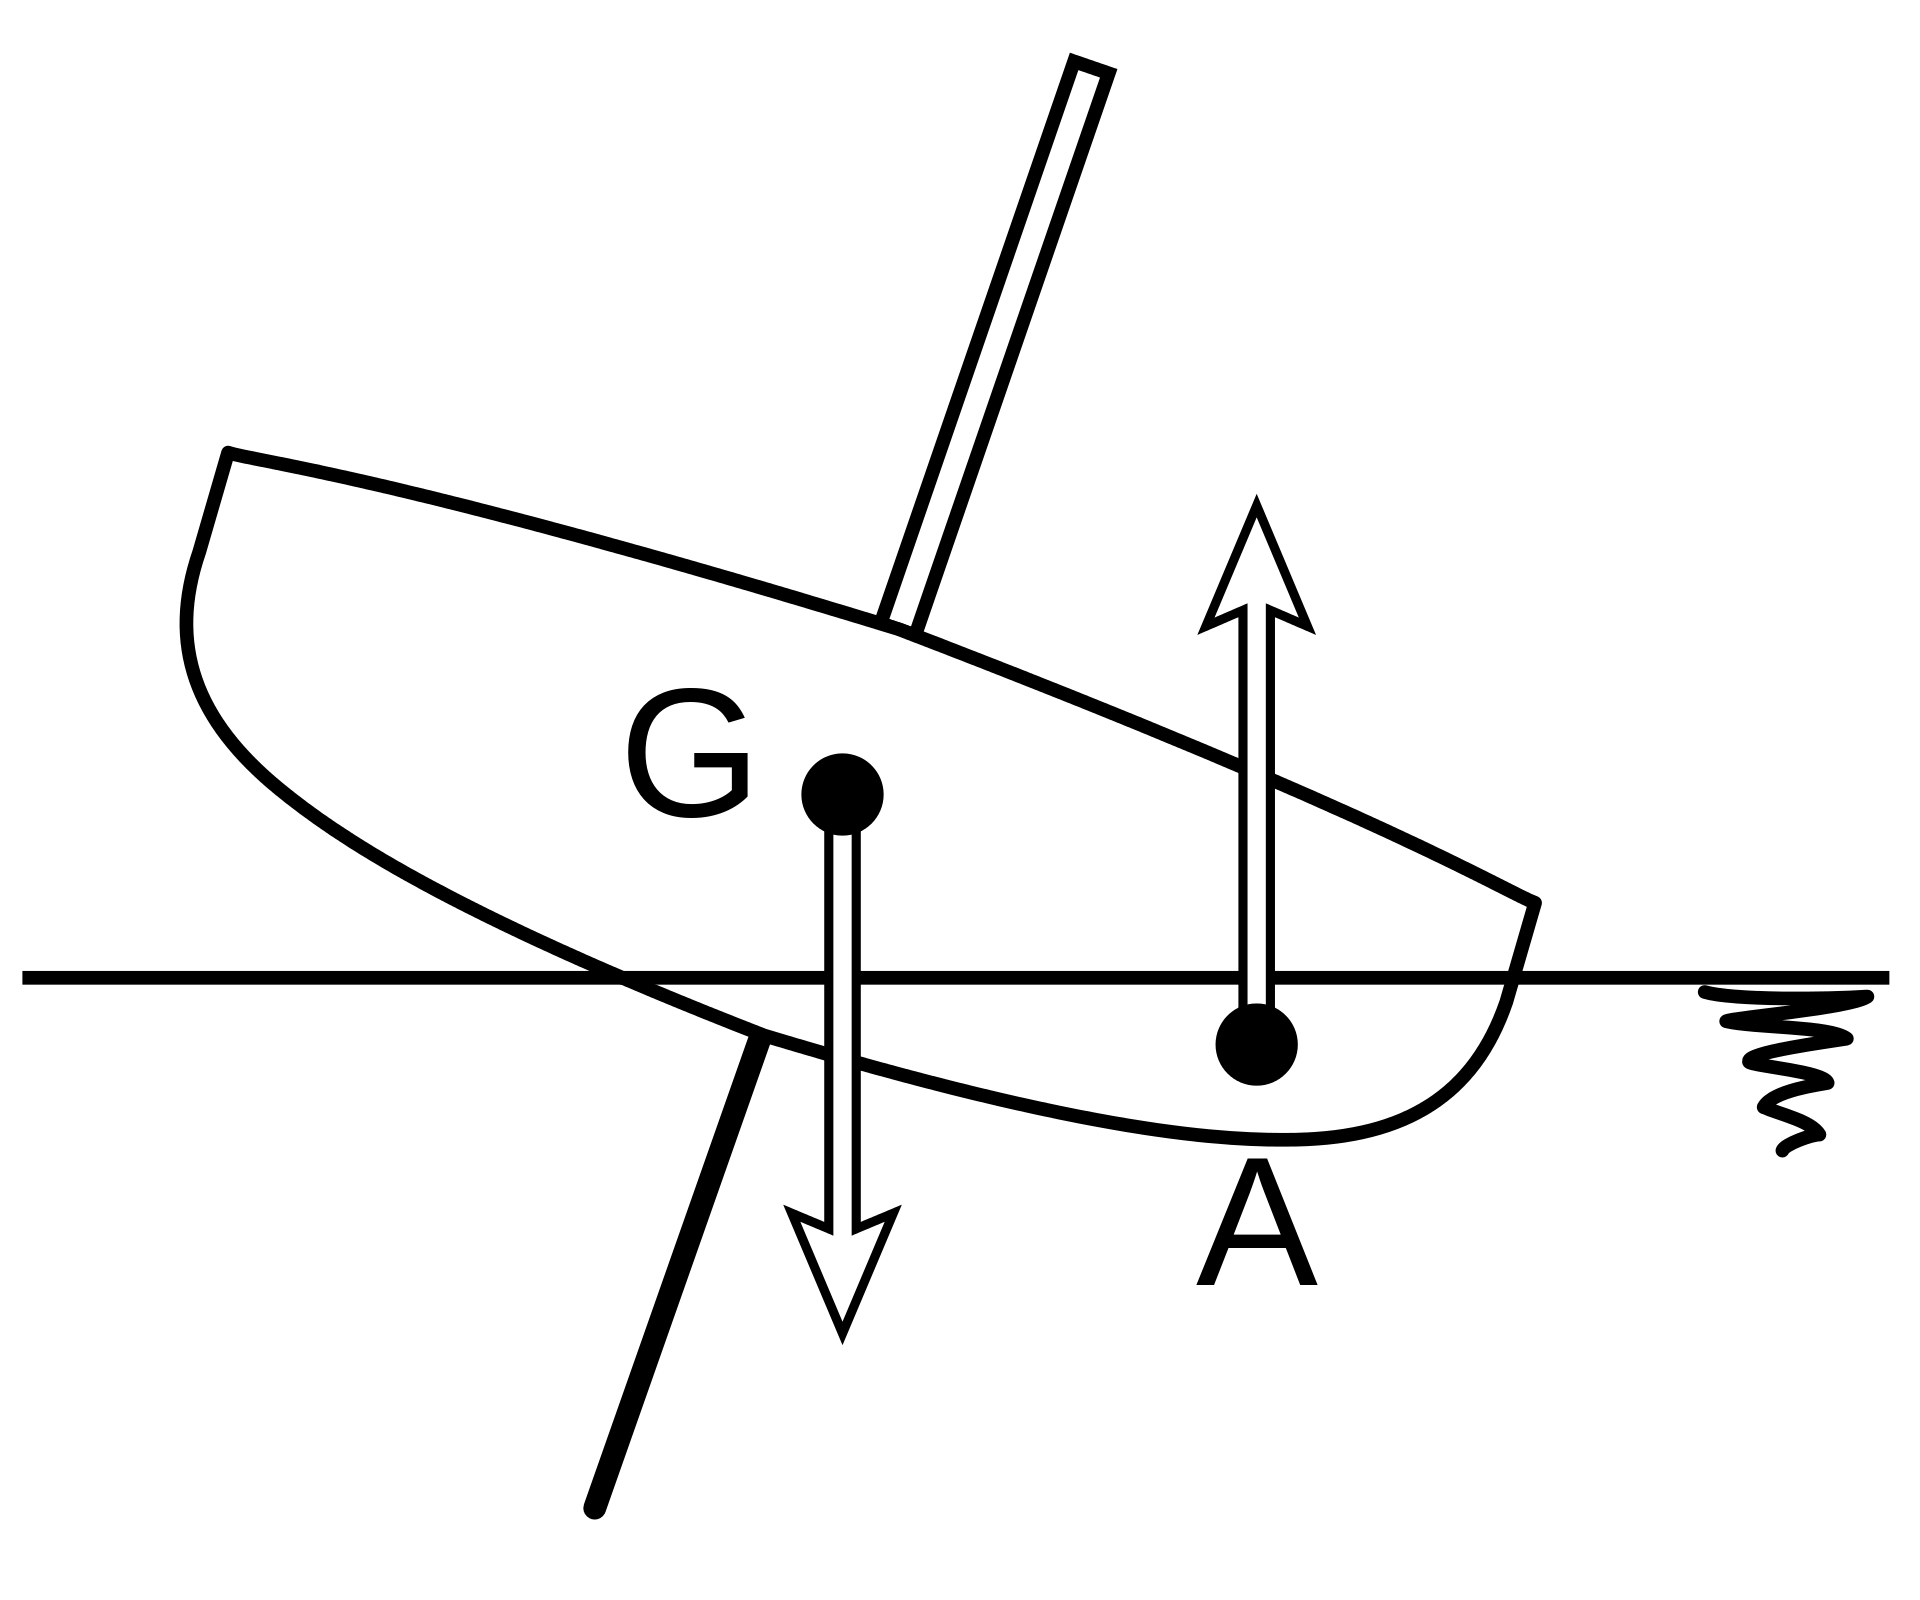
\includegraphics[width=0.5\linewidth]{Segeln_Formstabilitaet.svg.png}
    \caption{Formstabilität }
    \label{fig:enter-label}
\end{figure}

\paragraph{Gegenmaßnahmen bei großer Krängung}

Ein Segler hängt im Trapez, um den Katamaran auszubalancieren.Sowohl bei Kielbooten als auch bei Katamaranen oder Jollen kann die Krängung reduziert werden, indem sich die Crew „auf die hohe Kante setzt“, das heißt sich im \href{https://de.wikipedia.org/wiki/Luv_und_Lee}{Luv} an die Reling setzt, oder die Segelfläche reduziert wird (\href{https://de.wikipedia.org/wiki/Reffen}{Reffen}). Bei sportlich gesegelten \href{https://de.wikipedia.org/wiki/Jolle}{Jollen} hängt sich die Crew in ein \href{https://de.wikipedia.org/wiki/Trapez_(Segeln)}{Trapez}, um weiter nach Luv ausreiten zu können.\textsuperscript{\href{https://de.wikipedia.org/wiki/Stabilit\%C3\%A4t_(Schiffsk\%C3\%B6rper)\#cite_note-2}{[2]}} Beim sportlichen Segeln von Jollen kann eine Kenterung schon mal vorkommen. Sie sind im Gegenzug mit Schwimmkörpern ausgerüstet, so dass sie trotz Kenterung nicht sinken. Jollen sind dennoch nicht für die Hochsee geeignet und selbst gute Jollensegler werden bei angekündigten \href{https://de.wikipedia.org/wiki/Beaufort-Skala}{Windstärken} von mehr als 6 nicht mehr ablegen. 

Durch die Krängung wird automatisch die wirksame Segelfläche reduziert, auch die Form des Rumpfes bevorzugt einen bestimmten Krängungswinkel, bei dem das Schiff die höchste Geschwindigkeit erreichen kann. Daher wird durch starke Krängung das Schiff langsamer, zudem wird der Aufenthalt an Bord ungemütlicher. Auch steigt die Gefahr, dass es durch zu starke Krängung zu einem sogenannten \href{https://de.wikipedia.org/wiki/Sonnenschuss}{Sonnenschuss} kommt und das Schiff „aus dem Ruder läuft“\textsuperscript{\href{https://de.wikipedia.org/wiki/Stabilit\%C3\%A4t_(Schiffsk\%C3\%B6rper)\#cite_note-3}{[3]}} und „in den Wind schießt“.\textsuperscript{\href{https://de.wikipedia.org/wiki/Stabilit\%C3\%A4t_(Schiffsk\%C3\%B6rper)\#cite_note-4}{[4]}} Noch schlimmer ist es, wenn die Nock des \href{https://de.wikipedia.org/wiki/Baum_(Segeln)}{Großbaums} ins Wasser eintaucht, was zu schweren Schäden am \href{https://de.wikipedia.org/wiki/Takelage}{Rigg} führen kann. Daher kann durch rechtzeitiges Reffen – trotz verkleinerter Segelfläche – die Geschwindigkeit zunehmen. 

 Schwertboote haben \href{https://de.wikipedia.org/wiki/Formstabilit\%C3\%A4t}{formstabile} \href{https://de.wikipedia.org/wiki/Schiffsrumpf}{Rümpfe}. Ihr aufrichtendes \href{https://de.wikipedia.org/wiki/Drehmoment}{Drehmoment} wird nicht wie bei \href{https://de.wikipedia.org/wiki/Kielboot}{Kielbooten} durch einen \href{https://de.wikipedia.org/wiki/Kiel_(Schiffbau)\#Flossenkiel}{Ballastkiel}, sondern durch entsprechende Formgebung des Rumpfquerschnittes erreicht. Schwertboote sind im Allgemeinen relativ breit. Die \href{https://de.wikipedia.org/wiki/Schiffsmast}{Masthöhe} und die gefahrene \href{https://de.wikipedia.org/wiki/Segelfl\%C3\%A4che}{Segelfläche} sind im Verhältnis zur Rumpfgröße geringer als bei Kielbooten. Schwertboote besitzen bei leichter \href{https://de.wikipedia.org/wiki/Kr\%C3\%A4ngung}{Krängung} (Neigung) ein sehr hohes aufrichtendes Moment aufgrund ihrer Formstabilität. Dieses aufrichtende Moment nimmt jedoch mit zunehmender Krängung stark ab, so dass es zur \href{https://de.wikipedia.org/wiki/Kenterung}{Kenterung} kommen kann. Bei Kielbooten ist es umgekehrt, bei leichter Krängung ist das aufrichtende Moment gering und nimmt bei zunehmender Krängung zu, sodass sie kaum kentern können bzw. sich nach einer Kenterung von alleine wieder aufrichten.  (https://de.wikipedia.org/wiki/Schwertboot)


 Der Kiel bei Segelbooten}

Bei Segelbooten erfüllt der Kiel zusätzlich zwei weitere Funktionen: 

\begin{enumerate}
    \item Er dient der Vergrößerung des \href{https://de.wikipedia.org/wiki/Lateralplan}{Lateralplans}, der die seitliche \href{https://de.wikipedia.org/wiki/Abdrift}{Abdrift} des Fahrzeugs vermindert und Auftrieb Richtung Luv erzeugt. Dies ermöglicht Segelfahrzeugen, hoch \href{https://de.wikipedia.org/wiki/Kurse_zum_Wind}{am Wind} zu segeln (schräg entgegen den Wind voranzukommen).
    \item Er sorgt für \href{https://de.wikipedia.org/wiki/Stabilit\%C3\%A4t_(Schiffsk\%C3\%B6rper)\#Gewichtsstabilit\%C3\%A4t}{Gewichtsstabilität}, die das Fahrzeug vor dem \href{https://de.wikipedia.org/wiki/Kentern}{Kentern} (Umkippen) bei starker \href{https://de.wikipedia.org/wiki/Kr\%C3\%A4ngung}{Krängung} (Schräglage) schützt.
\end{enumerate}
Für maximale Wirkung und gute Segeleigenschaften sollte das Kielgewicht so tief und so schwer wie möglich sein. Besonders in flachen Binnengewässern führt das allerdings zu erheblichen Einschränkungen bei der Wahl der möglichen Anlegehäfen, weshalb man hier vermehrt auf Hubkiele setzt oder anderweitige Kompromisse eingehen muss. Segelschiffe mit festem Kiel haben einen deutlich größeren \href{https://de.wikipedia.org/wiki/Tiefgang}{Tiefgang} als vergleichbare Motorschiffe. 

Schiffsmodelle aus über 50 Jahren Yachtbau. Gut erkennbar ist die Veränderung des Unterwasserschiffs über die Jahrzehnte (im Bild beispielhaft die diversen Yachten des deutschen Seglers \href{https://de.wikipedia.org/wiki/Hans-Otto_Sch\%C3\%BCmann}{Hans-Otto Schümann})Der hydrodynamische Auftrieb des Unterwasserschiffs wirkt in Richtung Luv und hält so das Schiff auf Kurs (siehe \href{https://de.wikipedia.org/wiki/Physik_des_Segelns}{Physik des Segelns}). Erkenntnisse aus der Strömungslehre ermöglichen es, effiziente Kielformen am Computer zu bestimmen. Die Wirksamkeit des Kiels als Auftriebsflosse ist in erster Näherung lediglich vom Quadrat des Tiefgangs, nicht aber von der Fläche des Unterwasserschiffs abhängig. Deshalb haben sich die Formen der Kiele in den letzten 50 Jahren deutlich verändert. Waren zu Beginn des modernen Yachtbaus noch lange Kiele üblich, sind sie heute sehr schmal und tief. 

 




\section{Wahl des Bootstypus}
\subsection{Wahl der Segelart}
Ausgangspunkt für die Wahl des Bootstypus für das vorliegende Projekt bildet der Entscheid über das zu verwendende Segel. Da sich das Segelboot autonom bewegen können muss, fällt dieser Entscheid leicht. Nur mit einem Festsegel lässt sich die Neigung flexibler Segel zu flattern vermeiden. 
Die Verwendung eines flexiblen Segels würde den Einbau einer sehr aufwändigen und auch fehleranfälligen Mechanik zur automatischen Trimmung des Segels mit Leinen und Rollen erfordern. 
Selbst wenn die Entwicklung einer Trimmmechanik gelingen würde, müsste das Segelboot zusätzlich in die Lage versetzt werden, ein loses (also ein flatterndes) oder zu stramme Segel selbständig zu erkennen und entsprechende Steuerbefehle an die Segeltrimmmechanik zu senden. Idealerweise müsste das Segelboot aber nicht nur jedes Abweichen von der idealen Segelform selbständig erkennen, sondern es müsste die negativen Auswirkung von Ruderbewegungen, Windböhen oder starkem Wellenschlag auf die ideale Segelform selbständig antizipieren können. Das würde erfordern, dass entweder direkt im Segel Sensoren verbaut würden oder dass das Segel optisch mittels einer oder mehrere Kameras erfasst würde. Aus diesen Daten würde dann in Echtzeit in einem ersten Schritt der Ist-Zustand des Segels berechnet, dieser in einem zweiten Schritt mit dem Idealzustand vergleichen, in einem dritten Schritt der Anpassungsbedarf berechnet, in einem vierten Schritt die notwendige Massnahme ermittelt (eine Verlängerung oder eine Verkürzug der Leinen (Schotten) und/oder ein Steuereingriff am Ruder) und in einem letzten Schritt der entsprechende Befehl an die Trimm- und/oder Steuermechanik übermittelt. Die Entwicklung einer solchen Trimmautomatik für eine flexibles Segel sprengt den Rahmen einer Maturaarbeit bei weitem, selbst wenn sie als selbständige Arbeit vorgesehen würde. 
Bei einem autonomen Segelboot dieser Klasse muss daher der Entscheid zwingend zugunsten eines Fixselgels lauten.
\subsection{Wahl der Rumpfzahl}
Ein Festsegel kann sowohl mit Einrumpfern als auch mit Mehrrumpfern eingesetz werden, womit der Entscheid über die Rumpfzahl nicht durch den Entscheid über die Segelart antizipiert wird.  
Für das vorliegende Projekt wird eine Einrumpfkonstruktion vorgezogen, da diese einfacher zu realisieren ist. Doppelrumpfboote verfügen über keinen Kiel und bieten damit keine Gewichtsstabilität. Nur Trimaranene können mit einem Kiel versehen werden, womit sie wie alle Kielboote Gewichts- und Formstabiltät bieten.  ist  Mehrrumpfboote zwar einen hohen Schutz gegen eine Kentern bieten, aber 

Festsegel Die erste und einfachste Kriterium für die Unterscheidung von verschiedenen Segelboot Typen ist die Anzahl der  Rümpfe. Wenn man sich ein Segelboot vorstellt, denkt man meist an ein Einrumpfboot, ein sogenanntes ”mono hull” Boot. Es gibt daneben aber auch Mehrrumpfboote (”multi hull”). Die berümtesten Vertreter dieses Rumpftypes sind die Kathamarane und die Trimarane.

Der Rumpf an sich kann jedoch auch innerhalb von einer von diesen Kategorien komplett unterschiedlich geformt sein.

\subsubsection{Segel}
Prinzipiell unterscheidet man zwischen zwei Segeltypen. Den Textilsegeln und den Hartsegel.
Textilsegel sind in der Segelwelt weit verbreitet, da sie viele Möglichkeiten zum Trimmen bieten,  vergleichseise einfach herzustellen und zu reparieren sind, eine flexible Veränderung der Segelfläche erlauben und bei Nichtgebrauch einfach verstaut werden können. Ausserdem sind sie deutlich günstiger als Hartsegel. 
\\
Für dieses Projekt werden dennoch Hartsegel vorgezogen, da dieser Segeltyp gerade für ein autonomes Segelboot bedeutende Vorteile aufweist. 




Weniger Komplex
da diese in der Regel einfach zu steuern sind und keine Trimmungen vorgenommen werden müssen. 
Bei einem Textilsegel, muss stets drauf geachtet werden, dass das Segel nicht flattert. Dieses Problem existiert bei einem Hartsegel schlicht und weg nicht.

\subsubsection{Kiel}
Kielboote vs. Jollen

Grundsätzlich muss entschieden werden, ob das Segelboot einen Kiel oder ein Schwert gegen den Abtrieb haben sollte. Ein Schwert und ein Kiel unterscheiden sich darin, dass ein Kiel eine gewisse Masse unten am Boot befestigt hat. Somit liegt der Massemittelpunkt tiefer und das Boot ist stabilier.
Ein Schwert hingegen funktioniert rein nach dem Prinzip des Wasserwiederstands, was das Boot daran hindert zu kippen.


Der Begriff Stabilität steht im Schiffbau für die Eigenschaft eines Bootes eine aufrechte Schwimmlage einzunehmen und beizubehalten oder sich selbständig wieder aufzurichten, wenn ein krängendes Drehmoment auf das Boot einwirkt oder einwirkte. Krängung ist die Neigung eines Schiffes um seine Längsachse. (https://de.wikipedia.org/wiki/Stabilit%C3%A4t_(Schiffsk%C3%B6rper)).
\begin{figure}
    \centering
    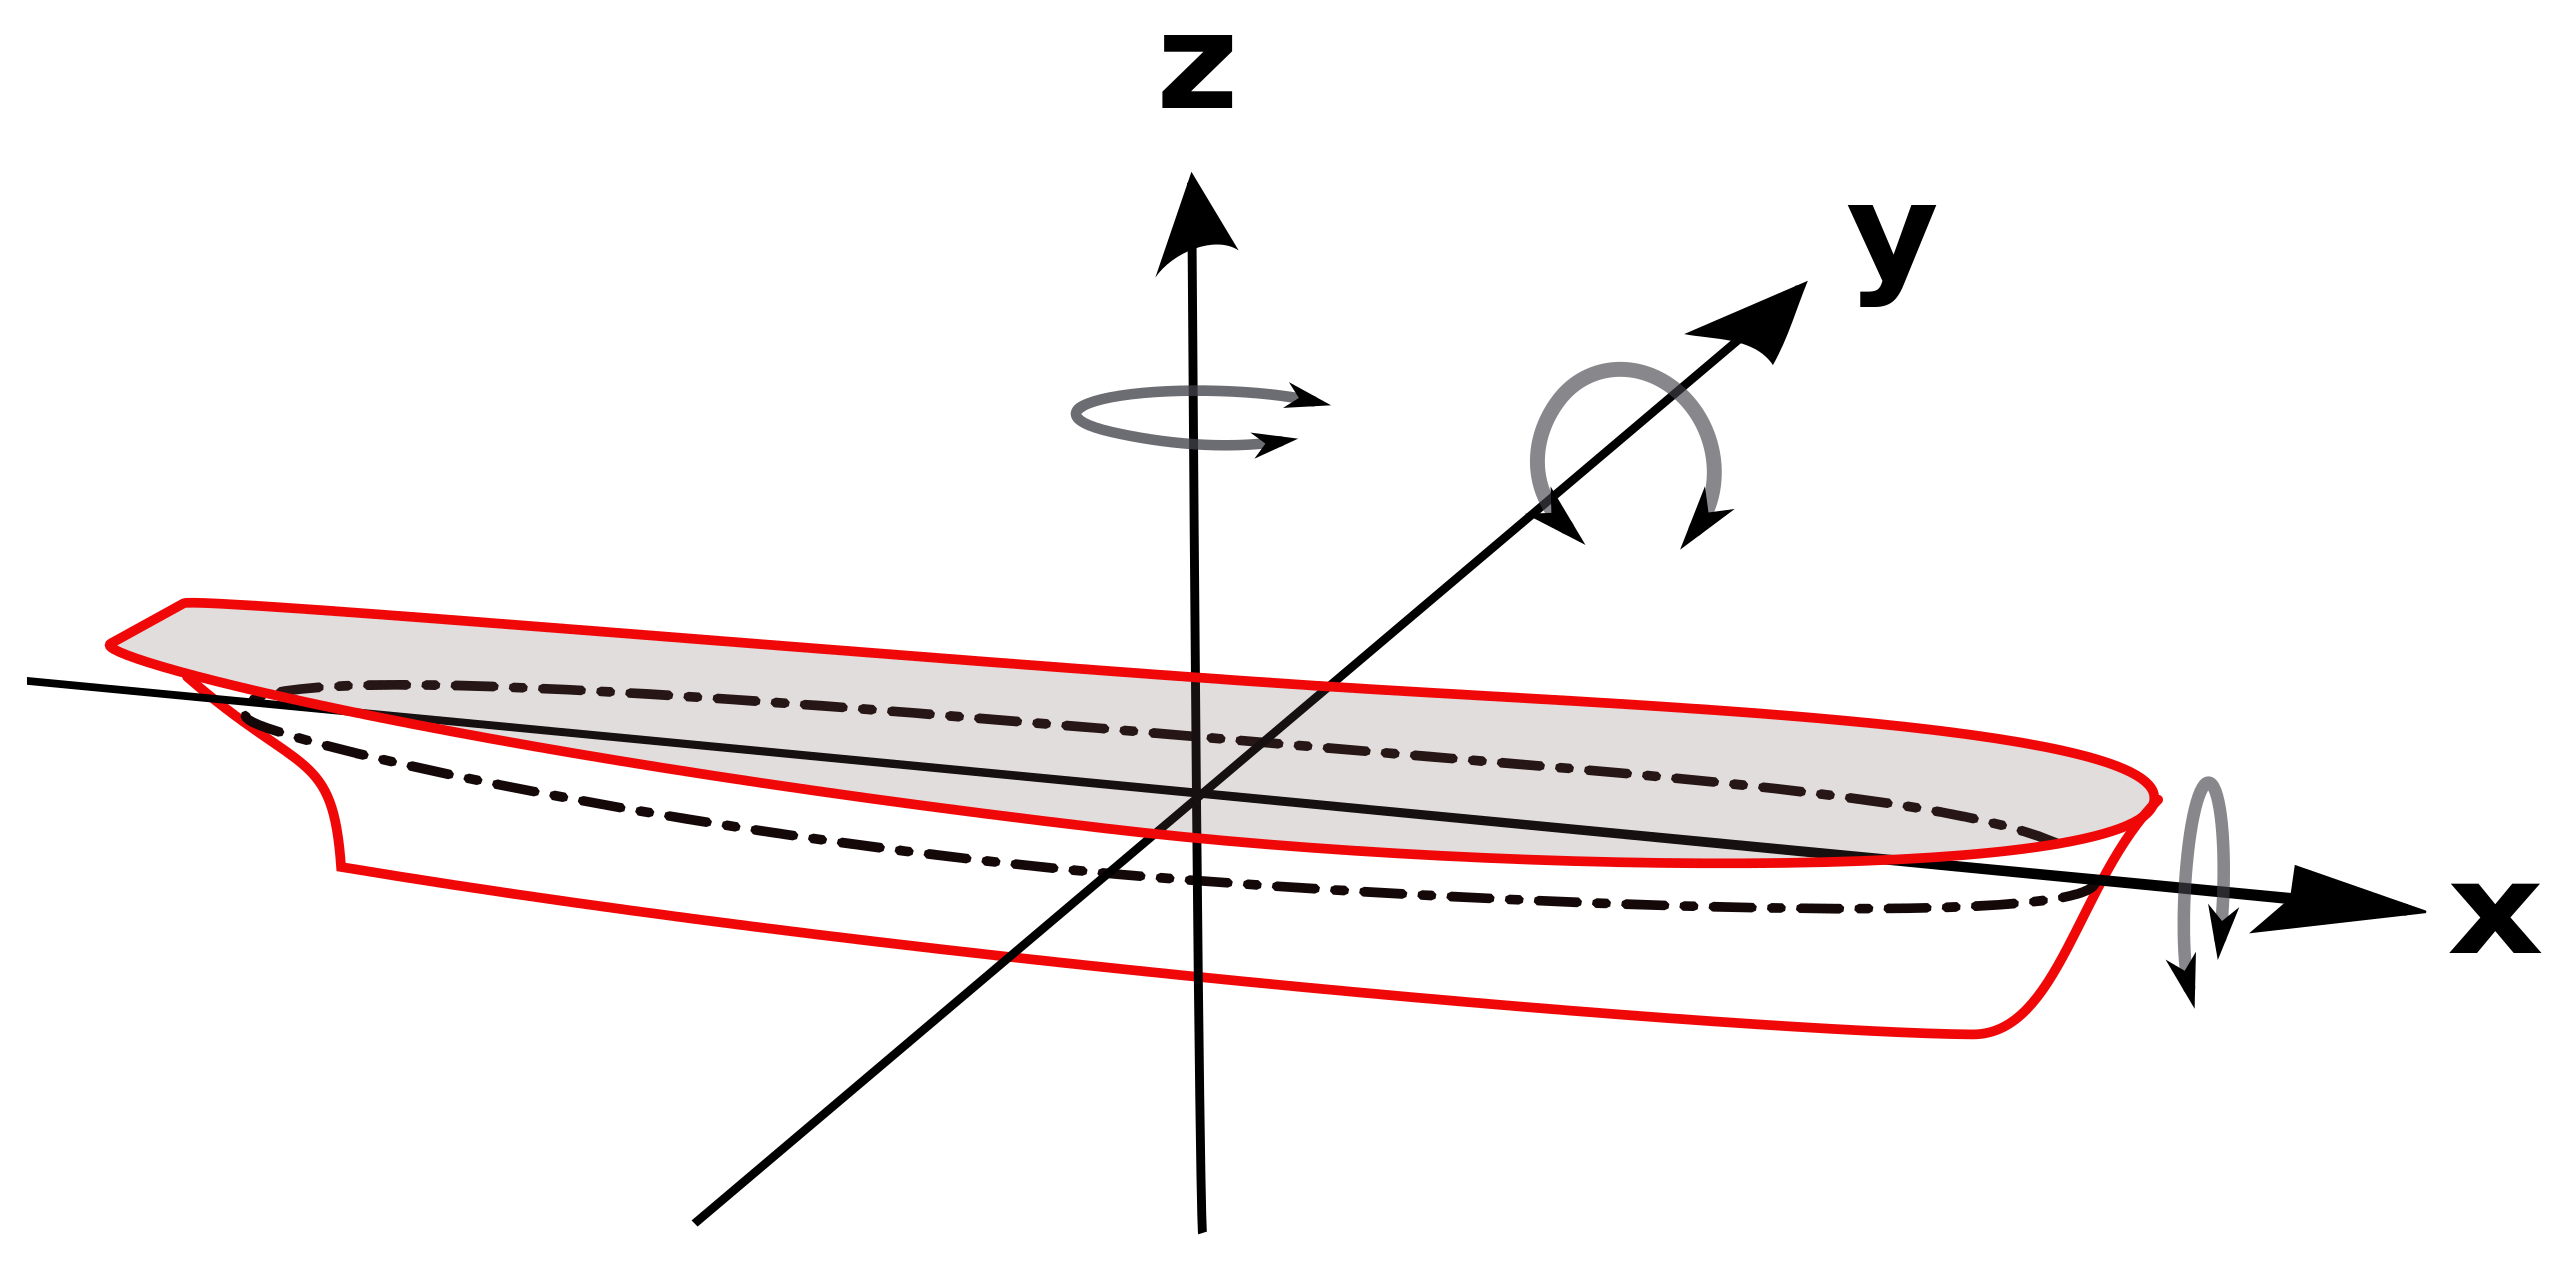
\includegraphics[width=0.5\linewidth]{assets/Achsen_Schiffsbewegung.svg.png}
    \caption{Krängung}
    \label{fig:enter-label}
\end{figure}
Die Stabilität eines Bootes wird durch die drei Parameter Gewichtsschwerpunkt, Auftriebsschwerpunkt (auch Form- oder Verdrängungsschwerpunkt genannt), sowie die sich aus ihnen ergebende sogeannte metazentrische Höhe bestimmt. 
https://de.wikipedia.org/wiki/Stabilität_(Schiffskörper)

\\Der Gewichtsschwerpunkt steht für die gesamte in einem Punkt konzentrierte nach unten wirkende Gewichtskraft des Bootes. Seine Lage innerhalb des Bootes  verändert sich bei einer Krängung nicht, solange alle Massen im Boot unverändert an ihrem Ort verharren. \\
Der Auftriebsschwerpunkt steht für die gesamte in einem Punkt konzentrierte nach oben wirkende Gewichtskraft des verdrängten Wassers. Seine Lage ändert sich bei einer Krängung, weil sich durch die Rumpfform auch die „Form“ des verdrängten Wassers ändert.\\
Bei aufrechter Schwimmlage des Schiffes liegt der Gewichtsschwerpunkt exakt vertikal über dem Auftriebsschwerpunkt. Führt ein äusserer Einfluss aber zu einer Krängung des Bootes, verändert sich die Lages des  stehen Gewichtsschwerpunkt auf der horizontalen Achse. Gewichtsschwerpunkt und Auftriebsschwerpunkt stehen  damit nicht mehr senkrecht übereinander. Dadurch entsteht ein aufrichtendes Drehmoment, welches das Boot bei Wegfall des krängenden Einflusses in seine Ausgangslage zurückführt. 
\begin{figure}
    \centering
    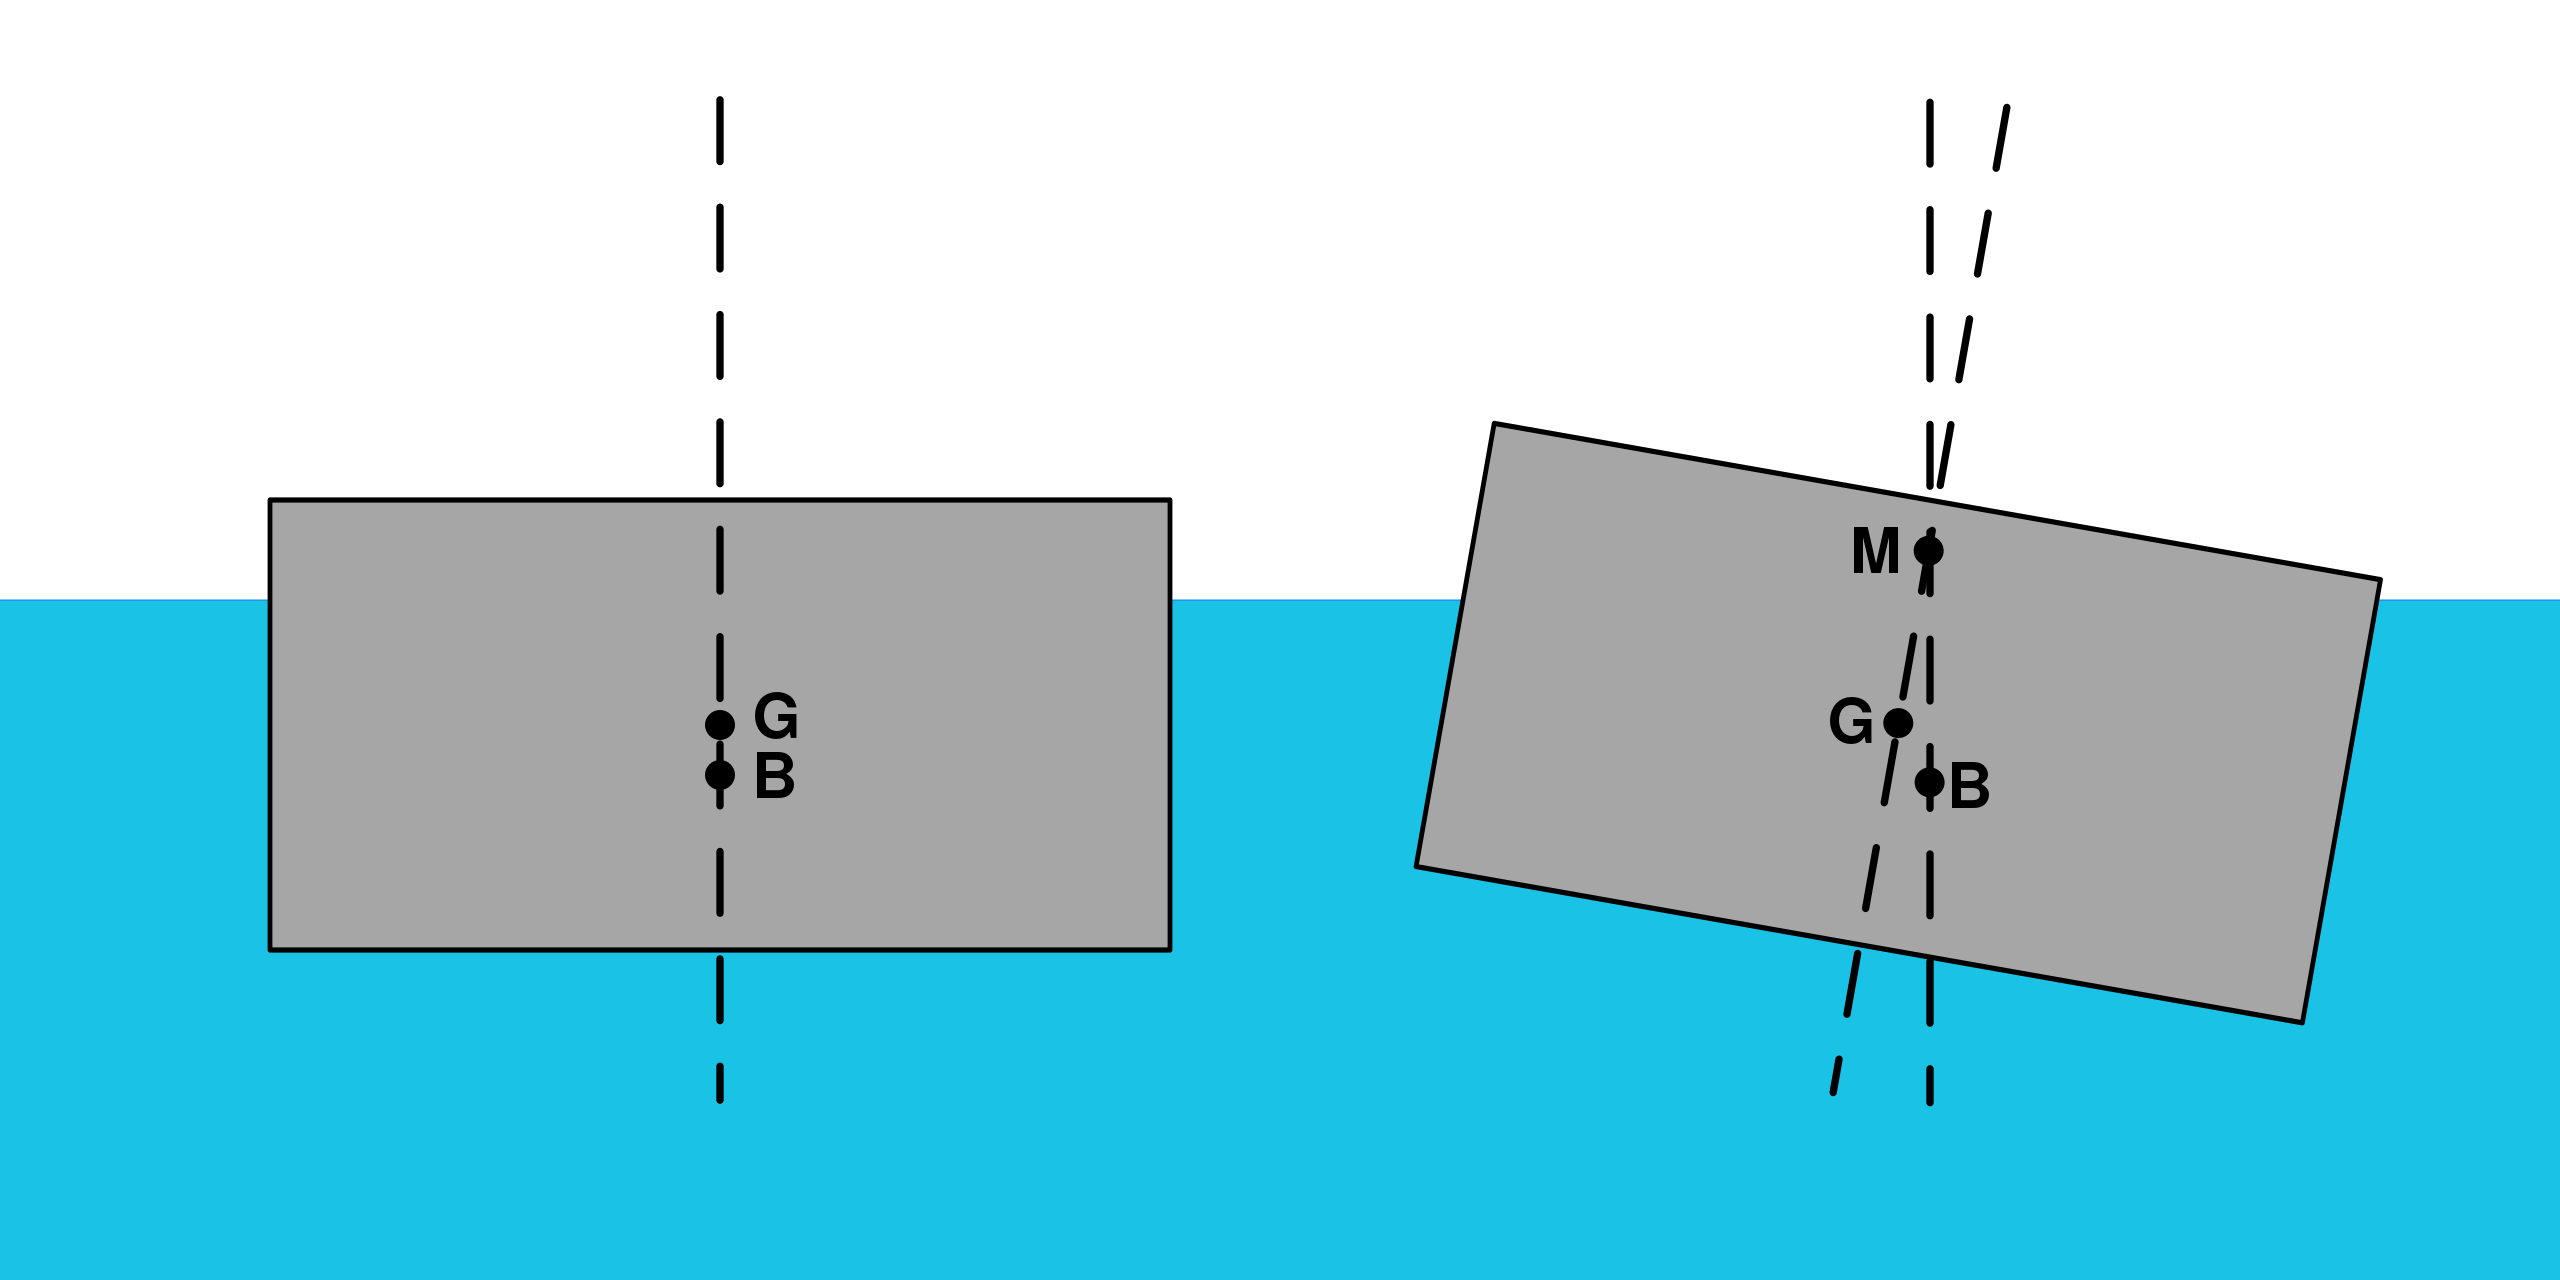
\includegraphics[width=0.5\linewidth]{Metacentriskhojd-svg.svg.png}
    \caption{Lage des Gewichtsschwerpunkt (G), Auftriebsschwerpunkt (B) und Metazentrum (M) bei aufrechtem, sowie gekrängtem Boot }
    \label{fig:enter-label}
\end{figure}
Zur Bewertung der Stabilität eines Schiffes müssen die folgenden drei Parameter bekannt sein: (i) die Anfangsstabilität (die sogeannte metazentrische Anfangshöhe), (ii) der Stabilitätsumfang und (iii) die Fläche unter der Hebelarmkurve. Die metazentrische Höhe ist der Parameter für den aufrichtenden Hebelarm. Mit dem Stabilitätsumfang wird die rechnerische Krängung des Schiffes in Winkelgraden bis zum Kenterpunkt bezeichnet und mit der Hebelarmkurve wird der jeweilige aufrichtende Hebelarm über den vollen Krängungsbereich bis zum Kenterpunkt des Bootes grafisch dargestellt. Der Hebelarm wächst bei zunehmender Krängung zunächst steil an, dann immer flacher an und wird bei noch stärkerer Krängung wieder geringer, bis er schließlich den Kenterpunkt (C) erreicht. Dieser liegt da, wo der Gewichtsschwerpunkt über den Auftriebsschwerpunkt hinauswandert. Mit der Fläche unter der Hebelarmkurve (A) lässt sich die Erfüllung der geplanten Mindeststabilität belegen.  https://de.wikipedia.org/wiki/Stabilit%C3%A4t_(Schiffsk%C3%B6rper))

\begin{figure}
    \centering
    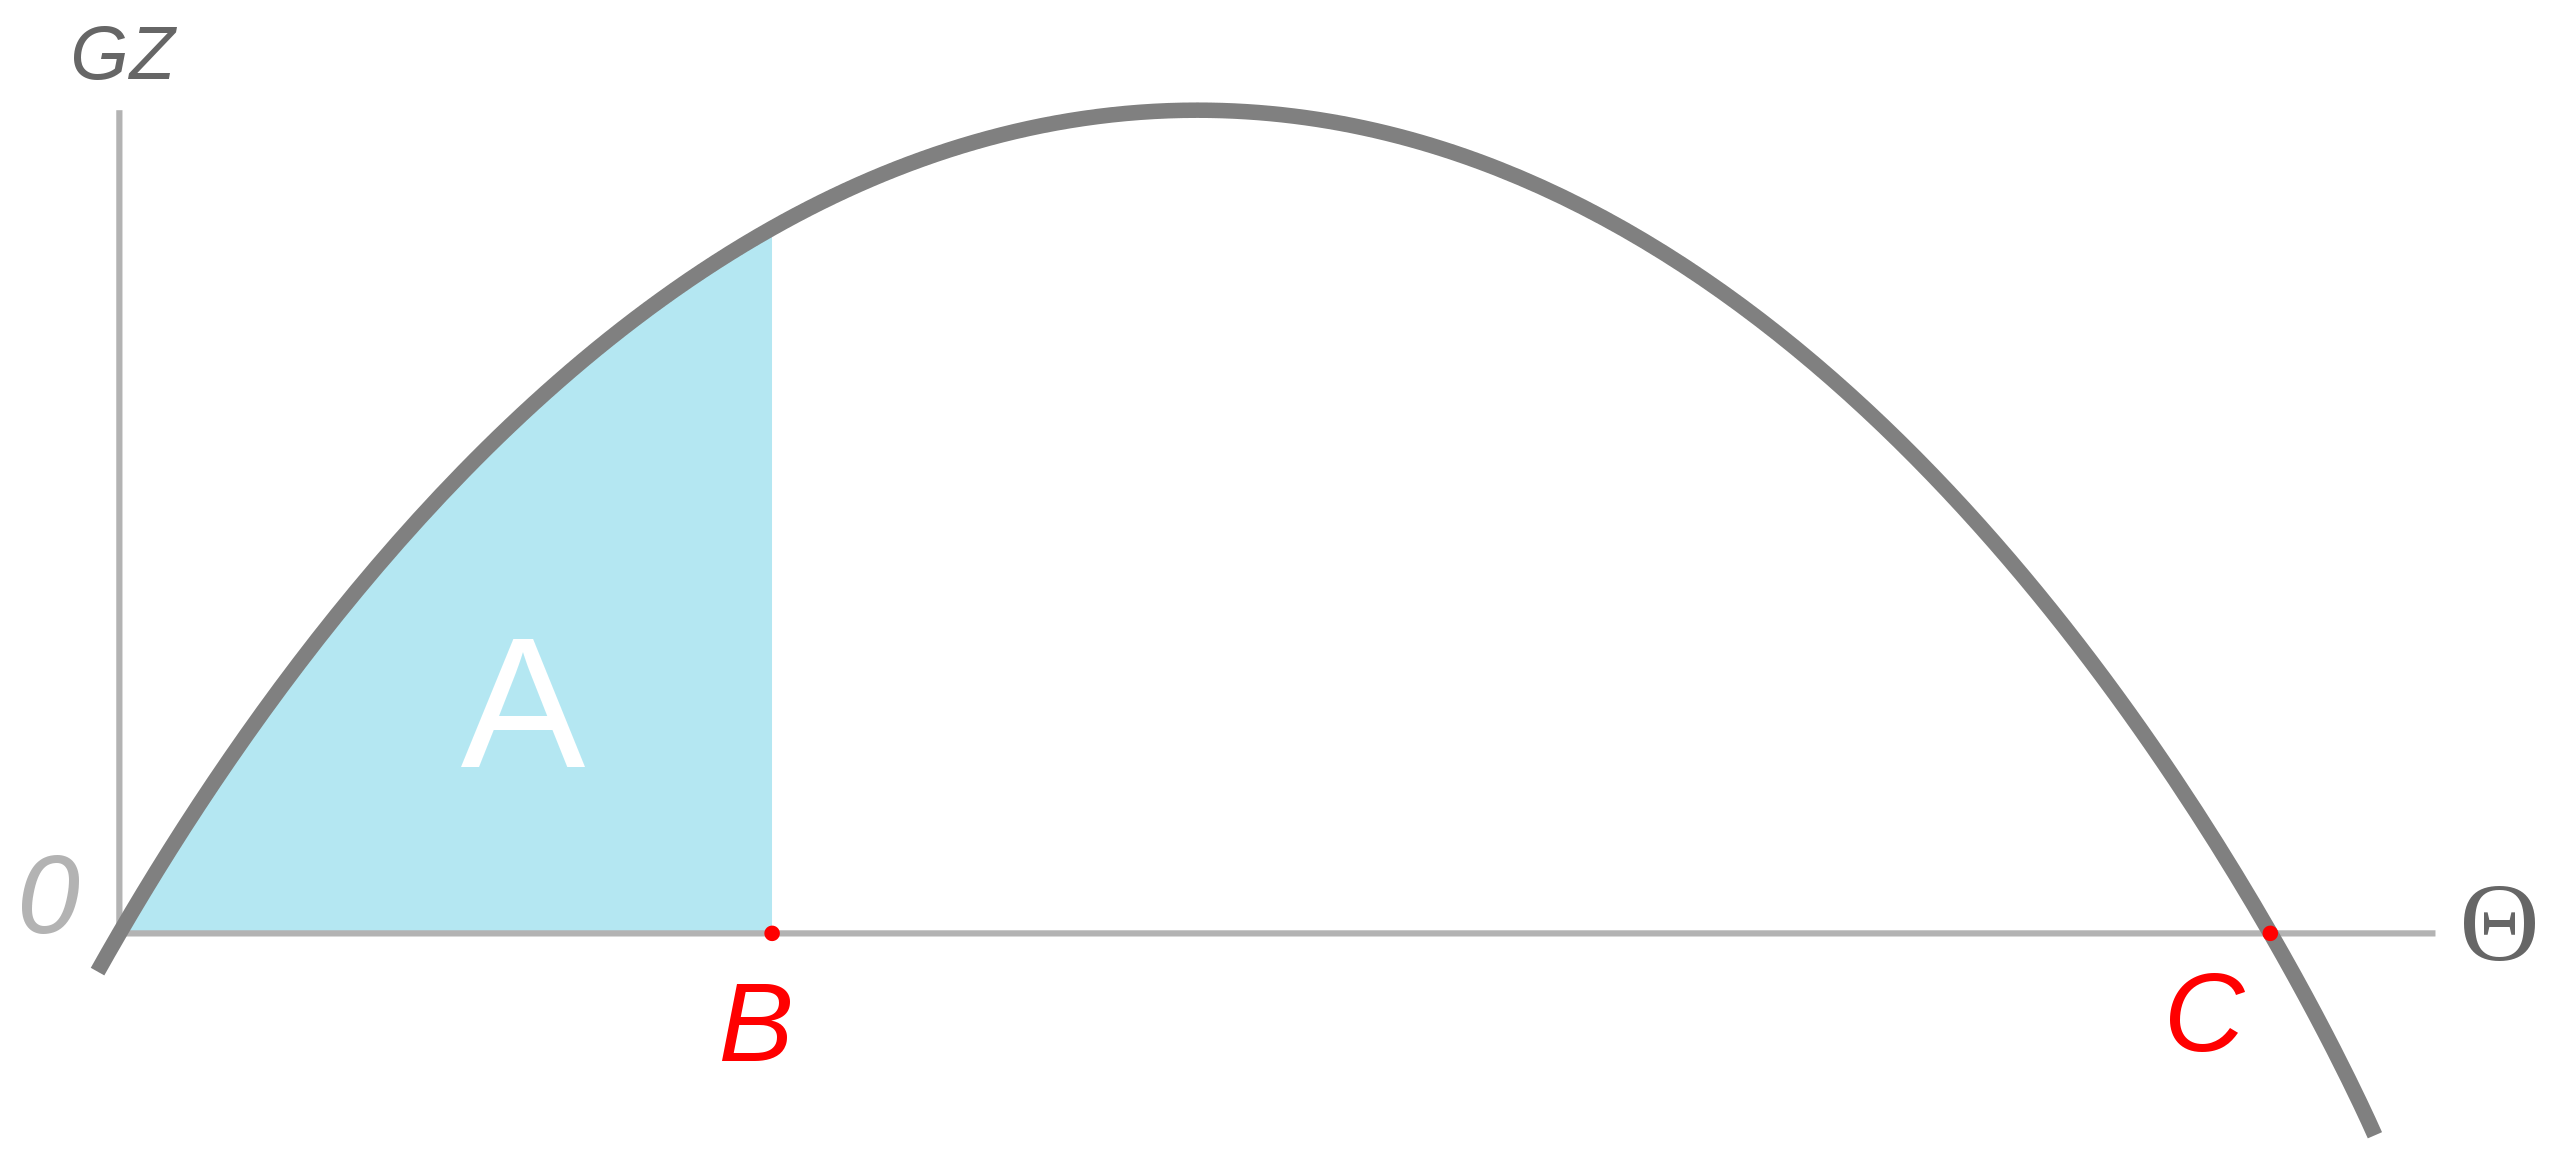
\includegraphics[width=0.5\linewidth]{Stability_curve_NT.svg.png}
    \caption{Hebelarmkurve}
    \label{fig:enter-label}
\end{figure}
Bei Segelbooten sind die Überlegungen zur Stabilität besonders wichtig, da sie mit ihren Segel für den Wind eine sehr grosse Angriffsfläche bieten. Ohne geeignete Gegenmassnahmen kippen sie schon bei geringen Windstärken um. Entscheidnd für die Stabilität eines Segelbootes sind dabei die Rumpfform und Gewichtsverteilung des Bootes. Die Krängung kann durch zwei Massnahmen wieder ausgeglichen und damit die Stabilität erhöht werden: 
\begin{itemize}
    \item Gewichtsstabilität – ein tief liegender Ballastkiel zwingt das Boot wieder in die aufrechte Lage (sogenanntes Stehaufmännchen-Prinzip).
    \item Formstabilität – die Form des Rumpfes begünstigt eine Rückkehr in die Ausgangslage.
\end{itemize}

\paragraph{Gewichtsstabilität}
Gewichtsstabilität durch Ballastkiel
Bei \href{https://de.wikipedia.org/wiki/Segelschiff}{Segelschiffen} wirkt ein \href{https://de.wikipedia.org/wiki/Kiel_(Schiffbau)}{Ballastkiel} als Gegengewicht der \href{https://de.wikipedia.org/wiki/Kr\%C3\%A4ngung}{Krängung} entgegen. Dieser enthält bis zu 50 \% der Masse des Schiffes und bewirkt so ein aufrichtendes Moment. Eine gewisse Krängung unter Segeln – je nach Bauart des Schiffes von 20 bis 45° – ist bei diesen Schiffen normal und stellt keine Gefahr für das Schiff dar. Im untenstehenden Bild ist G der \textit{\href{https://de.wikipedia.org/wiki/Gewichtsschwerpunkt}{Gewichtsschwerpunkt}} (Schwerpunkt des Bootes) und A der \textit{\href{https://de.wikipedia.org/wiki/Formschwerpunkt}{Formschwerpunkt}} (Schwerpunkt der verdrängten Wassermasse). Für mechanische Betrachtungen kann man sich die Gewichtskräfte als im Punkt G vereinigt denken und die Auftriebskräfte als im Punkt A. Mit zunehmender Krängung wandert der Gewichtsschwerpunkt weiter nach außen und es erhöht sich damit das aufrichtende \href{https://de.wikipedia.org/wiki/Drehmoment}{Drehmoment}. Manche Segelschiffe richten sich daher selbst bei einer Krängung von mehr als 120° noch selbstständig wieder auf. Erst durch sehr hohen \href{https://de.wikipedia.org/wiki/Seegang}{Wellengang} können sie mit dem Kiel nach oben gedreht werden und gelten daher als \href{https://de.wikipedia.org/wiki/Kentern}{kentersicher}. Dringen allerdings größere Mengen Wasser ins Bootsinnere, sinken sie wegen des hohen Ballastgewichts. Verliert ein solcher Rumpf, beispielsweise nach einer Grundberührung, seinen Ballastkiel, so ist kaum mehr Stabilität vorhanden und das Kentern faktisch nicht mehr zu verhindern. 
\begin{figure}
    \centering
    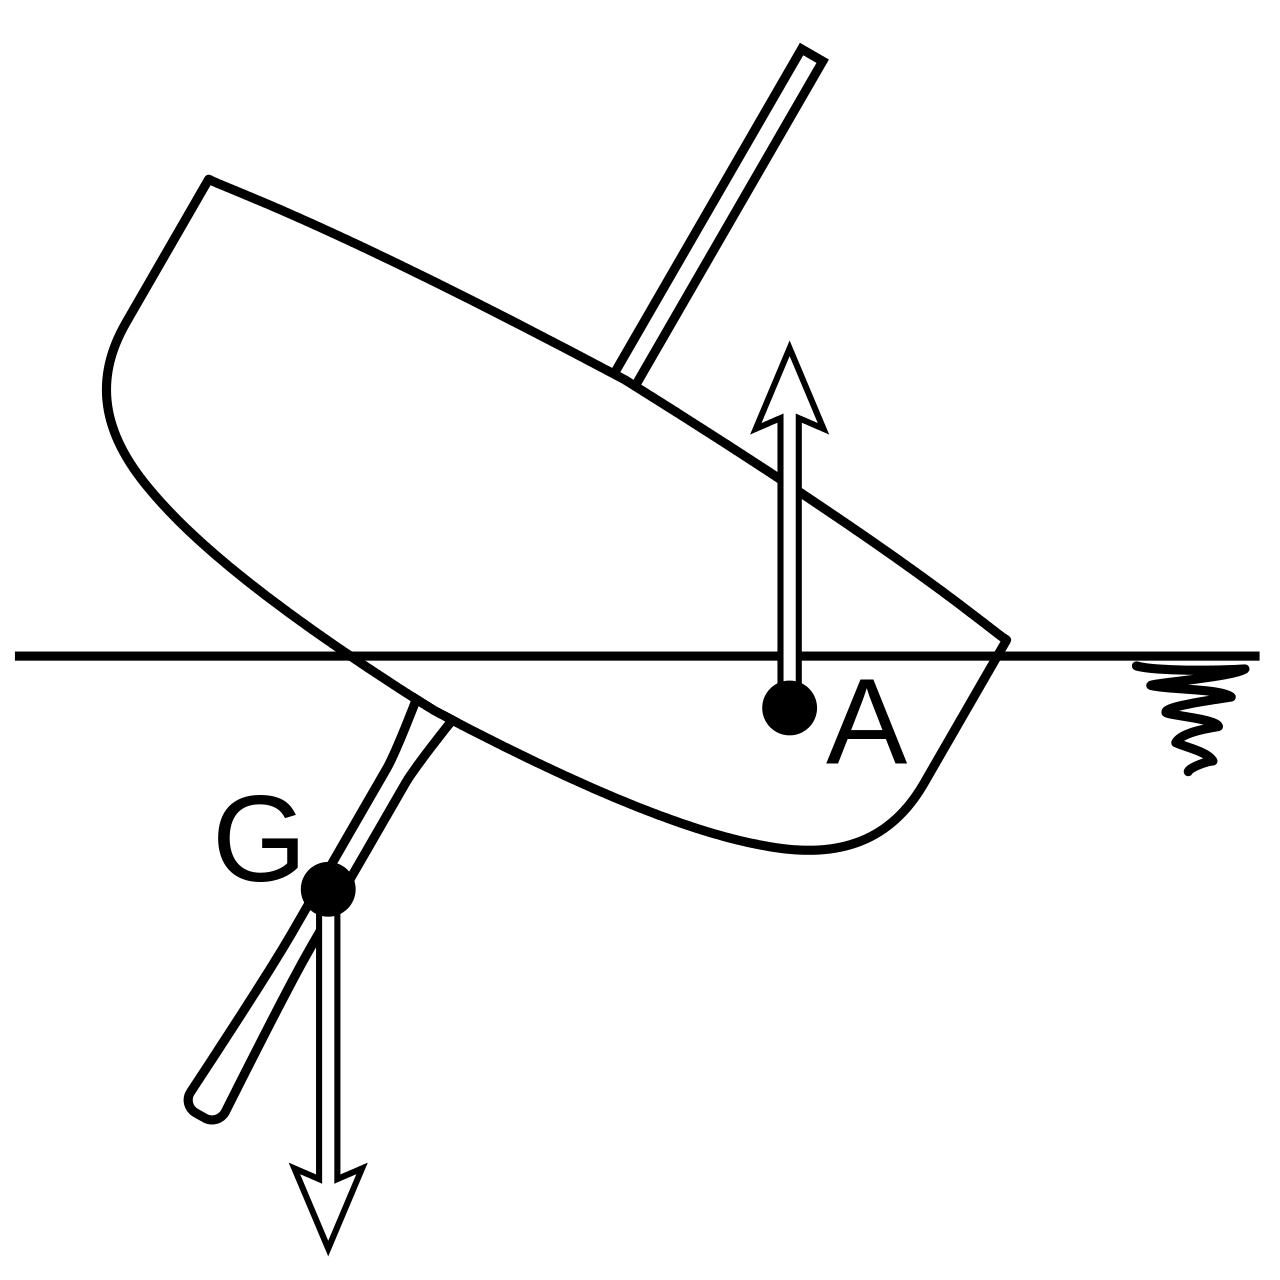
\includegraphics[width=0.5\linewidth]{Segeln_Gewichtsstabilitaet.svg.png}
    \caption{Gewichtsstabilität durch Ballastkiel }
    \label{fig:enter-label}
\end{figure}

\paragraph{Formstabilität}
Im Unterschied zu Kielyachten sind die meisten \href{https://de.wikipedia.org/wiki/Jolle}{Jollen} überwiegend formstabil. Das (meist ausklappbare) leichte Schwert einer Jolle hat keinen nennenswerten aufrichtenden Effekt. Auch \href{https://de.wikipedia.org/wiki/Segelkatamaran}{Katamarane} oder \href{https://de.wikipedia.org/wiki/Trimaran}{Trimarane} haben aufgrund ihrer Breite eine hohe Formstabilität. 
Im untenstehenden Bild ist G der Gewichtsschwerpunkt (Schwerpunkt des Bootes) und A der Formschwerpunkt (Schwerpunkt der verdrängten Wassermasse). In diesen Punkten kann man sich die Gewichts- bzw. Auftriebskräfte vereinigt denken. Für die Formstabilität ist die Lage von A ausschlaggebend. 

Bei aufrechter Lage des Bootes wird auf beiden Seiten des Rumpfes gleich viel Wasser verdrängt. A befindet sich dann mittig im Rumpfquerschnitt, es entsteht kein Drehmoment. Mit zunehmender Krängung (siehe Bild) wird Wasser vor allem auf einer Seite des Rumpfes verdrängt. Dadurch wandert A nach außen, es entsteht ein Drehmoment. Je breiter das Boot ist, desto weiter wandert A nach außen und desto stärker ist das aufrichtende Drehmoment. Wenn die Krängung zu groß wird, nimmt das Drehmoment allerdings wieder ab, weil dann der breite Rumpf gekippt ist und A wieder näher zur Mitte liegt. Eine leichte Krängung wird daher durch das kräftige aufrichtende Drehmoment kompensiert („Wasserwiderstand“), während eine zu starke Krängung zum Kentern des Bootes führt. Katamarane kentern, wenn die Krängung 90° erreicht.\textsuperscript{\href{https://de.wikipedia.org/wiki/Stabilit\%C3\%A4t_(Schiffsk\%C3\%B6rper)\#cite_note-Seemannschaft,_Seite_163-1}{[1]}} 

Es gibt sogar Beispiele für komplett formstabile Bootstypen mit negativer Anfangsstabilität. Diese haben im Ruhezustand keine aufrechte Schwimmlage. 
\begin{figure}
    \centering
    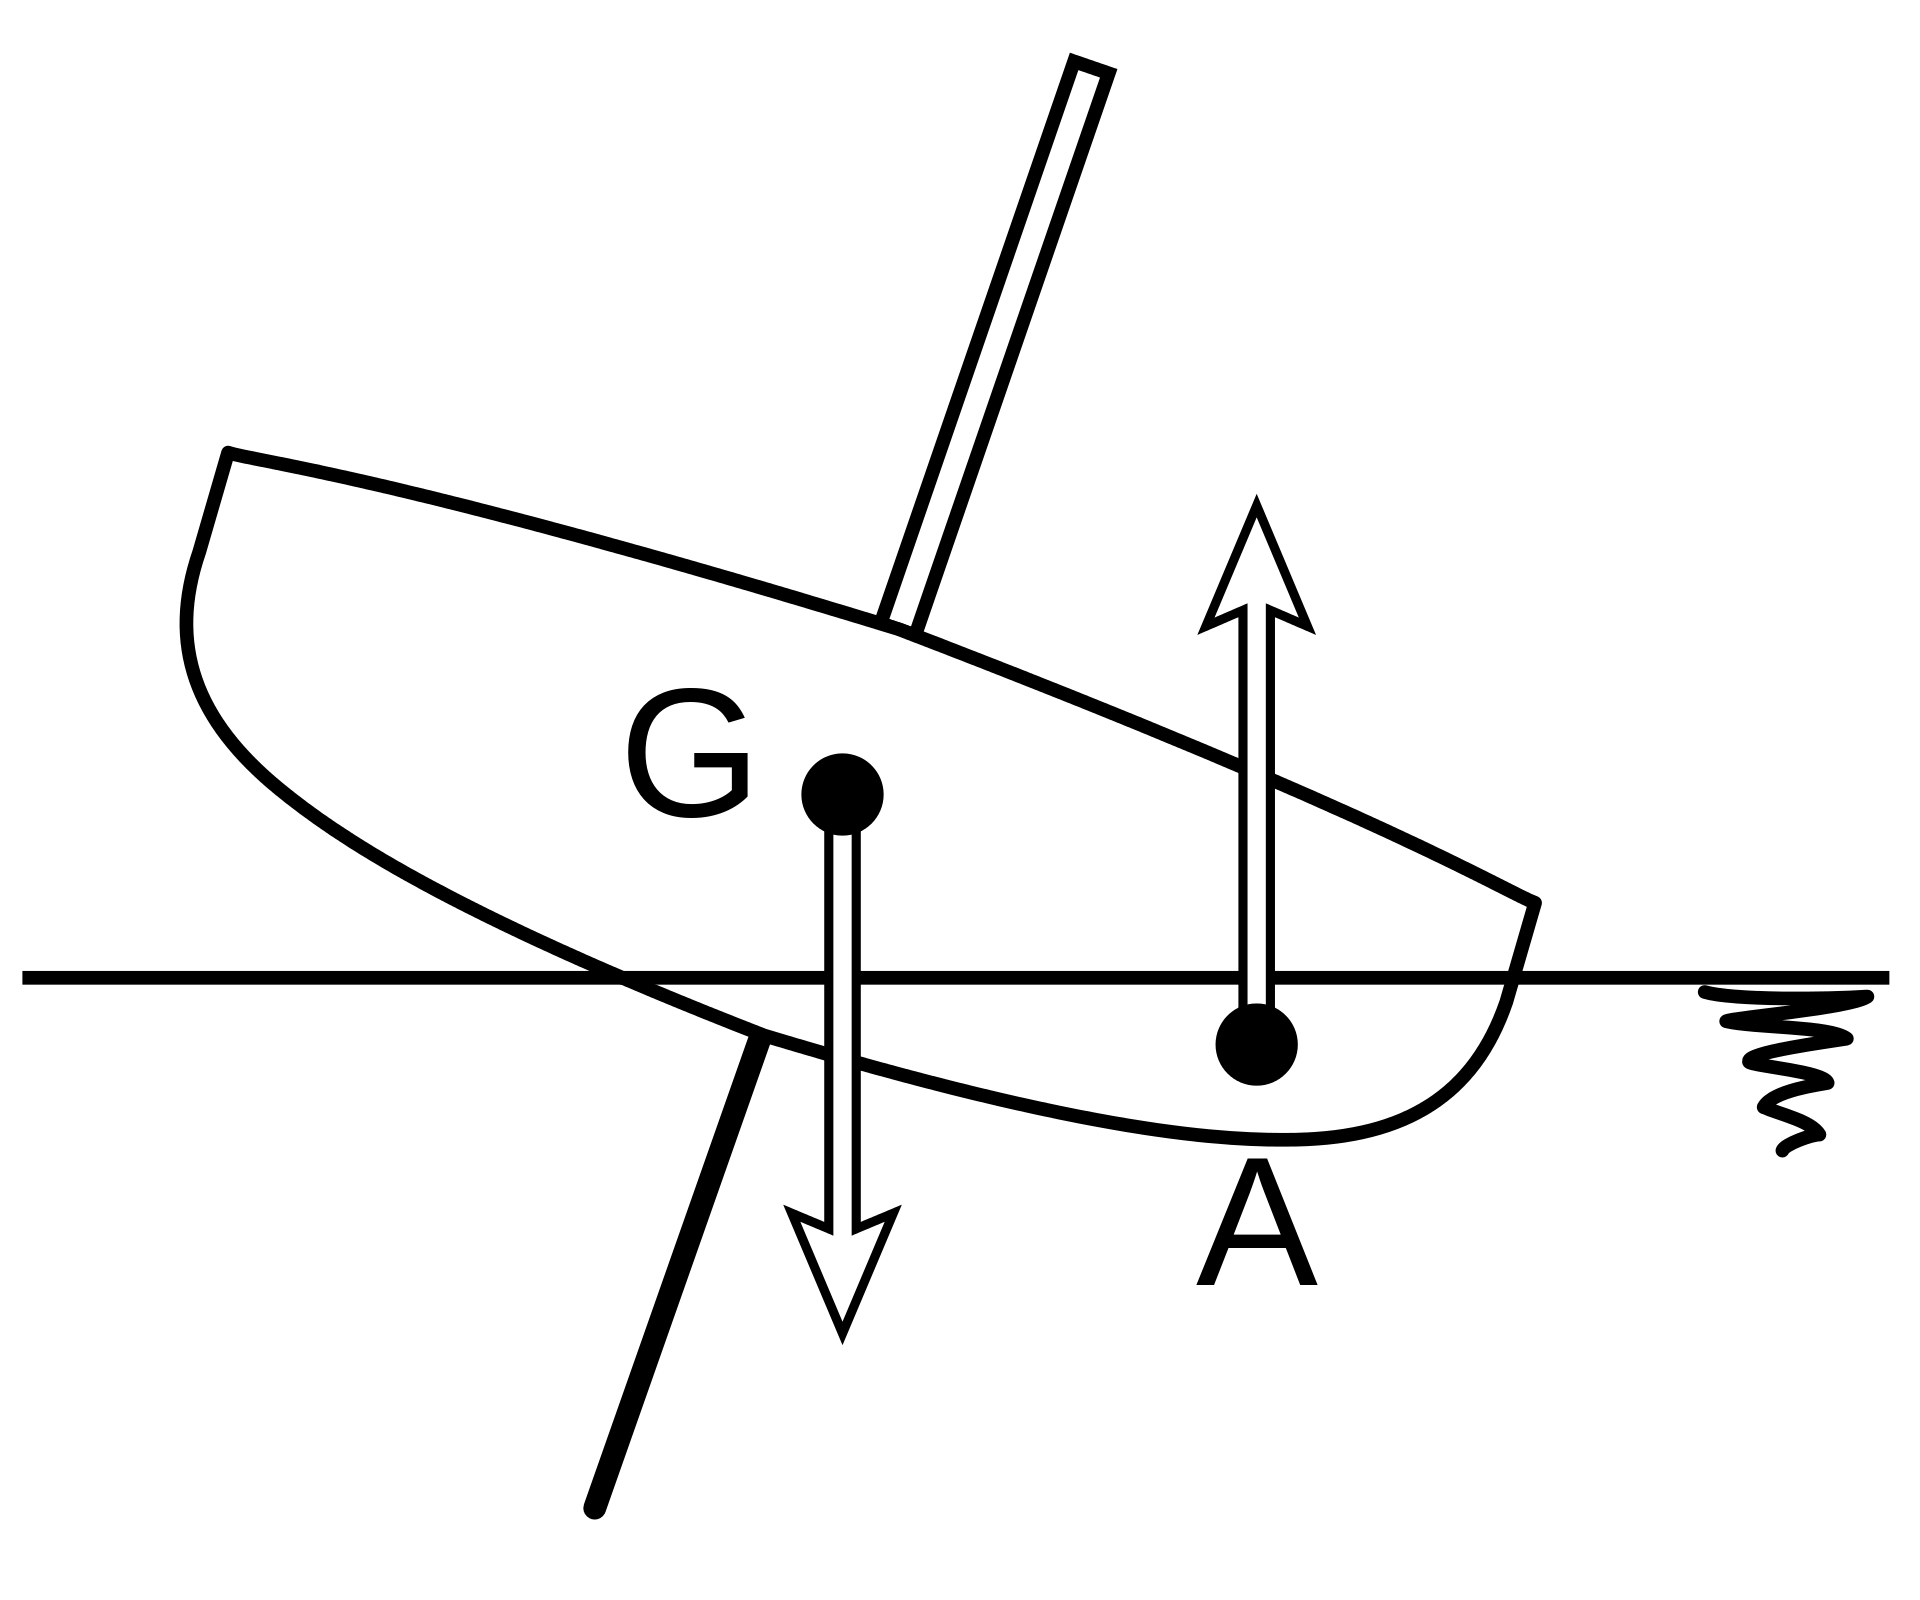
\includegraphics[width=0.5\linewidth]{Segeln_Formstabilitaet.svg.png}
    \caption{Formstabilität }
    \label{fig:enter-label}
\end{figure}

\paragraph{Gegenmaßnahmen bei großer Krängung}

Ein Segler hängt im Trapez, um den Katamaran auszubalancieren.Sowohl bei Kielbooten als auch bei Katamaranen oder Jollen kann die Krängung reduziert werden, indem sich die Crew „auf die hohe Kante setzt“, das heißt sich im \href{https://de.wikipedia.org/wiki/Luv_und_Lee}{Luv} an die Reling setzt, oder die Segelfläche reduziert wird (\href{https://de.wikipedia.org/wiki/Reffen}{Reffen}). Bei sportlich gesegelten \href{https://de.wikipedia.org/wiki/Jolle}{Jollen} hängt sich die Crew in ein \href{https://de.wikipedia.org/wiki/Trapez_(Segeln)}{Trapez}, um weiter nach Luv ausreiten zu können.\textsuperscript{\href{https://de.wikipedia.org/wiki/Stabilit\%C3\%A4t_(Schiffsk\%C3\%B6rper)\#cite_note-2}{[2]}} Beim sportlichen Segeln von Jollen kann eine Kenterung schon mal vorkommen. Sie sind im Gegenzug mit Schwimmkörpern ausgerüstet, so dass sie trotz Kenterung nicht sinken. Jollen sind dennoch nicht für die Hochsee geeignet und selbst gute Jollensegler werden bei angekündigten \href{https://de.wikipedia.org/wiki/Beaufort-Skala}{Windstärken} von mehr als 6 nicht mehr ablegen. 

Durch die Krängung wird automatisch die wirksame Segelfläche reduziert, auch die Form des Rumpfes bevorzugt einen bestimmten Krängungswinkel, bei dem das Schiff die höchste Geschwindigkeit erreichen kann. Daher wird durch starke Krängung das Schiff langsamer, zudem wird der Aufenthalt an Bord ungemütlicher. Auch steigt die Gefahr, dass es durch zu starke Krängung zu einem sogenannten \href{https://de.wikipedia.org/wiki/Sonnenschuss}{Sonnenschuss} kommt und das Schiff „aus dem Ruder läuft“\textsuperscript{\href{https://de.wikipedia.org/wiki/Stabilit\%C3\%A4t_(Schiffsk\%C3\%B6rper)\#cite_note-3}{[3]}} und „in den Wind schießt“.\textsuperscript{\href{https://de.wikipedia.org/wiki/Stabilit\%C3\%A4t_(Schiffsk\%C3\%B6rper)\#cite_note-4}{[4]}} Noch schlimmer ist es, wenn die Nock des \href{https://de.wikipedia.org/wiki/Baum_(Segeln)}{Großbaums} ins Wasser eintaucht, was zu schweren Schäden am \href{https://de.wikipedia.org/wiki/Takelage}{Rigg} führen kann. Daher kann durch rechtzeitiges Reffen – trotz verkleinerter Segelfläche – die Geschwindigkeit zunehmen. 

 Schwertboote haben \href{https://de.wikipedia.org/wiki/Formstabilit\%C3\%A4t}{formstabile} \href{https://de.wikipedia.org/wiki/Schiffsrumpf}{Rümpfe}. Ihr aufrichtendes \href{https://de.wikipedia.org/wiki/Drehmoment}{Drehmoment} wird nicht wie bei \href{https://de.wikipedia.org/wiki/Kielboot}{Kielbooten} durch einen \href{https://de.wikipedia.org/wiki/Kiel_(Schiffbau)\#Flossenkiel}{Ballastkiel}, sondern durch entsprechende Formgebung des Rumpfquerschnittes erreicht. Schwertboote sind im Allgemeinen relativ breit. Die \href{https://de.wikipedia.org/wiki/Schiffsmast}{Masthöhe} und die gefahrene \href{https://de.wikipedia.org/wiki/Segelfl\%C3\%A4che}{Segelfläche} sind im Verhältnis zur Rumpfgröße geringer als bei Kielbooten. Schwertboote besitzen bei leichter \href{https://de.wikipedia.org/wiki/Kr\%C3\%A4ngung}{Krängung} (Neigung) ein sehr hohes aufrichtendes Moment aufgrund ihrer Formstabilität. Dieses aufrichtende Moment nimmt jedoch mit zunehmender Krängung stark ab, so dass es zur \href{https://de.wikipedia.org/wiki/Kenterung}{Kenterung} kommen kann. Bei Kielbooten ist es umgekehrt, bei leichter Krängung ist das aufrichtende Moment gering und nimmt bei zunehmender Krängung zu, sodass sie kaum kentern können bzw. sich nach einer Kenterung von alleine wieder aufrichten.  (https://de.wikipedia.org/wiki/Schwertboot)

 

Stabilität
Der Begriff Stabilität steht im Schiffbau für die Eigenschaft eines Bootes eine aufrechte Schwimmlage einzunehmen und beizubehalten oder sich selbständig wieder aufzurichten, wenn ein krängendes Drehmoment auf das Boot einwirkt oder einwirkte. Krängung ist die Neigung eines Schiffes um seine Längsachse. (https://de.wikipedia.org/wiki/Stabilit%C3%A4t_(Schiffsk%C3%B6rper)).
\begin{figure}
    \centering
    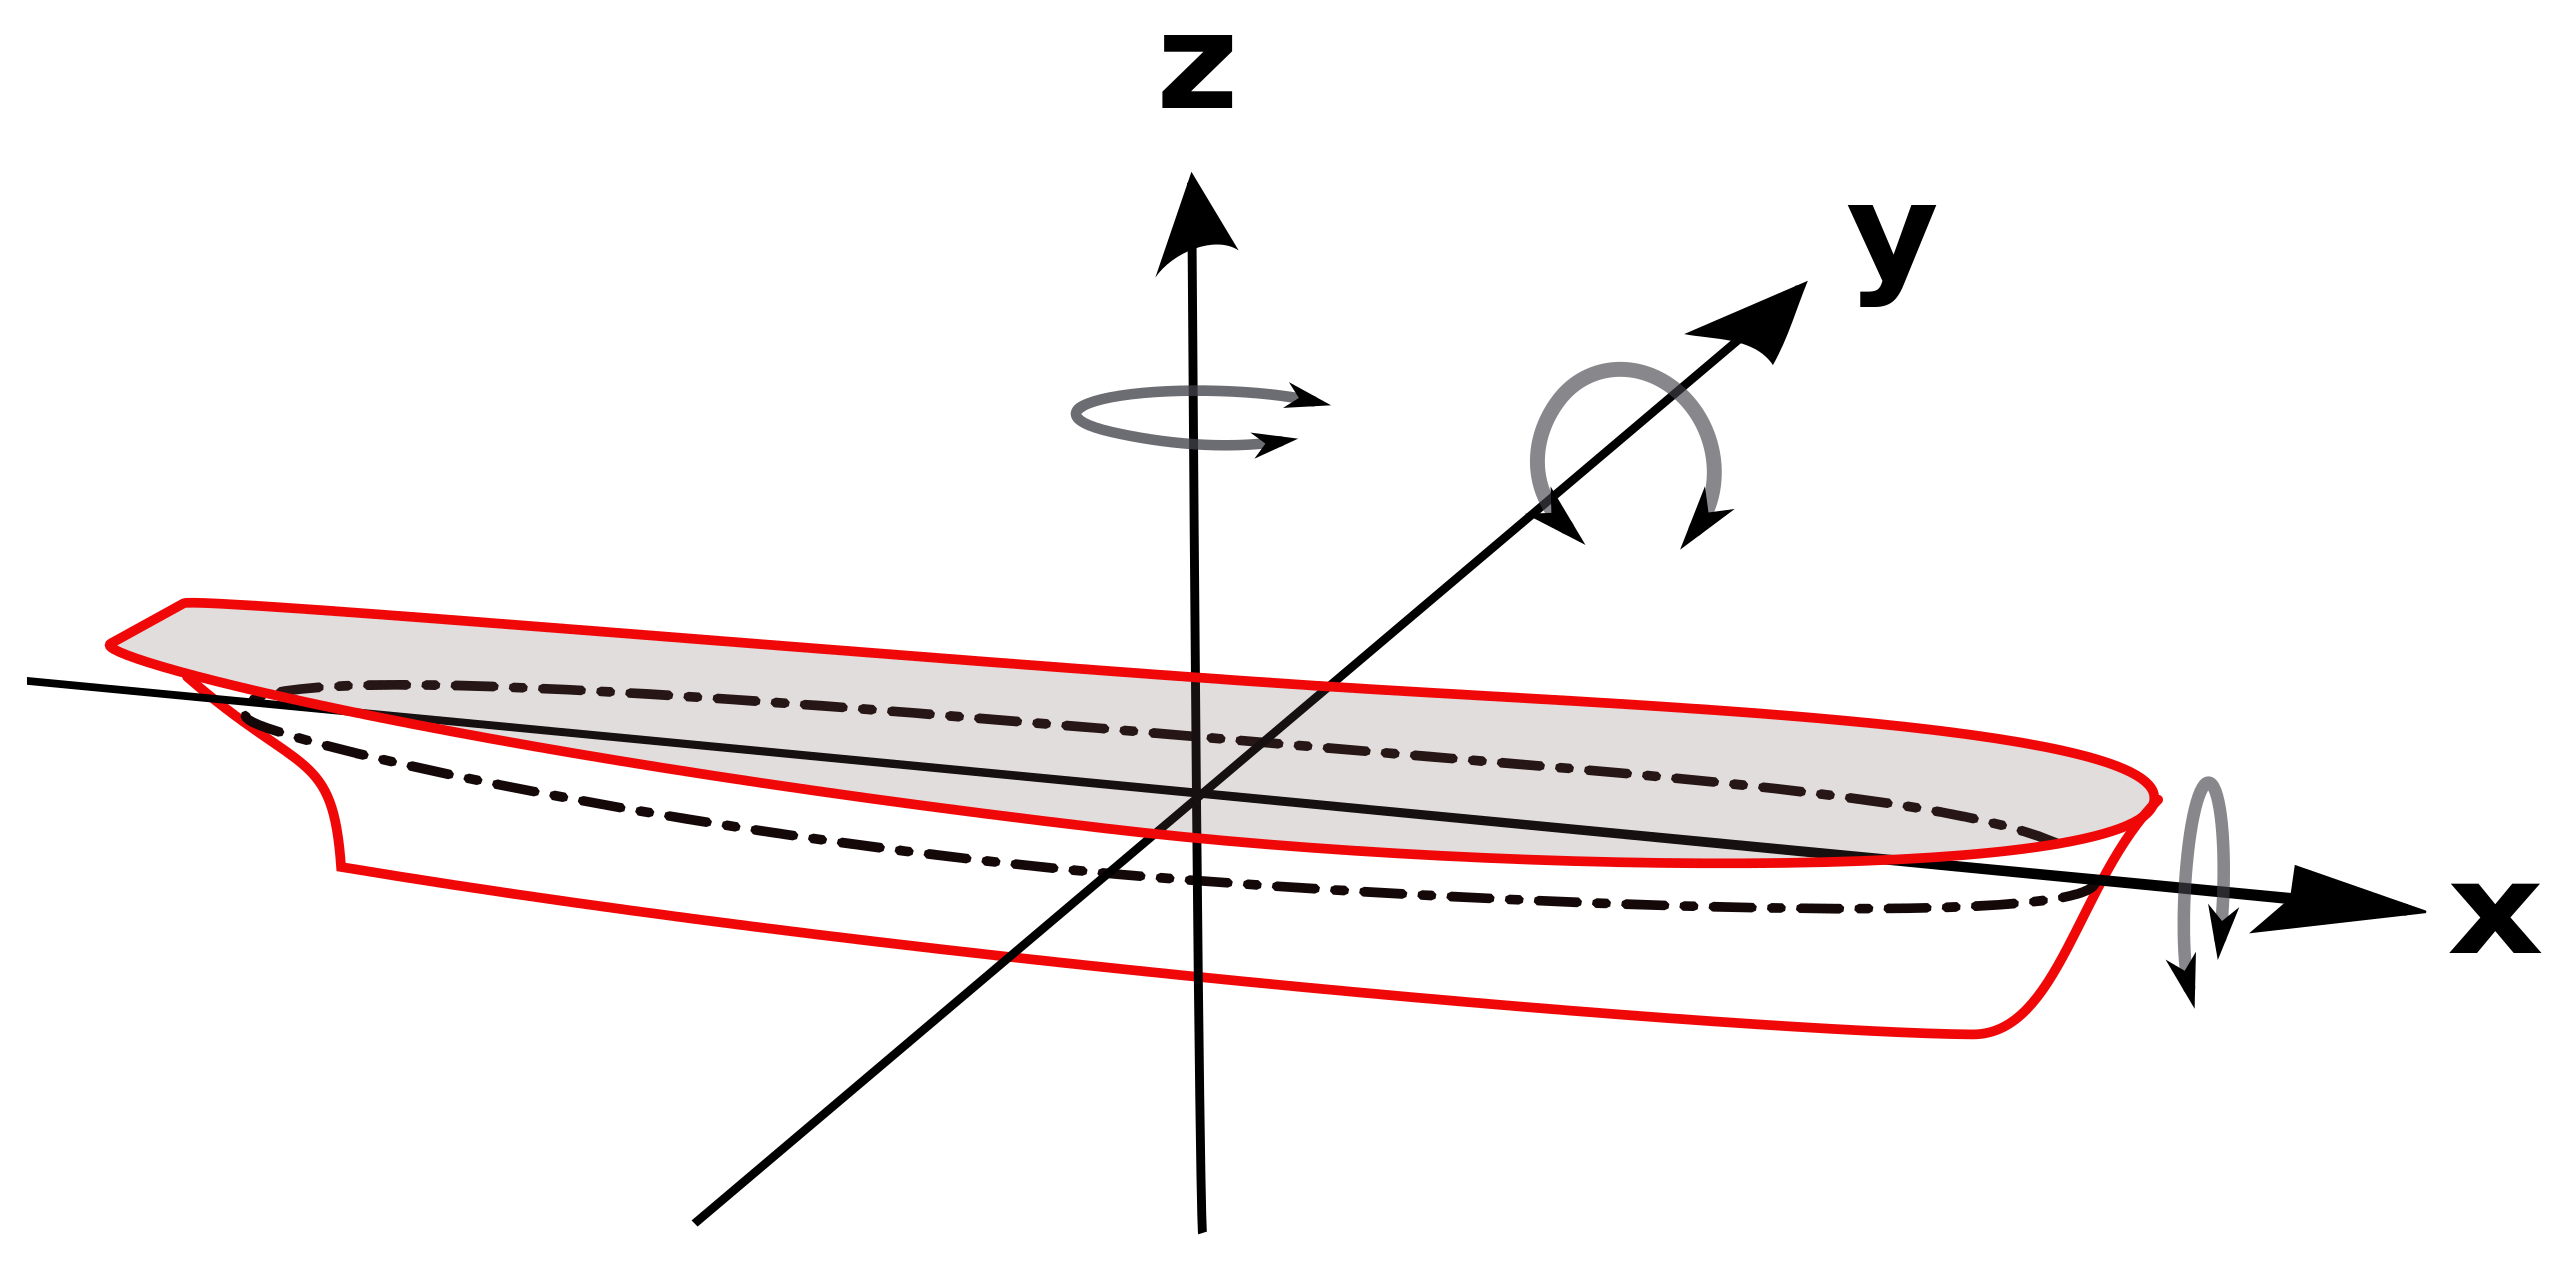
\includegraphics[width=0.5\linewidth]{assets/Achsen_Schiffsbewegung.svg.png}
    \caption{Krängung}
    \label{fig:enter-label}
\end{figure}
Die Stabilität eines Bootes wird durch die drei Parameter Gewichtsschwerpunkt, Auftriebsschwerpunkt (auch Form- oder Verdrängungsschwerpunkt genannt), sowie die sich aus ihnen ergebende sogeannte metazentrische Höhe bestimmt. (https://de.wikipedia.org/wiki/Stabilit%C3%A4t_(Schiffsk%C3%B6rper))  
\\Der Gewichtsschwerpunkt steht für die gesamte in einem Punkt konzentrierte nach unten wirkende Gewichtskraft des Bootes. Seine Lage innerhalb des Bootes  verändert sich bei einer Krängung nicht, solange alle Massen im Boot unverändert an ihrem Ort verharren. \\
Der Auftriebsschwerpunkt steht für die gesamte in einem Punkt konzentrierte nach oben wirkende Gewichtskraft des verdrängten Wassers. Seine Lage ändert sich bei einer Krängung, weil sich durch die Rumpfform auch die „Form“ des verdrängten Wassers ändert.\\
Bei aufrechter Schwimmlage des Schiffes liegt der Gewichtsschwerpunkt exakt vertikal über dem Auftriebsschwerpunkt. Führt ein äusserer Einfluss aber zu einer Krängung des Bootes, verändert sich die Lages des  stehen Gewichtsschwerpunkt auf der horizontalen Achse. Gewichtsschwerpunkt und Auftriebsschwerpunkt stehen  damit nicht mehr senkrecht übereinander. Dadurch entsteht ein aufrichtendes Drehmoment, welches das Boot bei Wegfall des krängenden Einflusses in seine Ausgangslage zurückführt. 
\begin{figure}
    \centering
    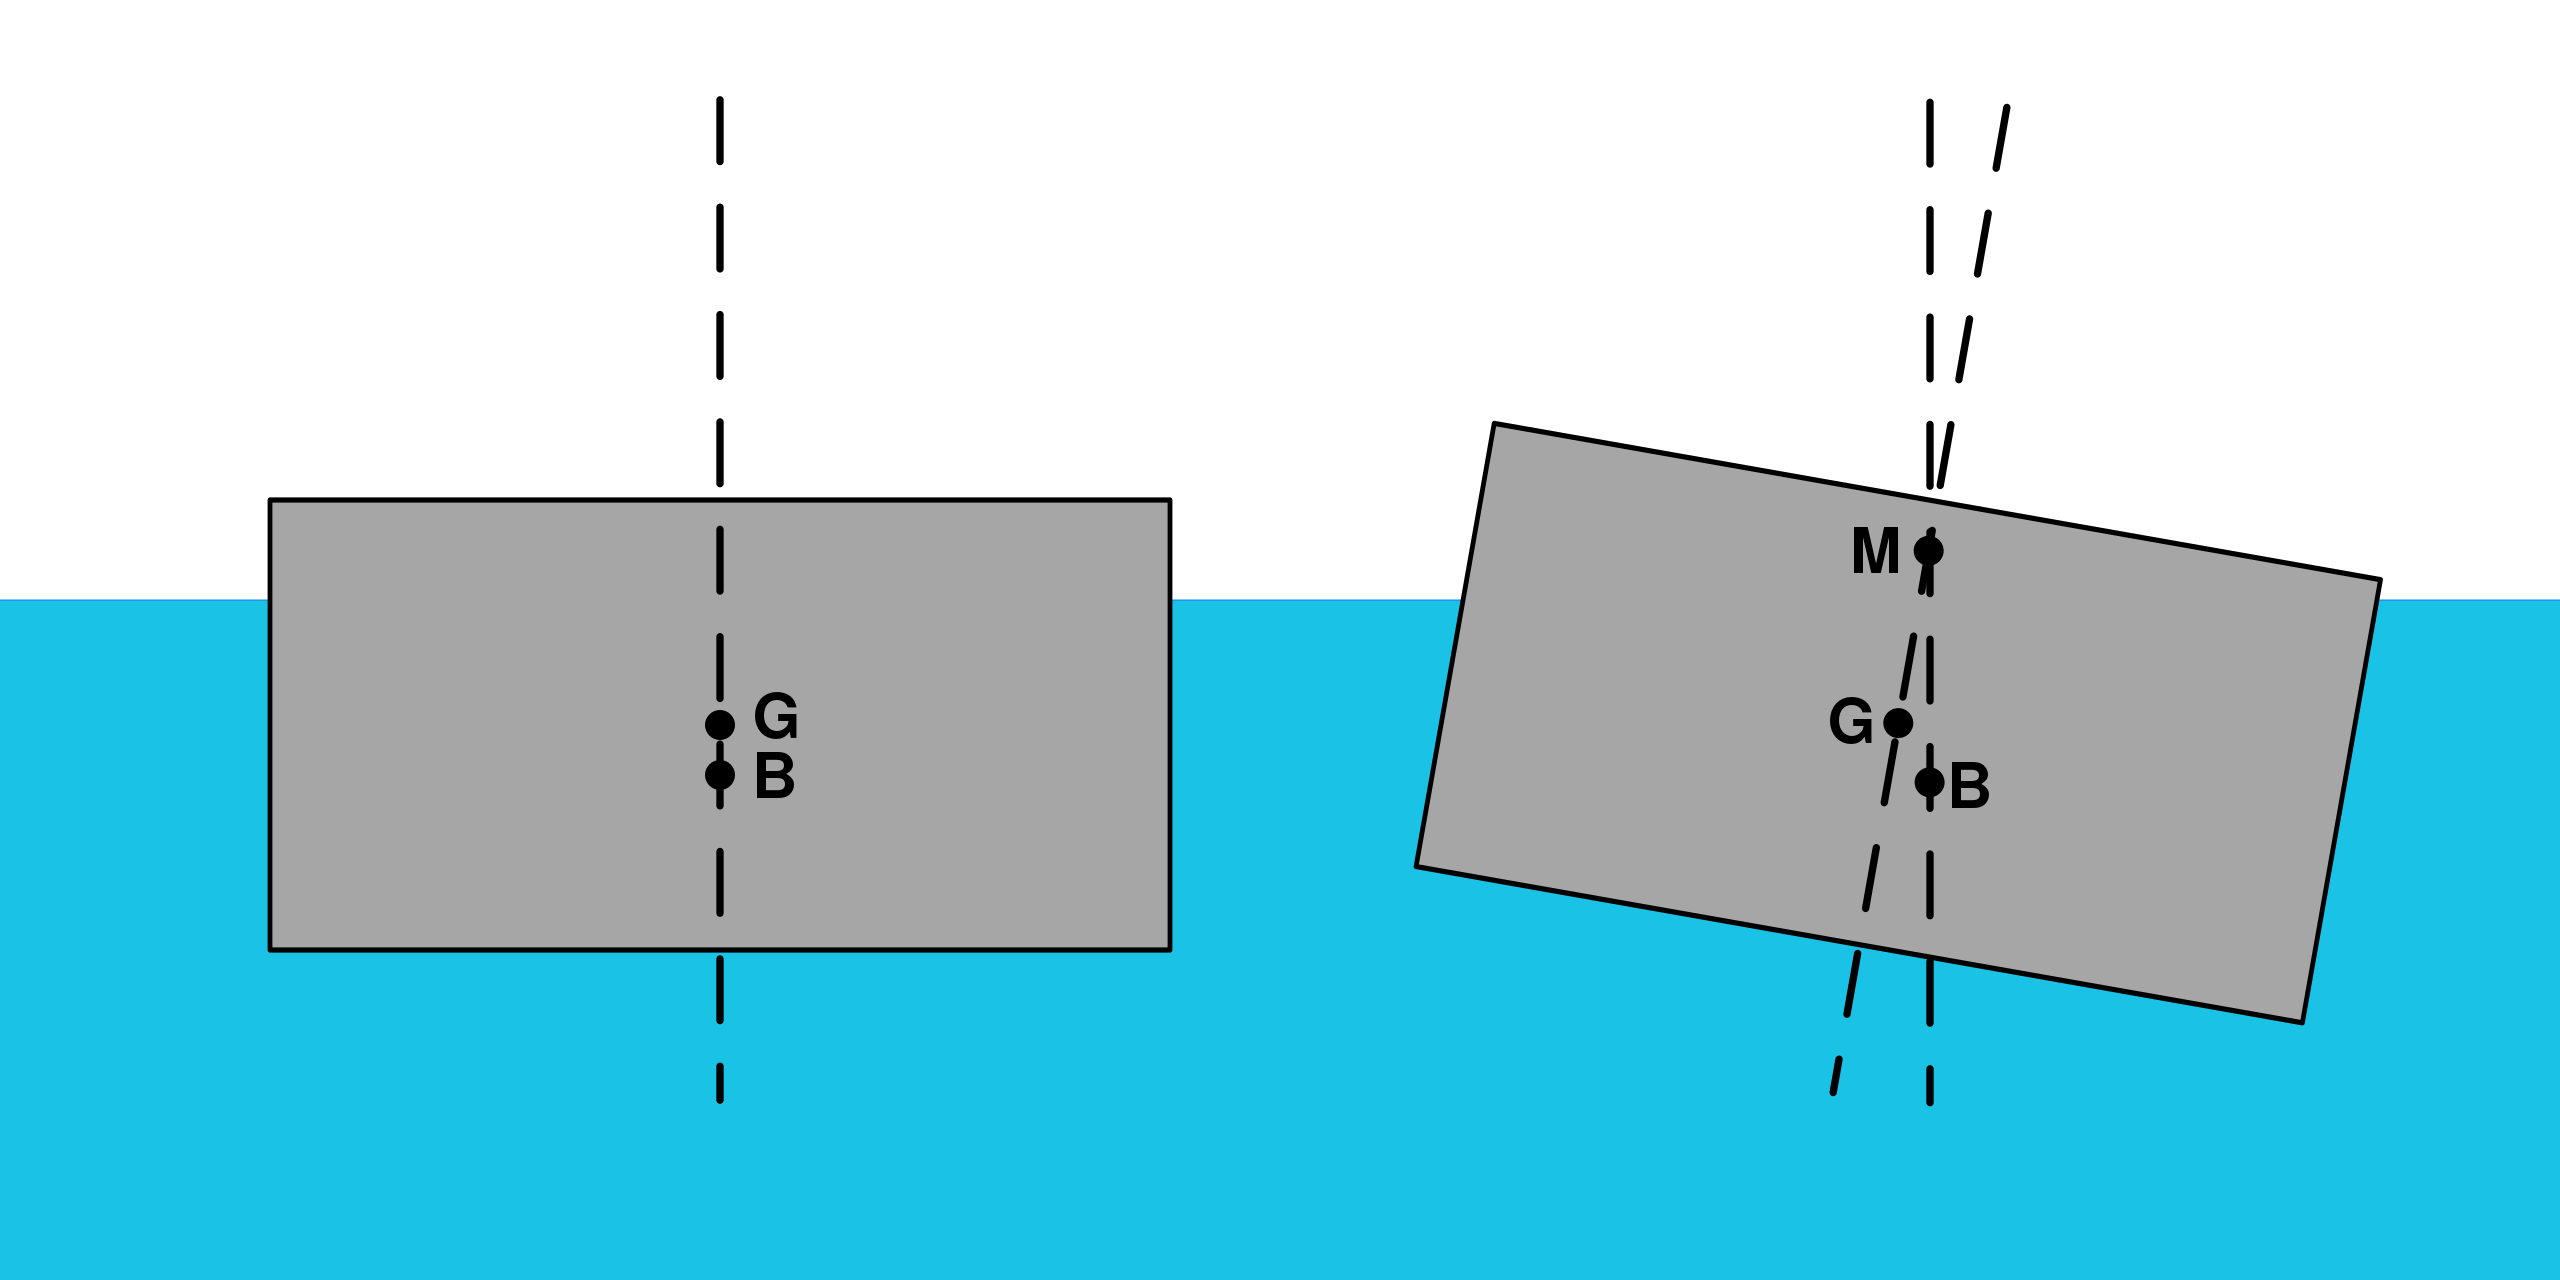
\includegraphics[width=0.5\linewidth]{Metacentriskhojd-svg.svg.png}
    \caption{Lage des Gewichtsschwerpunkt (G), Auftriebsschwerpunkt (B) und Metazentrum (M) bei aufrechtem, sowie gekrängtem Boot }
    \label{fig:enter-label}
\end{figure}
Zur Bewertung der Stabilität eines Schiffes müssen die folgenden drei Parameter bekannt sein: (i) die Anfangsstabilität (die sogeannte metazentrische Anfangshöhe), (ii) der Stabilitätsumfang und (iii) die Fläche unter der Hebelarmkurve. Die metazentrische Höhe ist der Parameter für den aufrichtenden Hebelarm. Mit dem Stabilitätsumfang wird die rechnerische Krängung des Schiffes in Winkelgraden bis zum Kenterpunkt bezeichnet und mit der Hebelarmkurve wird der jeweilige aufrichtende Hebelarm über den vollen Krängungsbereich bis zum Kenterpunkt des Bootes grafisch dargestellt. Der Hebelarm wächst bei zunehmender Krängung zunächst steil an, dann immer flacher an und wird bei noch stärkerer Krängung wieder geringer, bis er schließlich den Kenterpunkt (C) erreicht. Dieser liegt da, wo der Gewichtsschwerpunkt über den Auftriebsschwerpunkt hinauswandert. Mit der Fläche unter der Hebelarmkurve (A) lässt sich die Erfüllung der geplanten Mindeststabilität belegen.  https://de.wikipedia.org/wiki/Stabilit%C3%A4t_(Schiffsk%C3%B6rper))

\begin{figure}
    \centering
    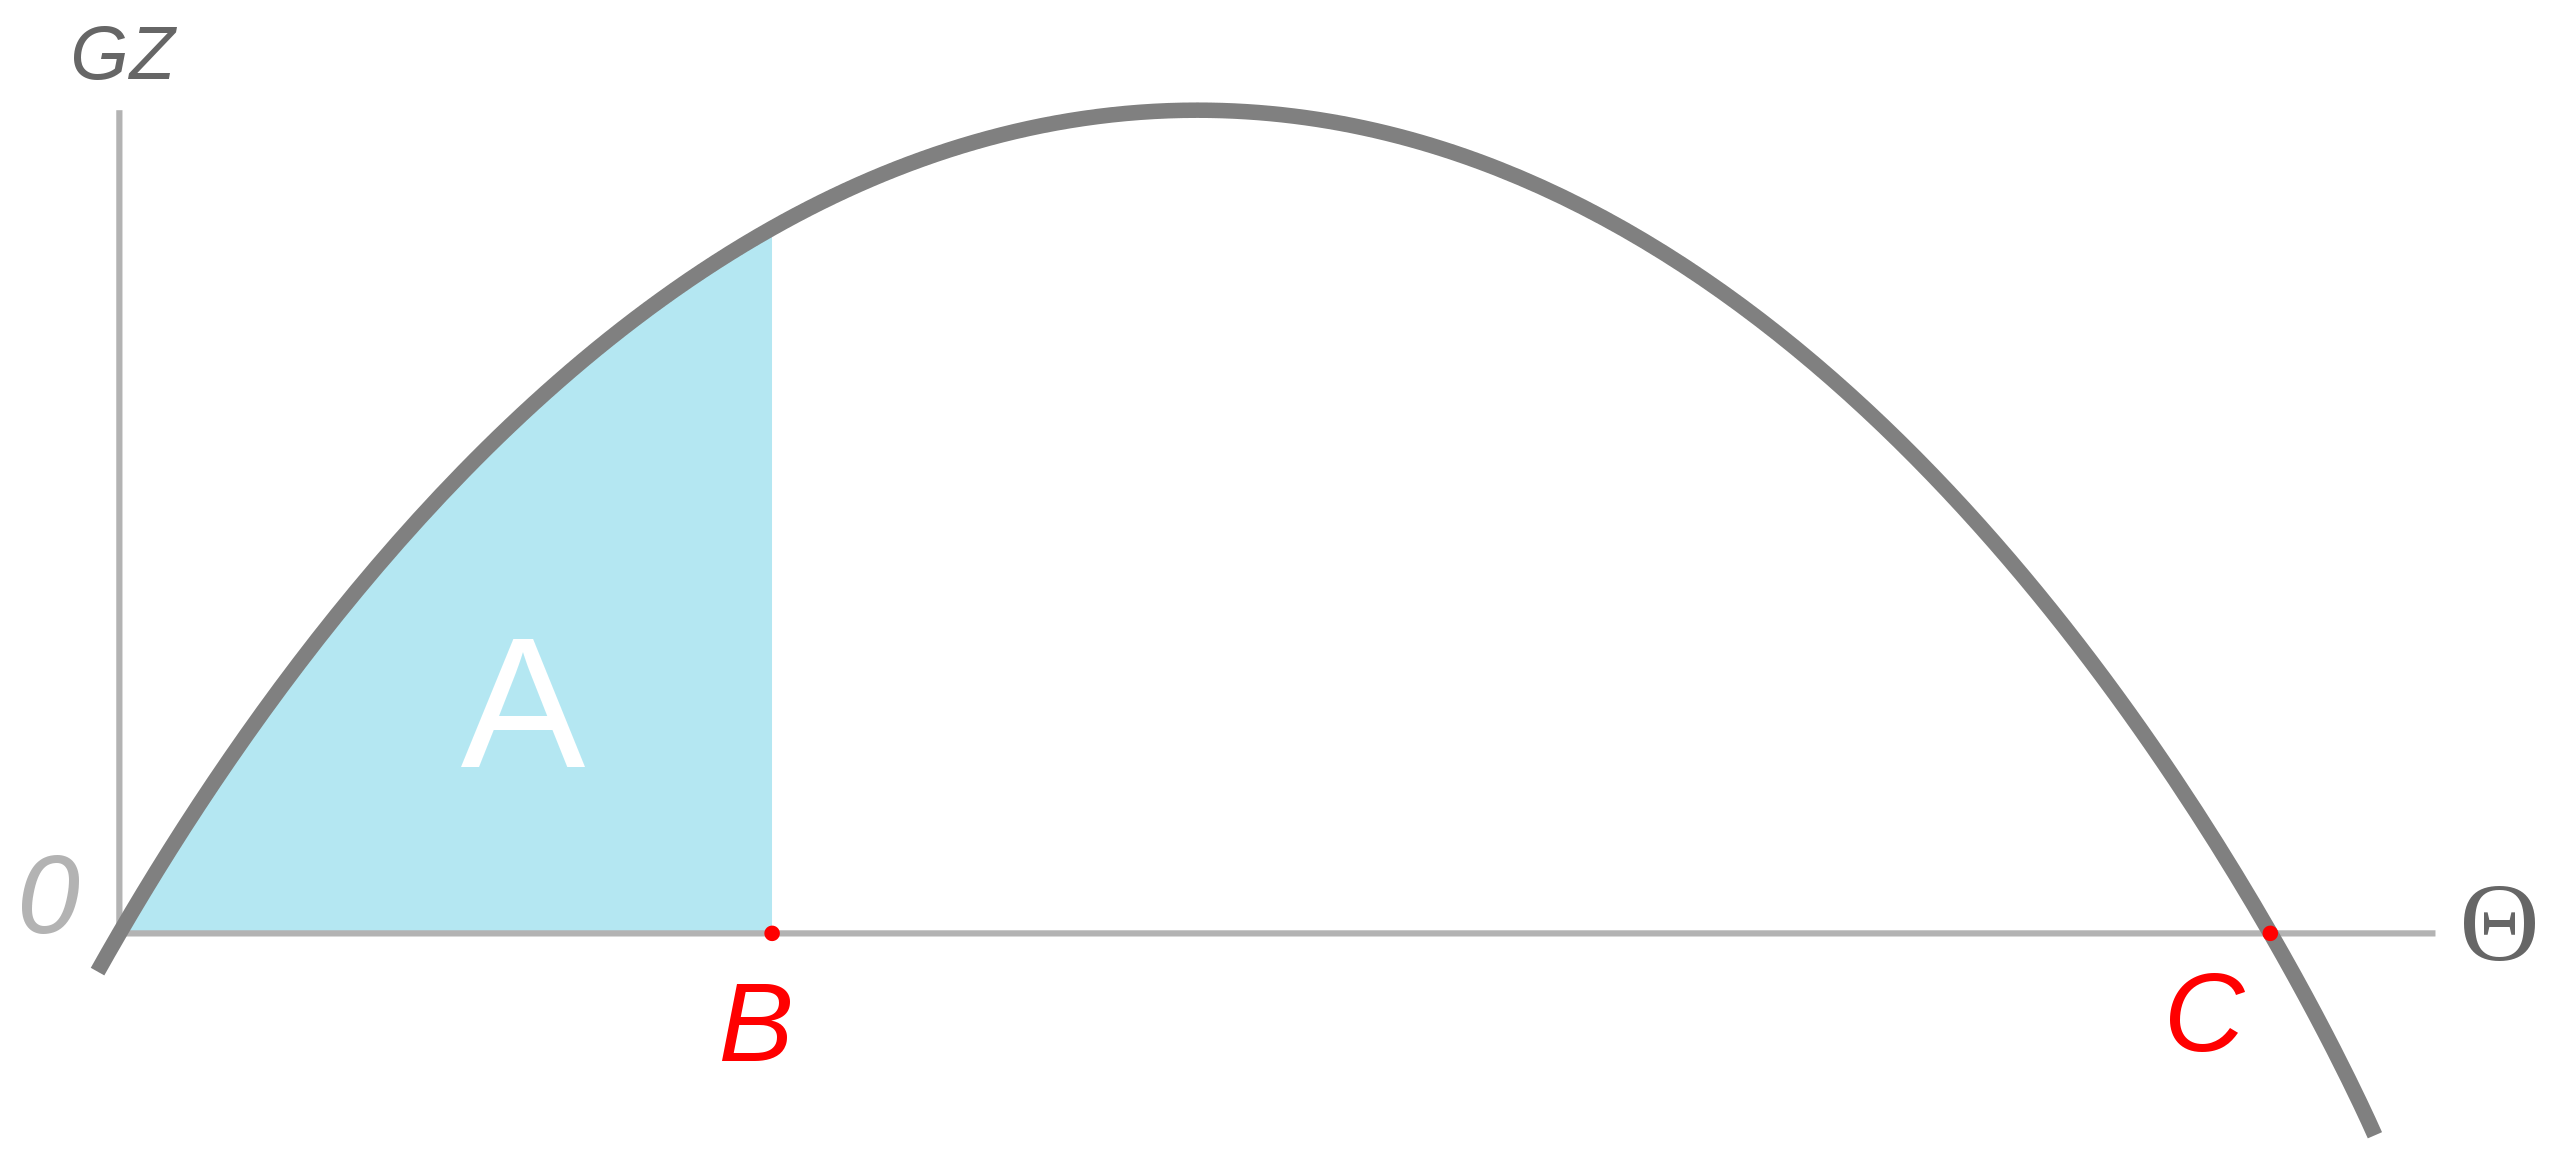
\includegraphics[width=0.5\linewidth]{Stability_curve_NT.svg.png}
    \caption{Hebelarmkurve}
    \label{fig:enter-label}
\end{figure}
Bei Segelbooten sind die Überlegungen zur Stabilität besonders wichtig, da sie mit ihren Segel für den Wind eine sehr grosse Angriffsfläche bieten. Ohne geeignete Gegenmassnahmen kippen sie schon bei geringen Windstärken um. Entscheidnd für die Stabilität eines Segelbootes sind dabei die Rumpfform und Gewichtsverteilung des Bootes. Die Krängung kann durch zwei Massnahmen wieder ausgeglichen und damit die Stabilität erhöht werden: 
\begin{itemize}
    \item Gewichtsstabilität – ein tief liegender Ballastkiel zwingt das Boot wieder in die aufrechte Lage (sogenanntes Stehaufmännchen-Prinzip).
    \item Formstabilität – die Form des Rumpfes begünstigt eine Rückkehr in die Ausgangslage.
\end{itemize}

\paragraph{Gewichtsstabilität}
Gewichtsstabilität durch Ballastkiel
Bei \href{https://de.wikipedia.org/wiki/Segelschiff}{Segelschiffen} wirkt ein \href{https://de.wikipedia.org/wiki/Kiel_(Schiffbau)}{Ballastkiel} als Gegengewicht der \href{https://de.wikipedia.org/wiki/Kr\%C3\%A4ngung}{Krängung} entgegen. Dieser enthält bis zu 50 \% der Masse des Schiffes und bewirkt so ein aufrichtendes Moment. Eine gewisse Krängung unter Segeln – je nach Bauart des Schiffes von 20 bis 45° – ist bei diesen Schiffen normal und stellt keine Gefahr für das Schiff dar. Im untenstehenden Bild ist G der \textit{\href{https://de.wikipedia.org/wiki/Gewichtsschwerpunkt}{Gewichtsschwerpunkt}} (Schwerpunkt des Bootes) und A der \textit{\href{https://de.wikipedia.org/wiki/Formschwerpunkt}{Formschwerpunkt}} (Schwerpunkt der verdrängten Wassermasse). Für mechanische Betrachtungen kann man sich die Gewichtskräfte als im Punkt G vereinigt denken und die Auftriebskräfte als im Punkt A. Mit zunehmender Krängung wandert der Gewichtsschwerpunkt weiter nach außen und es erhöht sich damit das aufrichtende \href{https://de.wikipedia.org/wiki/Drehmoment}{Drehmoment}. Manche Segelschiffe richten sich daher selbst bei einer Krängung von mehr als 120° noch selbstständig wieder auf\textsuperscript{\href{https://de.wikipedia.org/wiki/Stabilit\%C3\%A4t_(Schiffsk\%C3\%B6rper)\#cite_note-Seemannschaft,_Seite_163-1}{[1]}}. Erst durch sehr hohen \href{https://de.wikipedia.org/wiki/Seegang}{Wellengang} können sie mit dem Kiel nach oben gedreht werden und gelten daher als \href{https://de.wikipedia.org/wiki/Kentern}{kentersicher}. Dringen allerdings größere Mengen Wasser ins Bootsinnere, sinken sie wegen des hohen Ballastgewichts. Verliert ein solcher Rumpf, beispielsweise nach einer Grundberührung, seinen Ballastkiel, so ist kaum mehr Stabilität vorhanden und das Kentern faktisch nicht mehr zu verhindern. 
\begin{figure}
    \centering
    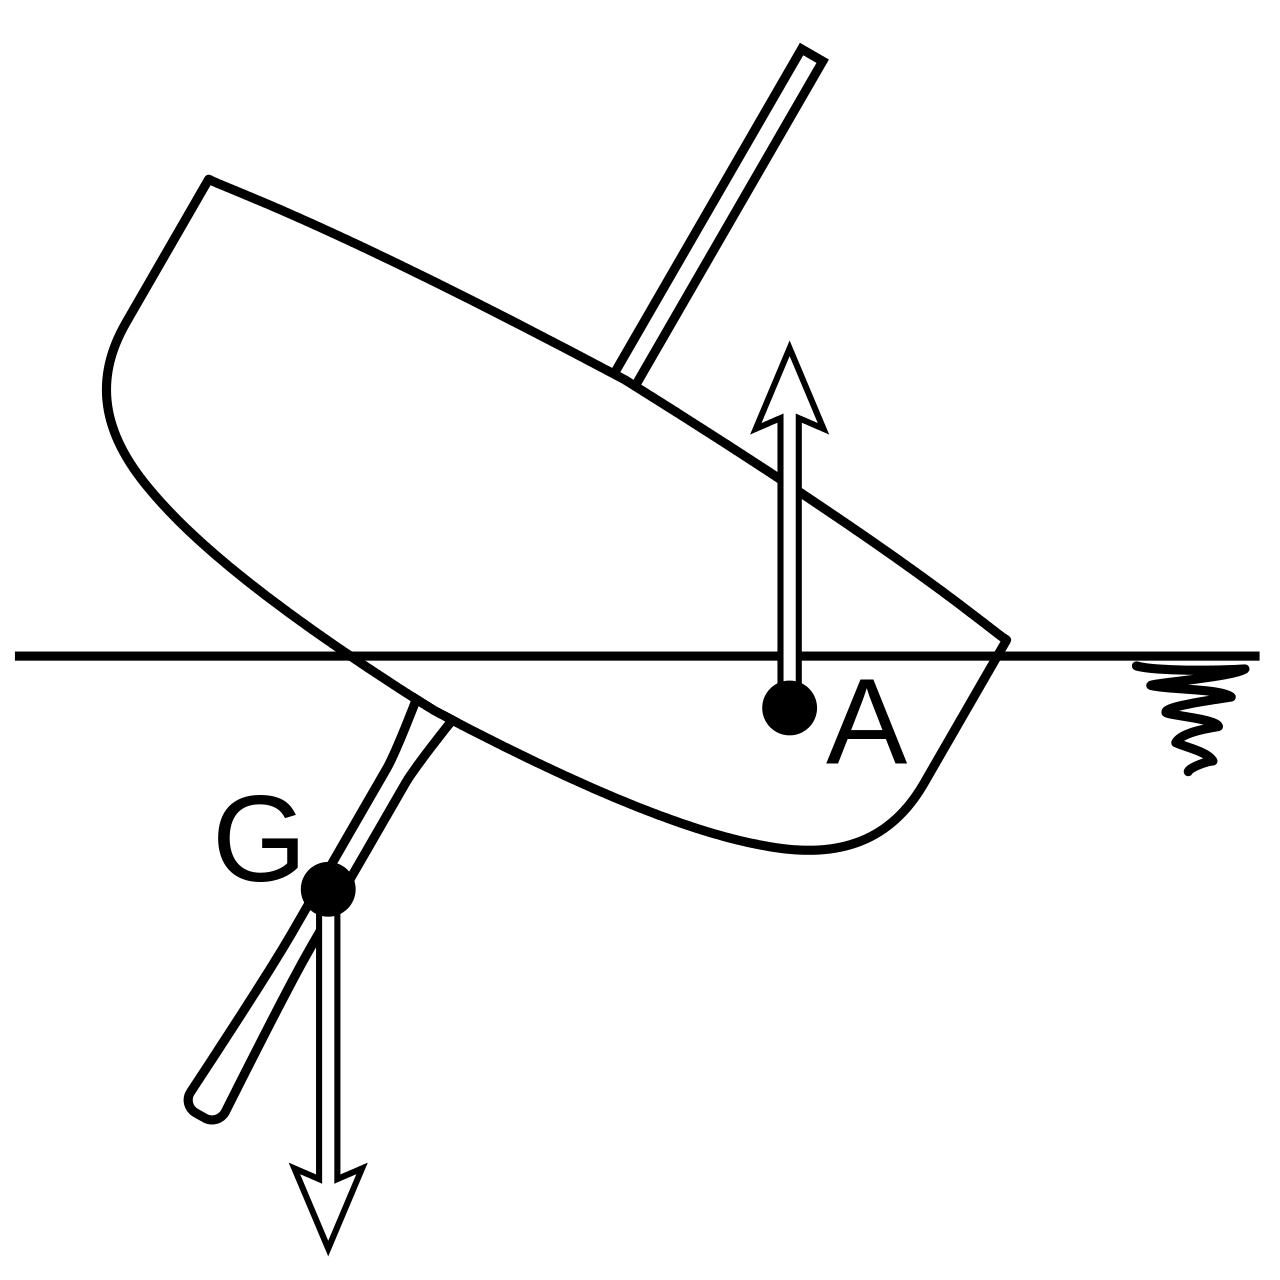
\includegraphics[width=0.5\linewidth]{Segeln_Gewichtsstabilitaet.svg.png}
    \caption{Gewichtsstabilität durch Ballastkiel }
    \label{fig:enter-label}
\end{figure}

\paragraph{Formstabilität}
Im Unterschied zu Kielyachten sind die meisten \href{https://de.wikipedia.org/wiki/Jolle}{Jollen} überwiegend formstabil. Das (meist ausklappbare) leichte Schwert einer Jolle hat keinen nennenswerten aufrichtenden Effekt. Auch \href{https://de.wikipedia.org/wiki/Segelkatamaran}{Katamarane} oder \href{https://de.wikipedia.org/wiki/Trimaran}{Trimarane} haben aufgrund ihrer Breite eine hohe Formstabilität. 
Im untenstehenden Bild ist G der Gewichtsschwerpunkt (Schwerpunkt des Bootes) und A der Formschwerpunkt (Schwerpunkt der verdrängten Wassermasse). In diesen Punkten kann man sich die Gewichts- bzw. Auftriebskräfte vereinigt denken. Für die Formstabilität ist die Lage von A ausschlaggebend. 

Bei aufrechter Lage des Bootes wird auf beiden Seiten des Rumpfes gleich viel Wasser verdrängt. A befindet sich dann mittig im Rumpfquerschnitt, es entsteht kein Drehmoment. Mit zunehmender Krängung (siehe Bild) wird Wasser vor allem auf einer Seite des Rumpfes verdrängt. Dadurch wandert A nach außen, es entsteht ein Drehmoment. Je breiter das Boot ist, desto weiter wandert A nach außen und desto stärker ist das aufrichtende Drehmoment. Wenn die Krängung zu groß wird, nimmt das Drehmoment allerdings wieder ab, weil dann der breite Rumpf gekippt ist und A wieder näher zur Mitte liegt. Eine leichte Krängung wird daher durch das kräftige aufrichtende Drehmoment kompensiert („Wasserwiderstand“), während eine zu starke Krängung zum Kentern des Bootes führt. Katamarane kentern, wenn die Krängung 90° erreicht.\textsuperscript{\href{https://de.wikipedia.org/wiki/Stabilit\%C3\%A4t_(Schiffsk\%C3\%B6rper)\#cite_note-Seemannschaft,_Seite_163-1}{[1]}} 

Es gibt sogar Beispiele für komplett formstabile Bootstypen mit negativer Anfangsstabilität. Diese haben im Ruhezustand keine aufrechte Schwimmlage. 
\begin{figure}
    \centering
    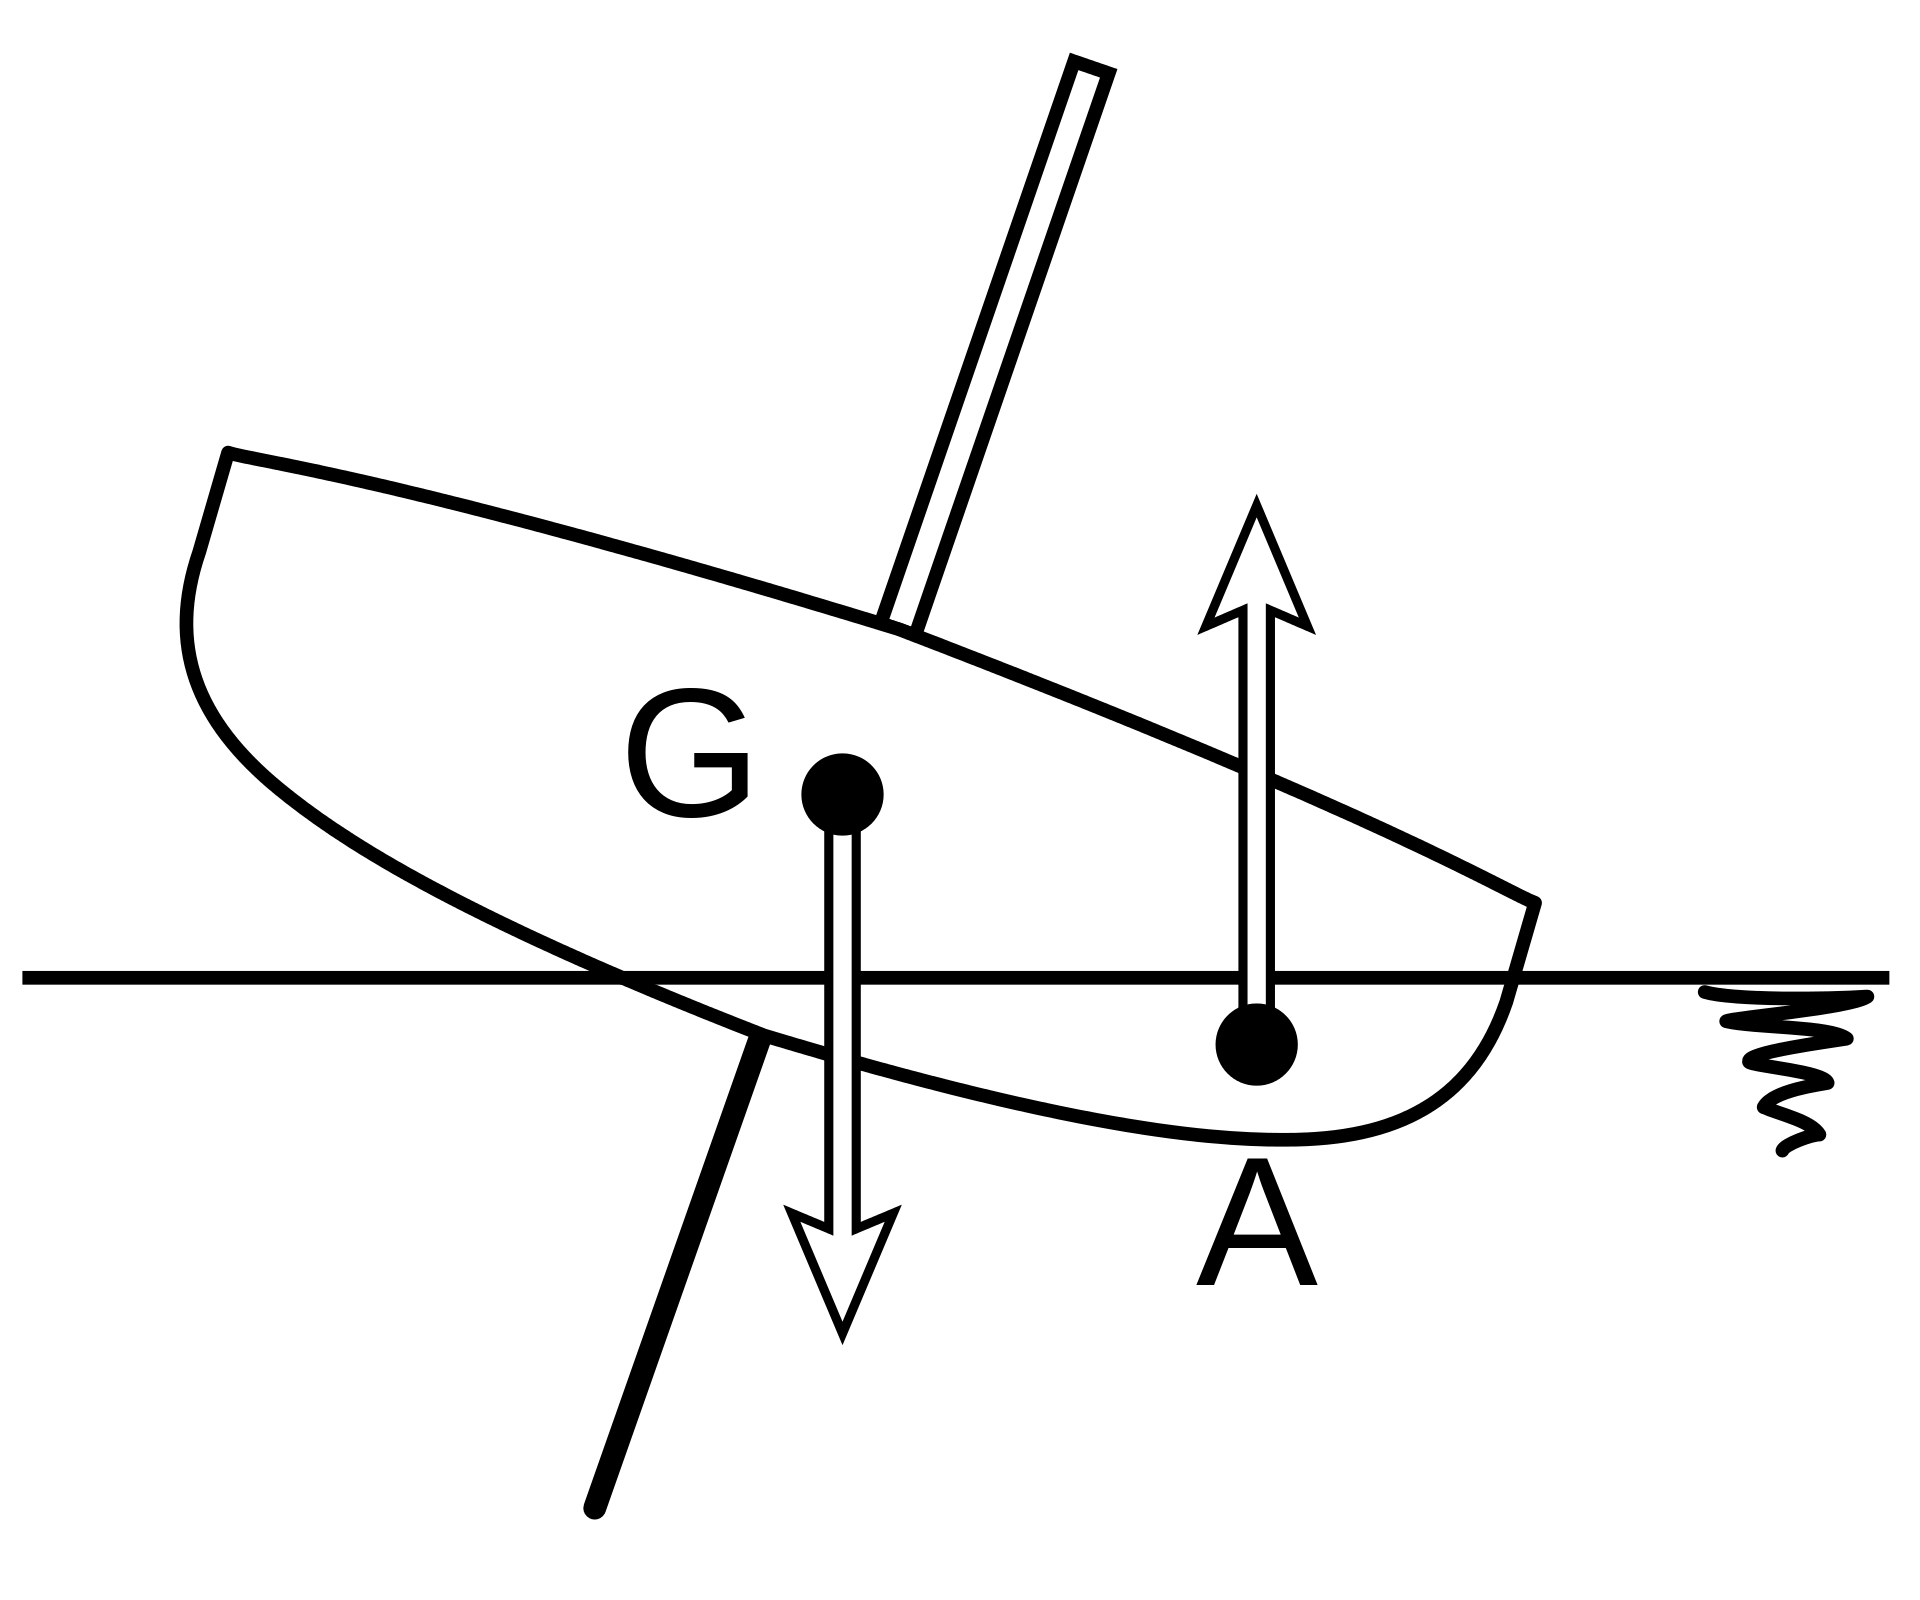
\includegraphics[width=0.5\linewidth]{Segeln_Formstabilitaet.svg.png}
    \caption{Formstabilität }
    \label{fig:enter-label}
\end{figure}

\paragraph{Gegenmaßnahmen bei großer Krängung}

Ein Segler hängt im Trapez, um den Katamaran auszubalancieren.Sowohl bei Kielbooten als auch bei Katamaranen oder Jollen kann die Krängung reduziert werden, indem sich die Crew „auf die hohe Kante setzt“, das heißt sich im \href{https://de.wikipedia.org/wiki/Luv_und_Lee}{Luv} an die Reling setzt, oder die Segelfläche reduziert wird (\href{https://de.wikipedia.org/wiki/Reffen}{Reffen}). Bei sportlich gesegelten \href{https://de.wikipedia.org/wiki/Jolle}{Jollen} hängt sich die Crew in ein \href{https://de.wikipedia.org/wiki/Trapez_(Segeln)}{Trapez}, um weiter nach Luv ausreiten zu können.\textsuperscript{\href{https://de.wikipedia.org/wiki/Stabilit\%C3\%A4t_(Schiffsk\%C3\%B6rper)\#cite_note-2}{[2]}} Beim sportlichen Segeln von Jollen kann eine Kenterung schon mal vorkommen. Sie sind im Gegenzug mit Schwimmkörpern ausgerüstet, so dass sie trotz Kenterung nicht sinken. Jollen sind dennoch nicht für die Hochsee geeignet und selbst gute Jollensegler werden bei angekündigten \href{https://de.wikipedia.org/wiki/Beaufort-Skala}{Windstärken} von mehr als 6 nicht mehr ablegen. 

Durch die Krängung wird automatisch die wirksame Segelfläche reduziert, auch die Form des Rumpfes bevorzugt einen bestimmten Krängungswinkel, bei dem das Schiff die höchste Geschwindigkeit erreichen kann. Daher wird durch starke Krängung das Schiff langsamer, zudem wird der Aufenthalt an Bord ungemütlicher. Auch steigt die Gefahr, dass es durch zu starke Krängung zu einem sogenannten \href{https://de.wikipedia.org/wiki/Sonnenschuss}{Sonnenschuss} kommt und das Schiff „aus dem Ruder läuft“\textsuperscript{\href{https://de.wikipedia.org/wiki/Stabilit\%C3\%A4t_(Schiffsk\%C3\%B6rper)\#cite_note-3}{[3]}} und „in den Wind schießt“.\textsuperscript{\href{https://de.wikipedia.org/wiki/Stabilit\%C3\%A4t_(Schiffsk\%C3\%B6rper)\#cite_note-4}{[4]}} Noch schlimmer ist es, wenn die Nock des \href{https://de.wikipedia.org/wiki/Baum_(Segeln)}{Großbaums} ins Wasser eintaucht, was zu schweren Schäden am \href{https://de.wikipedia.org/wiki/Takelage}{Rigg} führen kann. Daher kann durch rechtzeitiges Reffen – trotz verkleinerter Segelfläche – die Geschwindigkeit zunehmen. 

 


Der Entwicklungsprozess des Kiels ist aufgrund der kaum vorhandenen Literatur zu dieser Frage sehr aufwendig. [???KANNST DU DIESE AUFFÜHREN????]\\ 

Die erste Fragestellung in diesem Bereich, ist ob ein Kiel oder ein Schwert verwendet werden soll. Der Unterschied zwischen Kiel und Schwert besteht darin, dass ein Kiel über ein beträchtliches Eigengewicht verfügt, das in der Regel durch die Verwendung von Balast  erreicht wird, während  ein Schwert lediglich den Wasserwiederstand nutzt und in der Regel aufholbar ist. Kiele werden hauptsächlich bei Jachten verwendet; Schwerter bei Jollen. 

 um das Boot aufrecht zu halten
Aufrichtendes Moment


Ein Kiel ist ein Teil des Rumpfes eines Bootes, der dafür sorgt, dass das Boot aufrecht bleibt und sich nicht auf die Seite legt. Er ist normalerweise das tiefste Teil des Bootes und erstreckt sich vom Bug bis zum Heck. Der Kiel ist sehr wichtig, um das Boot stabil zu halten und es steuerbar zu machen 

Neben der tragenden Funktion hat der Kiel bei Wasserfahrzeugen auch eine hydrodynamische Funktion. Er vergrößert den \href{http://en.wikipedia.org/wiki/de:Lateralplan}{Lateralplan} des Schiffes und erhöht damit seinen Querwiderstand im Wasser, verringert also die Abdrift durch Seitenwind. Dies ist für \href{https://www.modellbau-wiki.de/wiki/Segel}{Segelschiffe} besonders wichtig, um am Wind oder gegen den Wind (sogenanntes Kreuzen) zu segeln. Bei \href{https://www.modellbau-wiki.de/wiki/Segel}{Segelbooten} und kleinen Segelschiffen (z.B. \href{http://en.wikipedia.org/wiki/de:Ewer}{Ewer}) wird diese Funktion des Kiels durch \href{https://www.modellbau-wiki.de/wiki/Schwert_(Schiffbau)}{Schwerter} ergänzt, die in der Mitte des Kiels (Zentralschwert) oder seitlich des Rumpfes (Seitenschwert) angebracht sein können. Zudem ist der \textbf{Kiel} für die Gewichtsstabilität des Schiffes verantwortlich, verringert somit die \textit{Krängung} (Schräglage) und verhindert ein Kentern des Schiffes.  

Ein Kiel ist bei den meisten Wasserfahrzeugen zu finden, egal ob sie durch Wind oder Motor angetrieben werden. Es wird allgemein als eine feststehende Unterwasserverlängerung verstanden, die aus dem Boden eines Bootes herausragt, obwohl einige Versionen beweglich sind. Diese Verlängerung bietet Stabilität und widersteht seitlichen Bewegungen oder Drift. Seitwärtsbewegungen werden durch Wind oder Querströmungen verursacht und werden nicht nur durch Form und Tiefgang (Tiefe) einer Kielkonstruktion, sondern auch durch ihr Gewicht (oder Ballast) entgegengewirkt. 

Ein Schwert ist eine parallel zur Fahrtrichtung angebrachte senkrechte Platten und dient zur Verminderung der Abdrift beziehungsweise zur Umsetzung der Abdrift in Vortrieb. 
\\
Für dieses Boot wurde sich für ein Kiel entschieden, da es auf dem Boot keine möglichkeit gibt, Gewicht zu verschieben. Bei Jollen ist in der regel ein Segler auf dem Boot, welcher sehr viel mit seinem eigenen Körpergewicht steuert. Bei den meisten Jachten spielt das Körpergewicht der Segler keine oder nur eine untergeordnete Rolle.





\section{Entscheid für ein Kielboot}
Jollen, bzw. Schwertboote werden vorallem mit dem Eigengewicht des Seglers gesegelt. Seine Positiotion und seine Bewegungen Spigelen sich direkt in der Segelleistung wieder. Kentern gehört zum alltag von Jollnseglern genauso wie das Nasswerden.

Kielboote, bzw Yachten sind da etwas anders.Die Position der Mannschaft spielt keine bedeutende Rolle. Kielboote Kentern unter normalen Bedingungen nicht. Da ein Autonomes Segelboot über keine sich Bewegende Manschaft verfügt, noch irgendwelche Möglichkeiten zur verschiebung von Gewichten hat, ist ein Kielboot viel die einfachere Lösung.



\subsection{






%->	Baupläne werden generiert als Resultat



\section{Materialauswahl und -begründung }
% Turn around 

Die strukturell tragenden Elemente sind Hauptsächlich aus Holz gebaut. Dies hat den entscheidenden Vorteil der einfachen Verarbeitung. Ebenso hat Holz den Vorteil, dass es an sich schon schwimmt da es weniger Dicht als Wasser ist. Konkret werden zwei Holzarten verwedet. Zum einen Tannenholz und zum anderen Balasaholz. Das Tannenleimholz wird mit einer Stärke von 18mm verbaut und ist das kostengünstigste Holz was in dieser Kategorie im Baumarkt zu finden ist.
Alternativen zu Holz wären diverse Kunststoffe wie PLA, ABS, PETG, ect. welches durch 3D Druck geformt werden können. Jedoch wären die Kosten bei dieser Methode deutlich höher und eine gleiche Stabilität wie bei Holz zu erreichen wäre eine Herausforderung.
Ebenfalls möglich sind Rippenelemente aus Metallen, wie zum Beispiel Aluminium. Die Materialkosten sind bei Metallen jedoch weitaus höher und die Bearbeitung um ein vielfaches Komplizierter weshalb sich dagegen entschieden wurde.
\\
Fu¨ r die Beplankung wird Balsaholz verwendet, da dieses sehr weich, biegsam und einfach zu be- und verarbeiten ist. Es ist im Modellbau weit verbreietet und in diversen Stärken verfügbar. In geringen Stärken von 1mm laässt es sich gut an die Form des Bootes anpassen.
% Balsaholz ABschnitt hinzufügen

\subsection{Fiberglas}
Da Balsaholz sehr porös ist, darf es unbehandelt nicht Wasser ausgesetzt werden. Selbst wenn es mit Lack gegen Feuchtigkeit geschützt wird, ist eine Balsaholzuhülle zu wenig robust, um die Aussenhülle des Bootes zu bilden.

Für die äussere Hülle werden Fiberglasmatten verwendet. Diese sorgen für eine stabile Hülle und schützen das Boot zusätzlich vor seitlichen Zusammenstössen. Ebenfalls sorgen sie dafür, dass das Boot dicht ist und kein Wasser hineinfliesst. Alternativ hätte man das Boot lediglich mit Epoxidharz abdichten können. Dies hätte aber dazu geführt, dass das Boot um ein vielfaches weniger stabil wäre. 

\section{Prozess der Konstruktion}
Bei der Konstruktion geht es um die Erstellung von Plänen. Das erfolgt bei komplexeren Konstruktionen immer computergestützt mittels sogenannten \ac{cad} Programmen. 

\subsection{Applikation}
Computer Aided Design (CAD) ist eine Form des technischen Zeichens, welches einem ermöglicht Modelle in Drei dimensionalen Raum zu gestalten. Somit lässt ist es verhältnissmässig einfach Technische Zeichnungen anzufertigen. Es gilt als eines der Wichtigsten Werkzeuge zur Planung von Maschienen und Geräten da sie so einfacher Vorstellbar sind und der Materialbedarf geplant werden kann. Die Konstruktion dieses Projekt beginnt mit dem erlernen von den Programmen Autodesk Inventor und Autodesk Fusion 360. 
Beide Programme verfolgen einen ähnlichen Ansatz und sind ähnlich Aufgebaut. Im Vergleich zu Inventor ist Fusion deutlich nutzerfreundlicher und ermöglicht es Projekte über eine Cloud einfacher zu speichern und von Unterwegs zu Bearbeiten. Die Programme von Autodesk wurden gewählt, da diese für den Persönlichen oder Bildungsgebrauch kostenlos sind. Open Source Programme wie FreeCAD wurden nicht gewählt, da diese weniger Intuitiv zum lernen sind und meist über weniger Funktionen verfügen. Programme welche als deutlich Leistungsstarker gelten wie NX Siemens oder Solidworks sind aufgrund der Lizensierungskosten für dieses Projekt nicht in Frage gekommen. 

\subsection{Konstruktionsvorgang des Rumpfes}
Da eine ebene Fläche für die Positionierung der Solarpanels benötigt wird, wird das Deck flach ausgelegt. Es bildet den Ausgangspunkt des Entwurfs. In einer Skizze wird die spätere Bootsform mithilfe gezeichnet. Da das Boot Wellen und Wetterbeständig sein sollte, muss das Boot über genügend Auftrieb verfügen. Daher wird eine Länge von 2.2m gewählt. \\
Für die maximale Breite werden 0.55m verwendet. Dies entspricht einem Viertel der Länge. Das Verhältnis zwischen der Länge und der Breite ist der Einflussreichste Faktor welcher über  Stabilität und die Manövrierfähigkeit. Ein Verhältnismässig Breites Boot ist deutlich stabiler als ein schmaleres, jedoch weniger Manövrierfähig. \cite{Seemannschaft} \\
\begin{figure}[H]
    \centering
    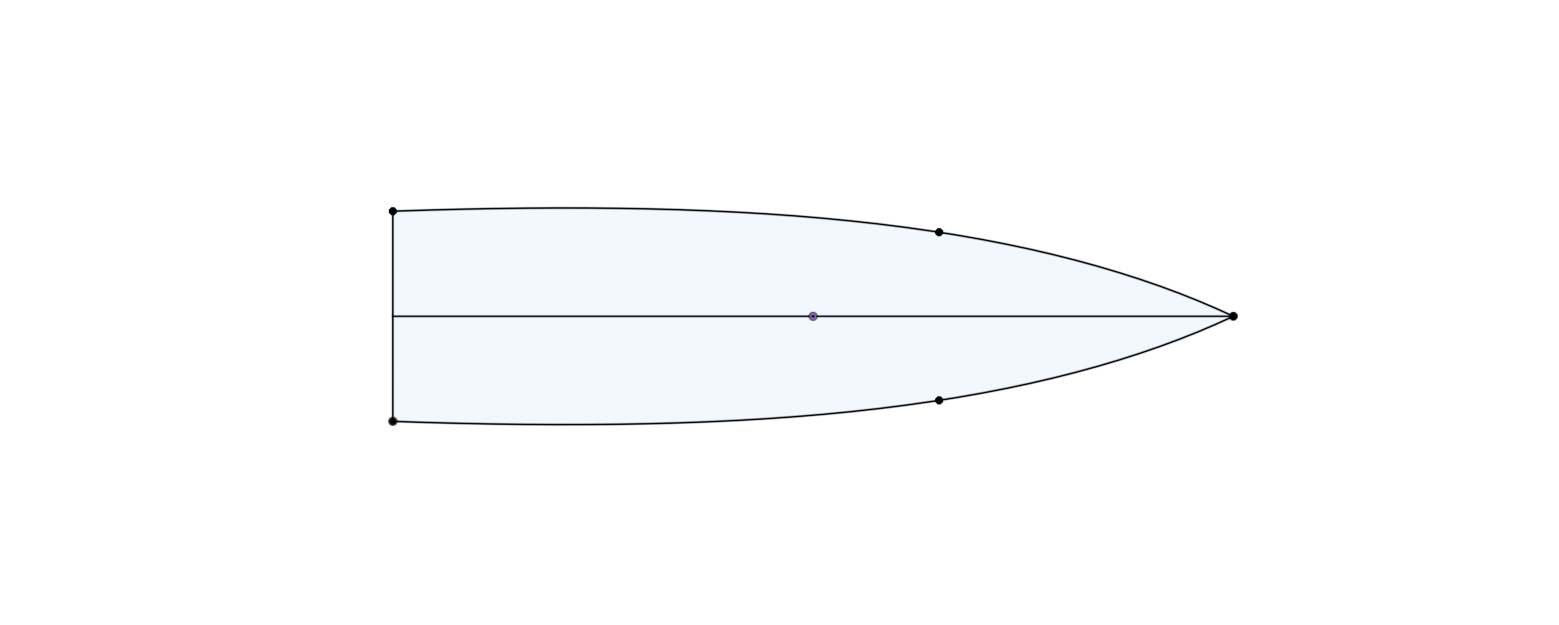
\includegraphics[width=1\linewidth]{assets/boot sketch top.png}
    \caption{Topansicht des Boots}
   
\end{figure}
In einem nächsten Schritt wird die Seitenansicht des Bootes konstruiert. Dieses Boot verfügt über einen angewinkelten Vorsteven und ein flaches Heck. Das Flache Heck wird gewählt, da die Befestigung des Ruders so am einfachsten ist und der Bug nach Hinten angewinkelt.

\begin{figure}[H]
    \centering
    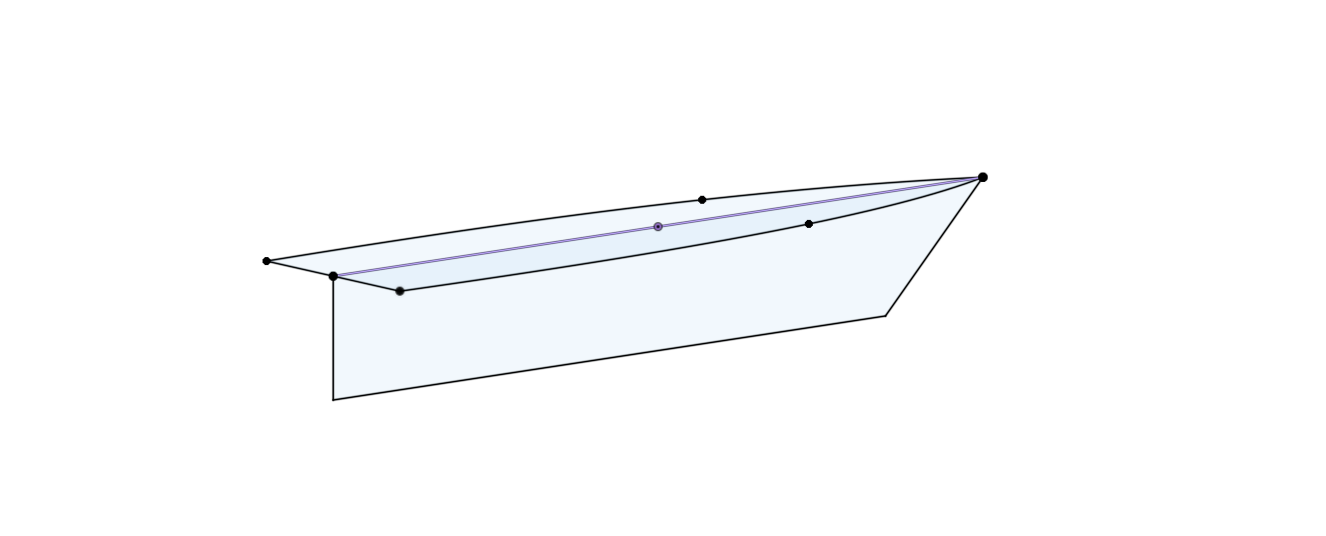
\includegraphics[width=1\linewidth]{assets/boot_skizze_2.png}
    \caption{Seitenansicht mit Steven}
    
\end{figure}

Als Heckform wurde eine leicht eingebeulte Form verwendet, welche dem Boot verhilft, senkrecht im Wasser zu stehen.

\begin{figure}[H]
    \centering
    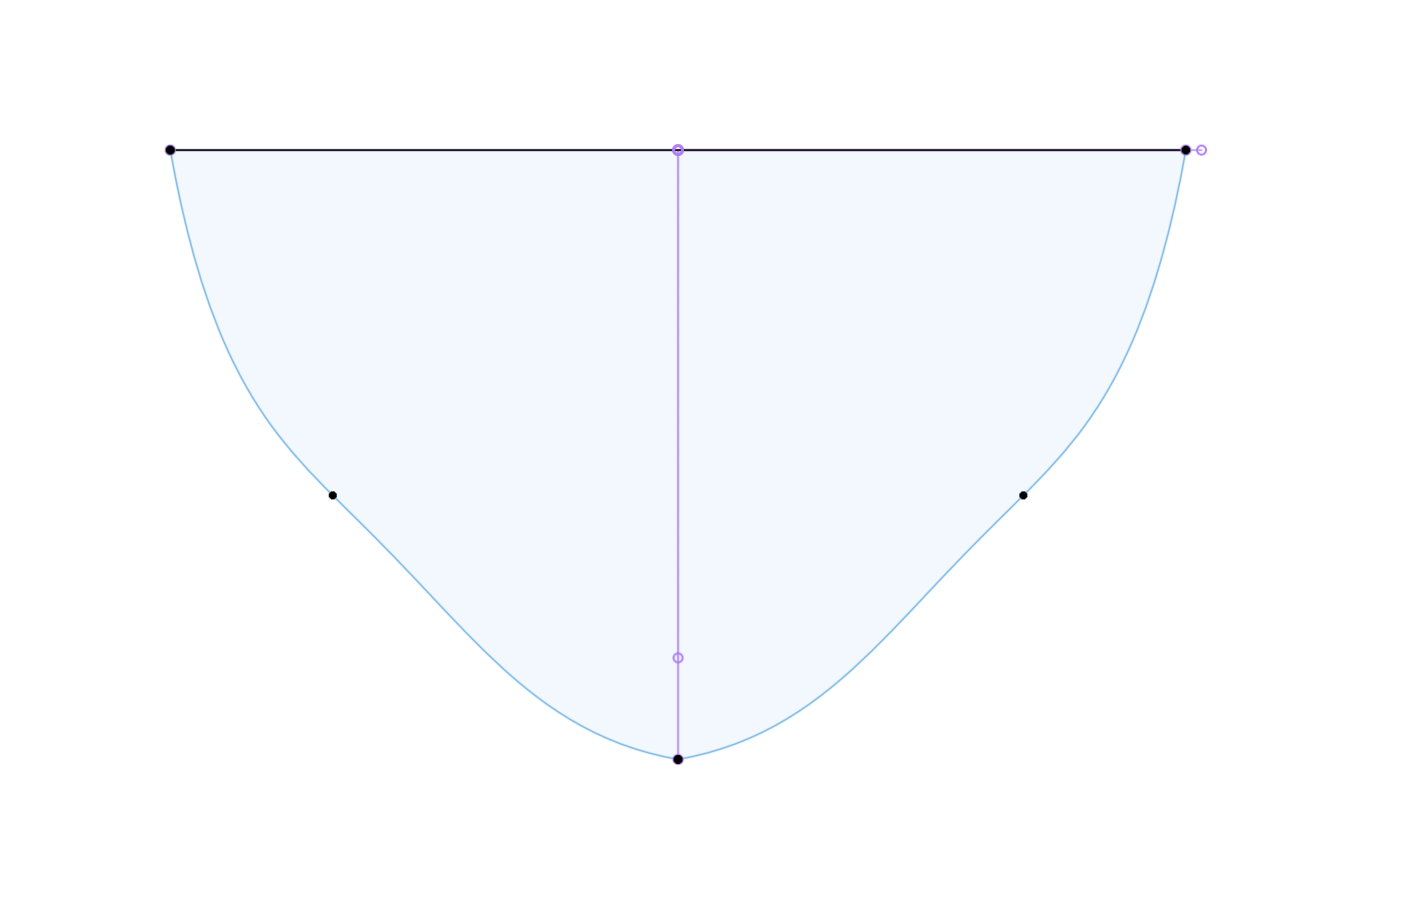
\includegraphics[width=0.6\linewidth]{assets/Heck_boot.png}
    \caption{Heckansicht}
   
\end{figure}

Mit dem Erhebungswerkzeug (Loft Tool) wird im Anschluss aus den Skizzen ein Körper berechnet. Unten am Rumpf wird zudem eine Begradigung hinzugefügt welche es ermöglicht den Kiel senkrecht am Boot zu montieren.
\begin{figure}[H]
    \centering
    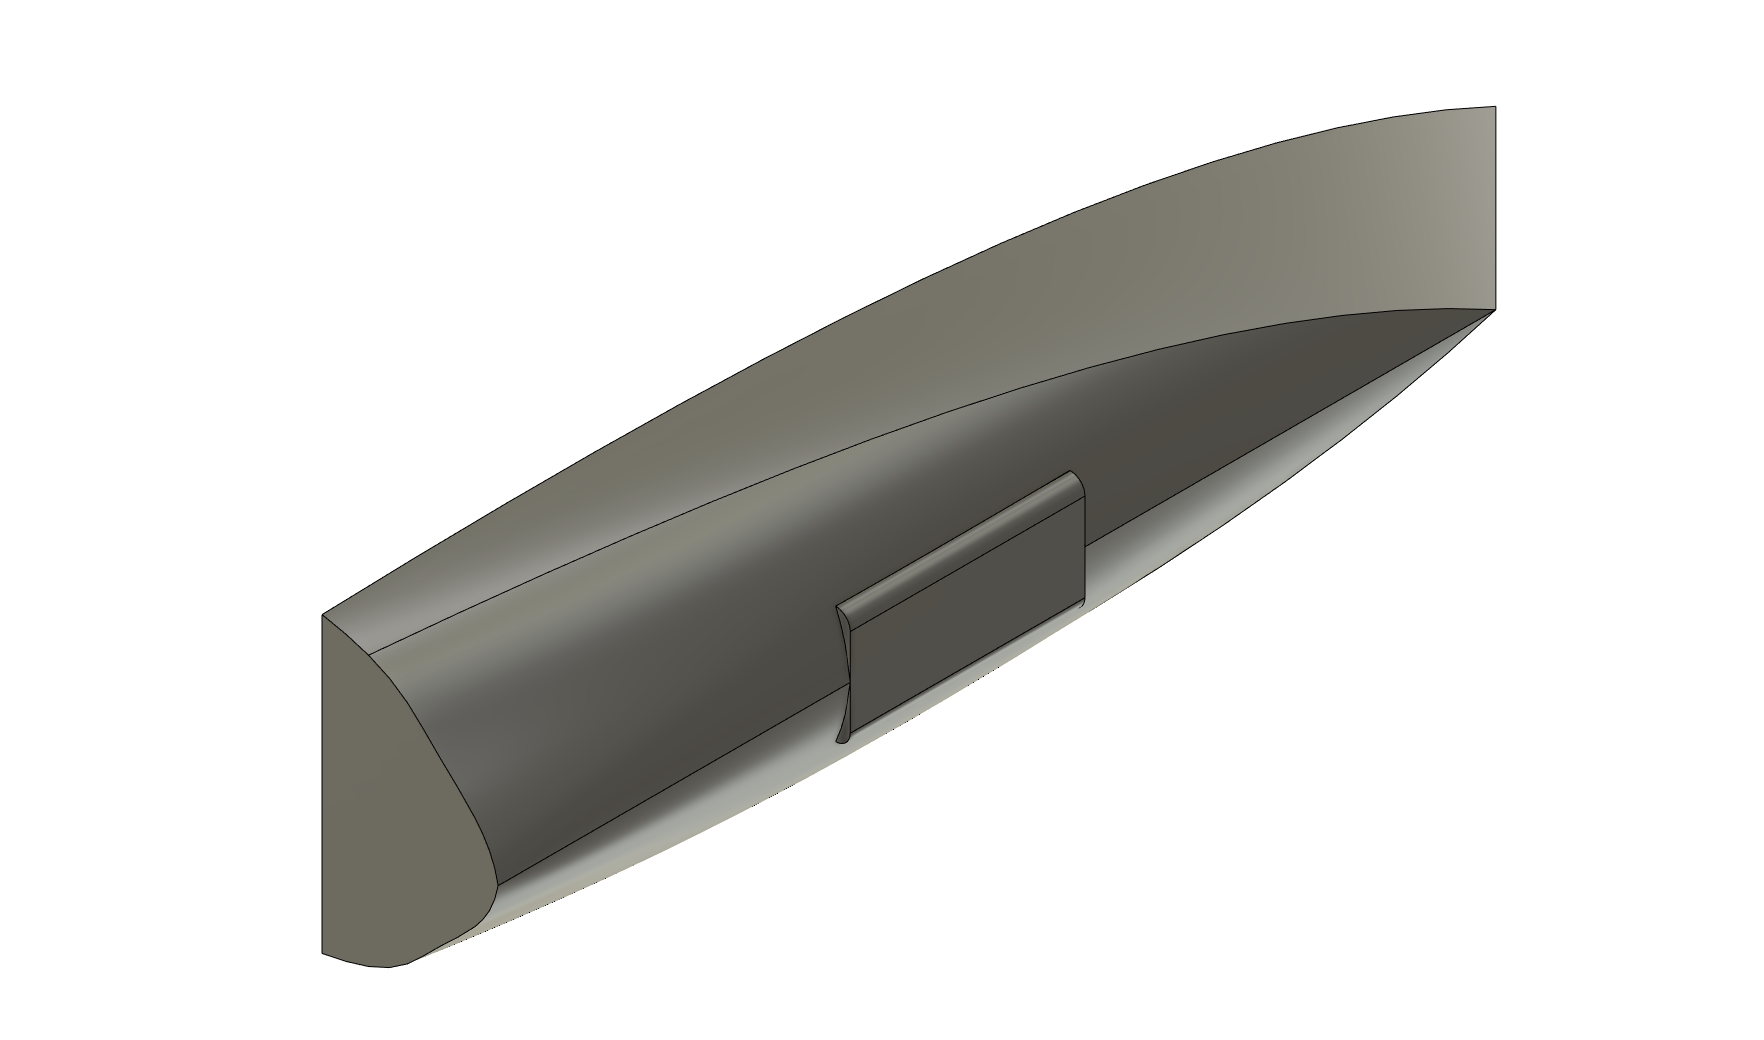
\includegraphics[width=0.75\linewidth]{assets/kielbefestigung2image.png}
    \caption{Fläche zur Montierung es Kiels}
    \label{fig:enter-label}
\end{figure}

Im Anschluss wird die Form mit einer Randstärke von 4 cm innen ausgehölt. 
\begin{figure}[H]
    \centering
    \includegraphics[width=1\linewidth]{assets/Hohlkörper.png}
    \caption{Schnittbild Hohlkörper}

\end{figure}
Im nächsten Schritt wird der bereits ausgehöhlte Körper auf zwölf Spanten mit einem einheitlichem Abstand 14 cm reduziert. Die Spanten haben eine Stärke von 18 mm. Die Masse der Spanten verjüngen sich von der Mitte zum Bug und Heck hin.

\begin{figure}[H]
    \centering
    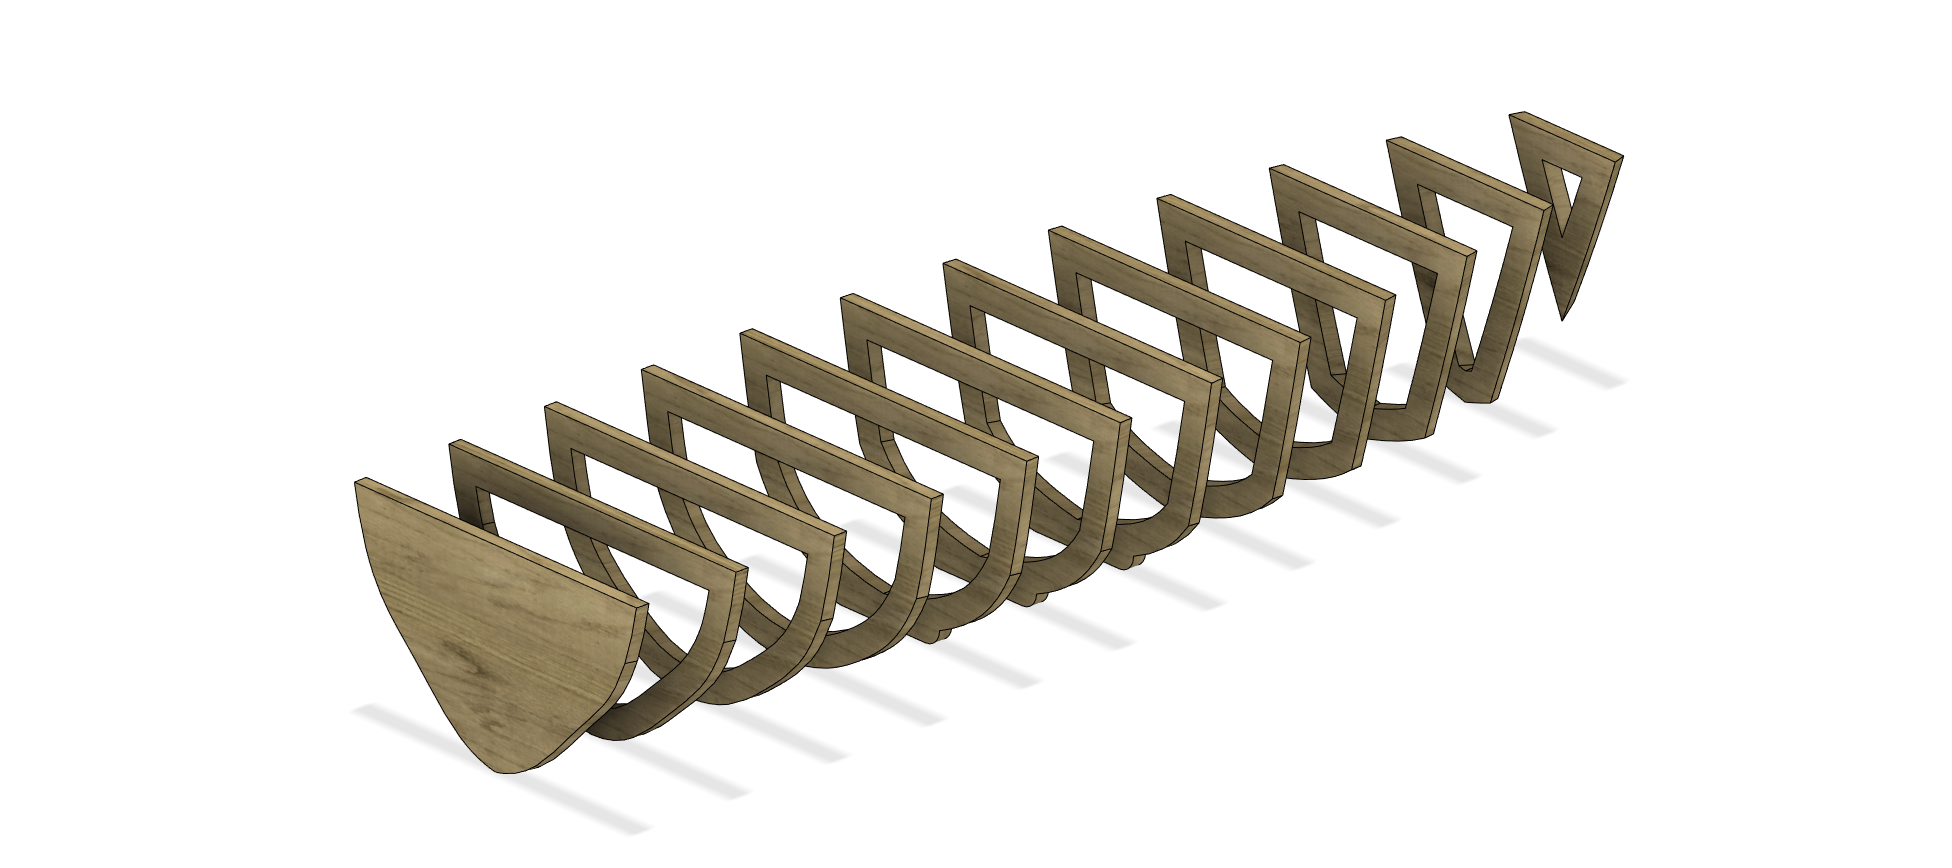
\includegraphics[width=1\linewidth]{assets/rippen_cad.png}
    \caption{Spantenansicht}
    
\end{figure}
Die letzte Spannte, der Achtersteven genannt wir, ist nicht hohl, weil sie sich am Ende des Hohlkörpers befindet und diesen abschliesst.  \\
Der Bug des Bootes läuft spitz zu. Diese Form der Spitze ist in Holz schwierig zu bauen. Es wird daher auf die klassische Konstruktion mit einer Bugspante verzichtet. An ihrer Stelle wird die gesamte Spitze im 3D Druckverfahren aus Kunststoff als ein einziges Werkstück gedruckt. Es wird mit der vordersten Spante verklebt. Der Bugspitz ist nicht in Massivbauweise vorgesehen, sondern als Hohlkörper vorgesehen.
\begin{figure}[H]
    \centering
    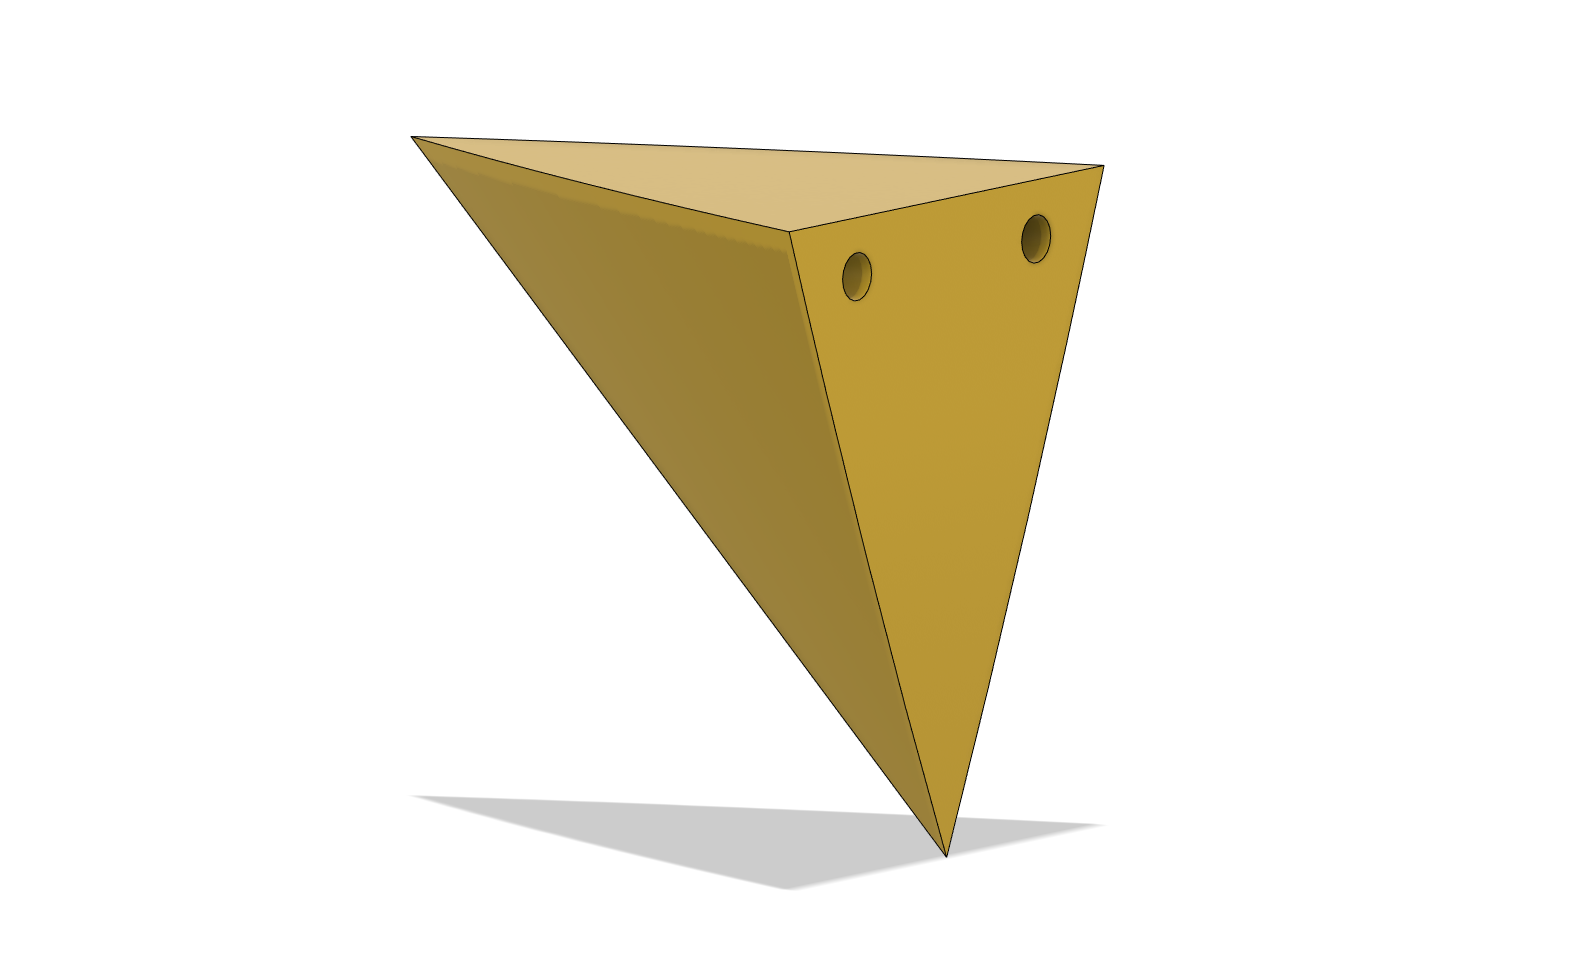
\includegraphics[width=0.8\linewidth]{assets/bug_spitz.png}
 \caption{Bugspitz}
    
\end{figure}
Die meisten Boote und Schiffe verfügen über einen mittschiffs im Boden angebrachten Längsverband, der das Rückgrad des Bootes bildet. An ihm sind die querstabilisierenden Spanten befestigt. Dieser Längsverband bildet zusammen mit einer vertikalen Unterwasserverlängerung den Kiel und mündet am Anfang und Ende in den Steven.  \\
Da für die vorliegende Konstruktion ein Flachdeck vorgesehen ist, der Boden des Schiffskörpers aber gewölbt ist, wird von dieser klassischen Kielkonstruktionsweise abgewichen. Die Längsverbindung der Spanten wird nicht am Boden des Schiffes, sondern direkt unter dem Deck vorgesehen. Sie besteht auch nicht aus einem  einem einzigen mittschiffs angebrachten Längsverband, sondern aus zwei Längsverbänden, die in einem  Abstand von 10 cm von der Mittelachse parallel über die ganze Bootslänge horizontal angebracht werden. Sie bestehen aus zwei Alluminiumröhren mit einem Durchmesser von je 16 mm. Die beiden Röhren werden durch die Spanten geführt, in welchen im oberen Holm je zwei runde Löcher im Abstand von 10 cm gebohrt werden. Am vorderen Ende des Bootes werden die beiden Röhren in zwei dafür vorgesehene Hohlöffnungen des gedruckten Bugspitzes geführt und verklebt.  \\
Diese Konstruktion ist viel einfacher zu bauen als ein klassischer Kielaufbau.  Sie ist bei  bemannten Booten nicht verbreitet, weil die beiden Längsverbindungen direkt unter dem Deck dem Einbau eines Cockpits im Weg stehen würden. Möglich wäre allein das Cockpit auf dem Deck aufzubauen, was sowohl die Stabilität als auch den Komfort stark beeinträchtigen würde. Auch ein  Zugang zu einer Kajüte würde verunmöglicht. 
\begin{figure}[H]
    \centering
    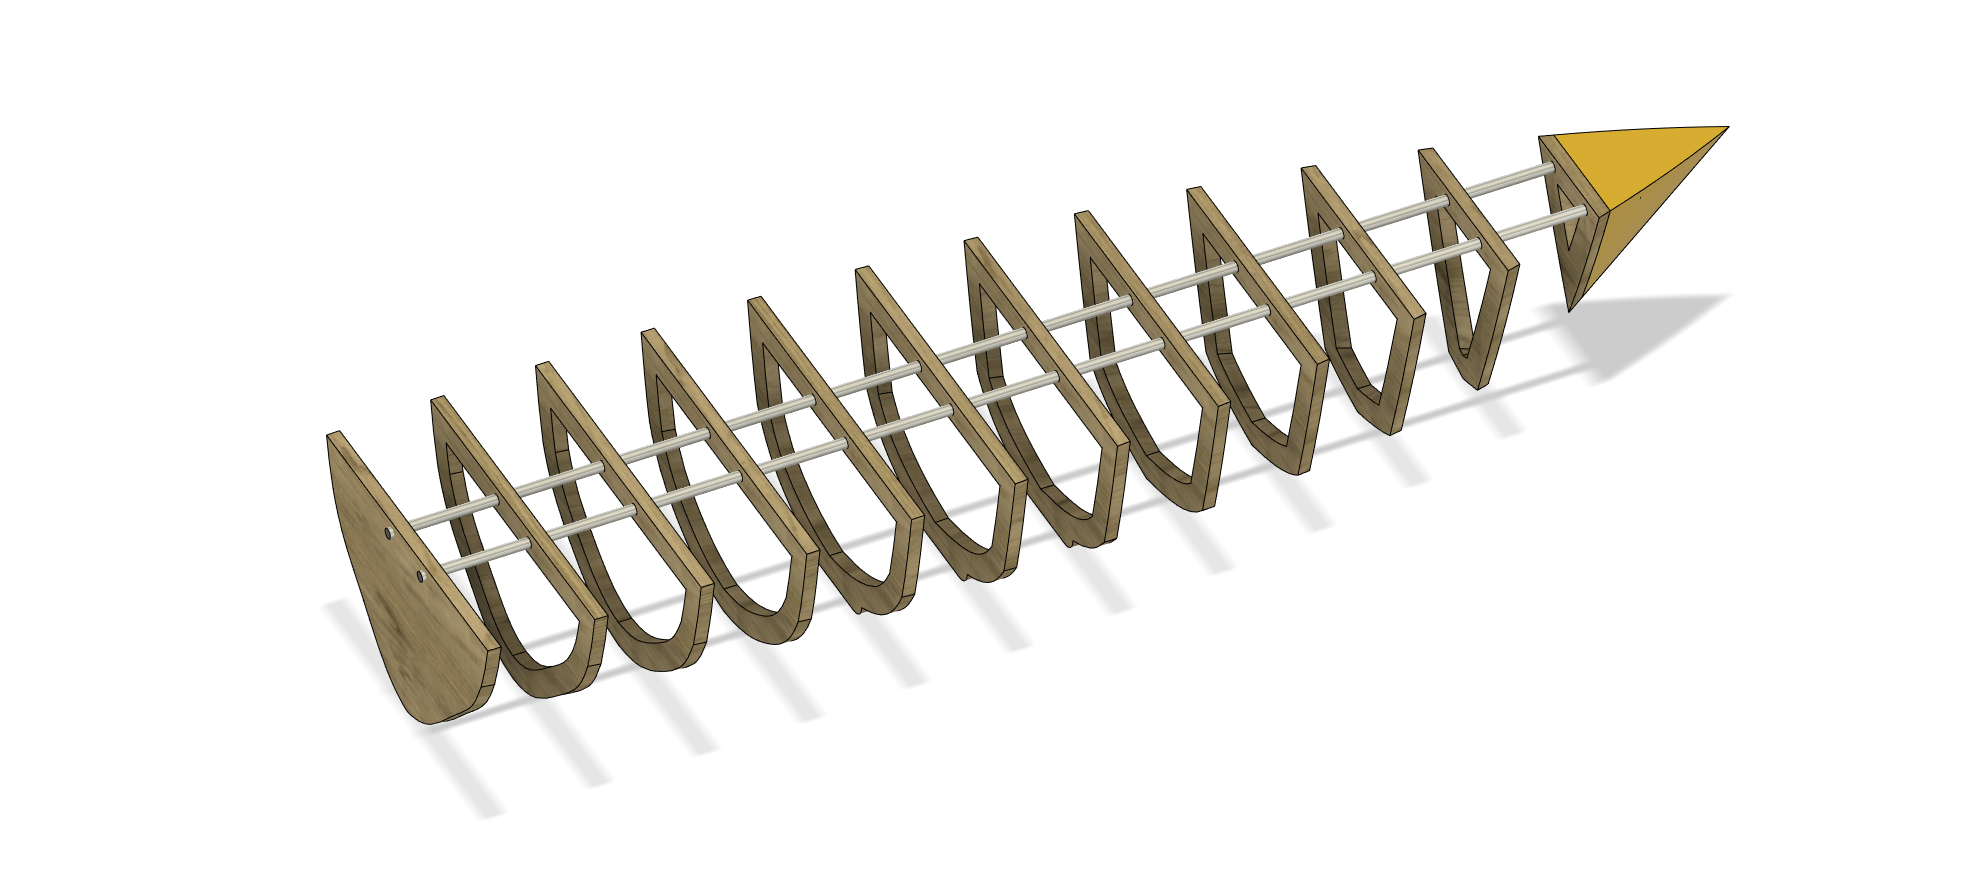
\includegraphics[width=1\linewidth]{assets/full_skellet.png}
    \caption{Abbild der Spanten und des Spitzes in Verbindung}
    
\end{figure}

%\begin{figure}[H]
%  \centering
%  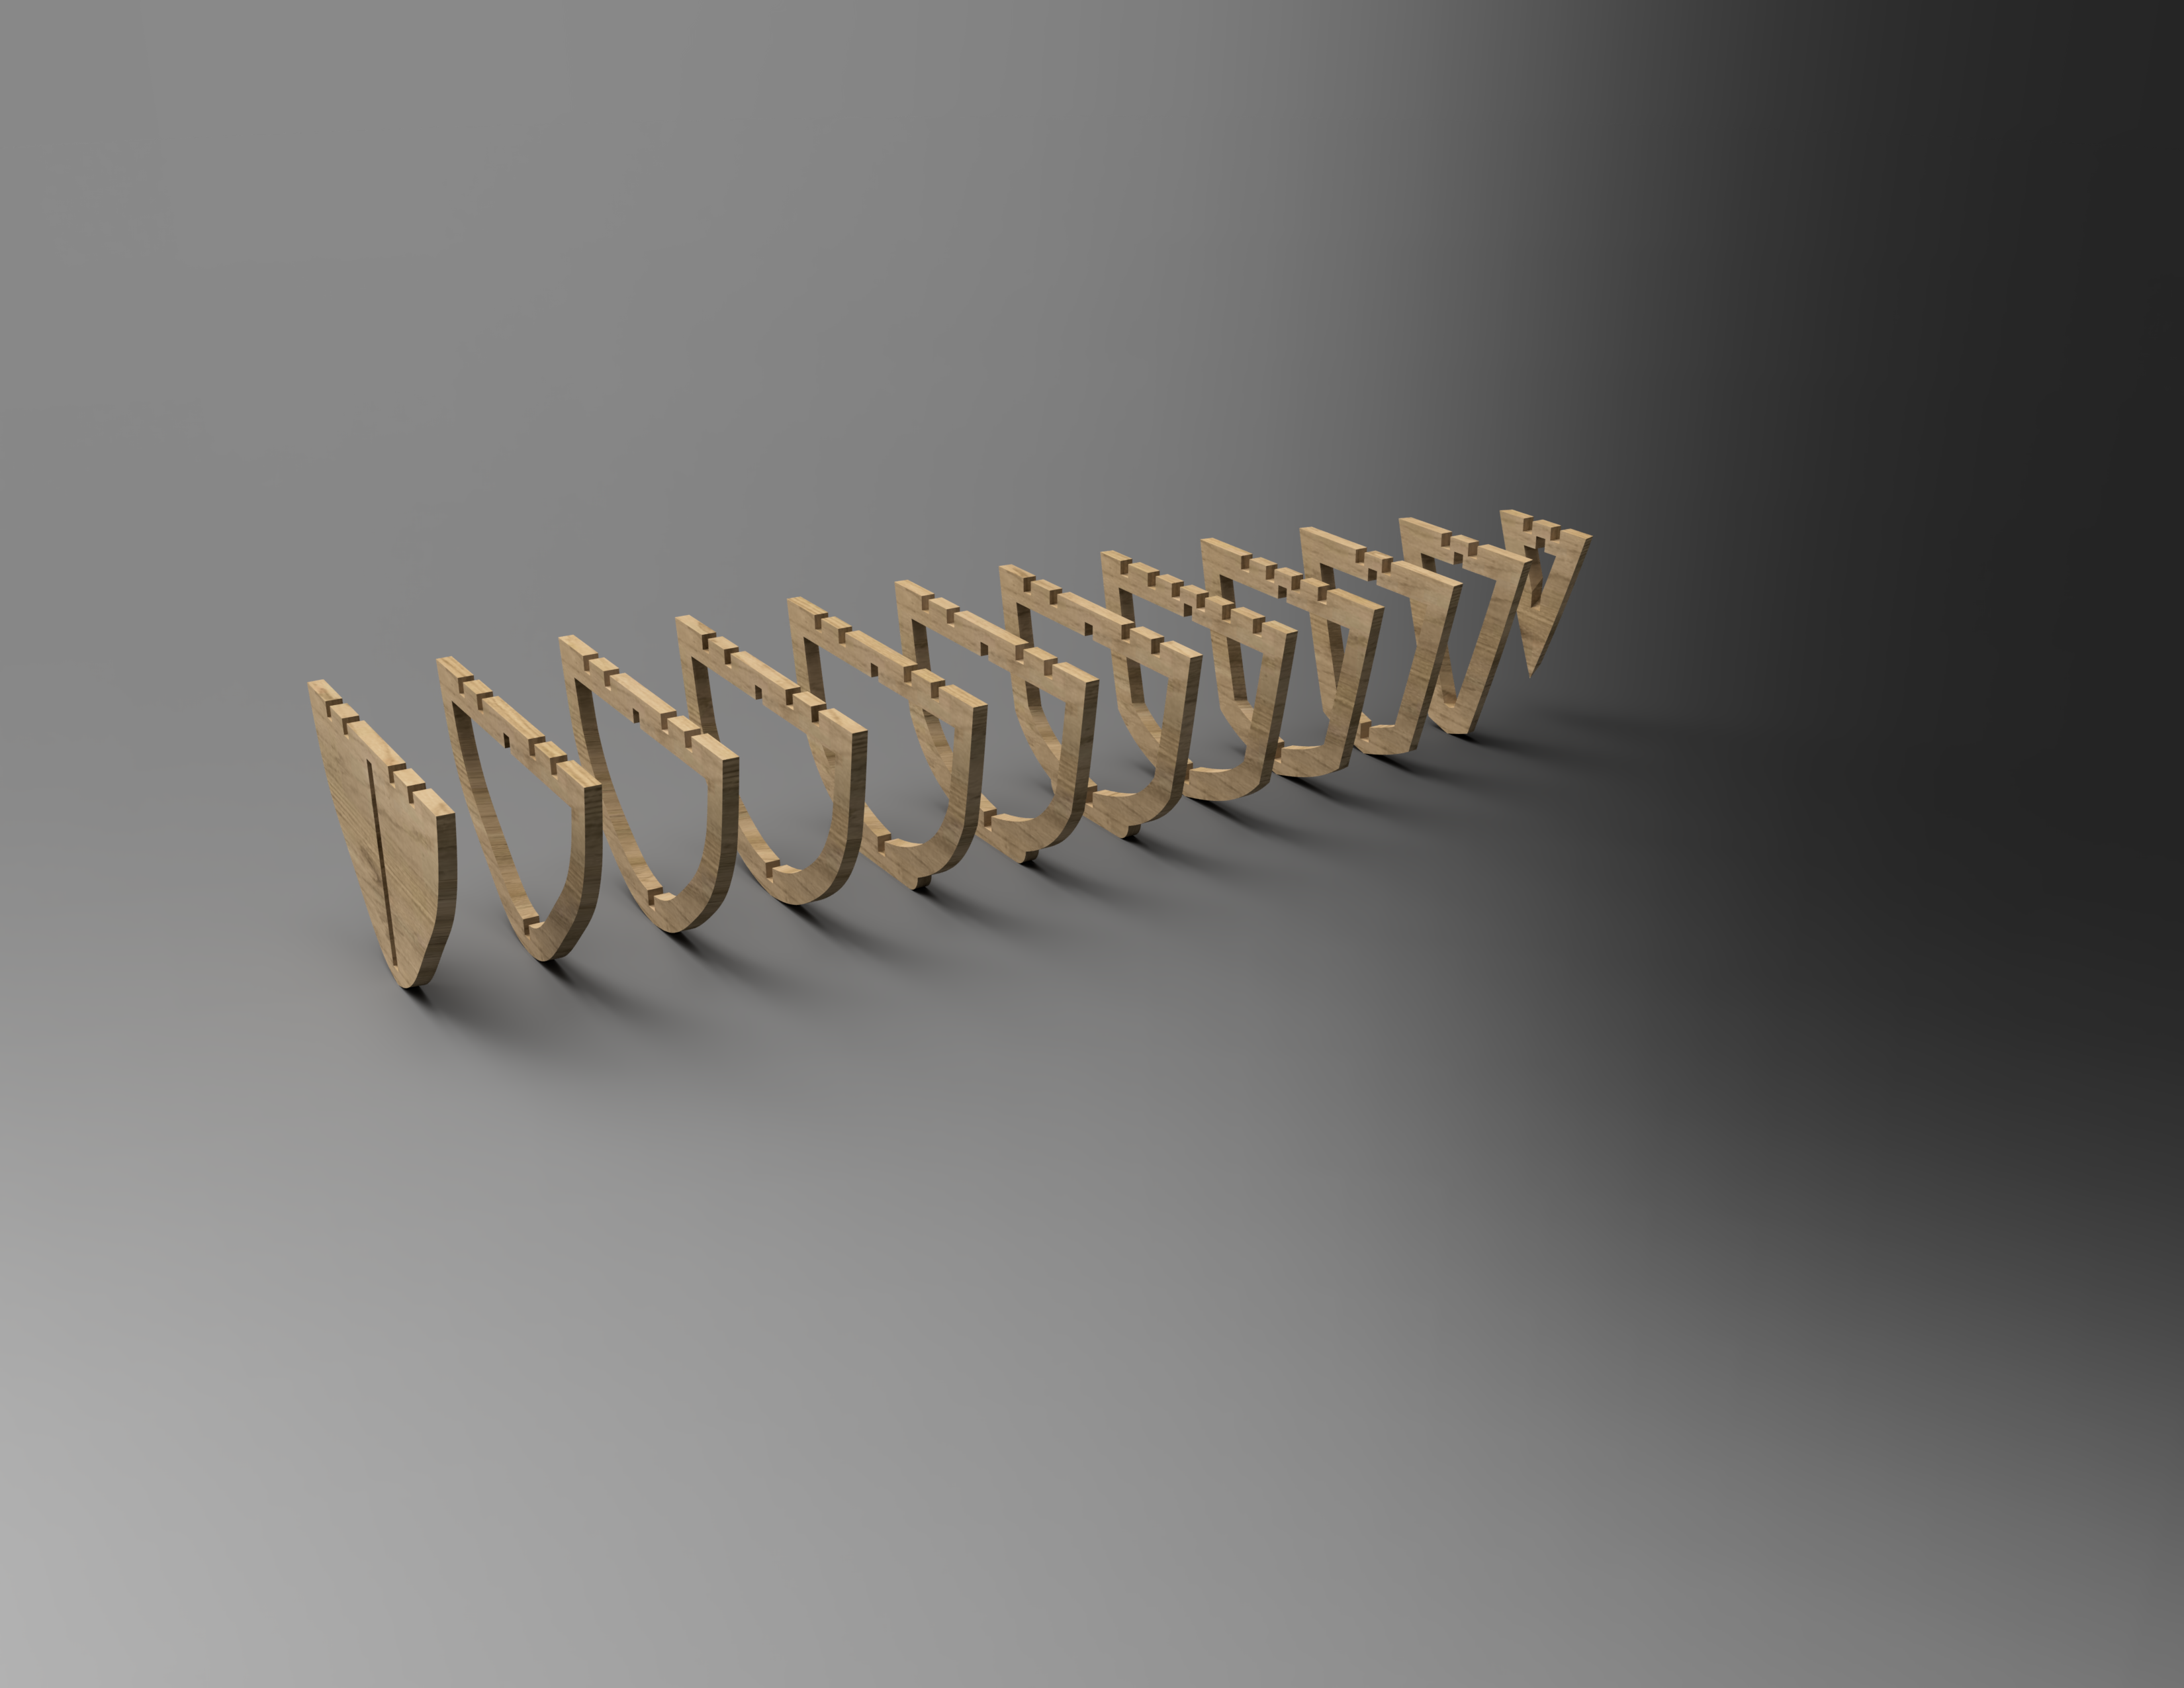
\includegraphics[width=\textwidth]{assets/rippenv1.png}
%  \caption{Render einer ersten Version des Rippenmusters (nicht Final) }
%  \label{fig:rippenv1}
%\end{figure}




\section{Segel und Sailflap}
Beim Design des Segels wird viel von einer bestehenden Arbeit übernommen.[???ARBEITEN ABFFÜHREN???] Diese hat sich mit der Entwicklung eines Segels für den Einsatz auf dem Baltischen Meer beschäftigt.

???

???

\section{Entwicklungsprozess des Kiels}

Bei der  Konstruktion des Bootes wird auf eine klasssische Kielkonstruktion verzichtet, dieses aus Stabilitätsgründen aber zwingend mit einem Balastkiel ausgestatet werden muss, kann dieser nicht wie üblich an der an der Der Kiel hat die Form eines Kurzkiels. Er  wird aus  5  Teilen zusammengesetzt. 


Die meisten Boote und Schiffe verfügen über einen mittschiffs im Boden angebrachten Längsverband, der das Rückgrad des Bootes bildet


Oben wird bei der Beschreibung der Konstruktion des Bootskörpers ausgeführt, dass von der klassischen Bauweise mit einem über die gesamte Länge des Bootes reichenden Kiel abgewichen wird.\\
Der Kiel dient bei Booten aber nicht als Rückgrad der Rumpfkonstruktion, sondern vor allem auch der Stabilisierung des Bootes im Wasser, der Erhöhung der Kursstabilität, sowie, gerade bei Segelbooten sehr wichtig, der Verringerung der seitlichen Abdrift. \\

